\part{No princípio era o meio}

\chapter{O século XX em foco\footnote{``O século \textsc{xx} em foco'' é um capítulo do livro \textit{O século da canção}, publicado em 2004 pela Ateliê Editorial. O livro é um estudo de Luiz Tatit sobre a canção popular produzida no Brasil em todo o século \textsc{xx}. Em ``O século \textsc{xx} em foco'', o autor propõe uma análise do século passado através de grandes canções que marcaram suas épocas.}}

\section{entrada no século}

A prática musical brasileira sempre esteve associada à mobilização
melódica e rítmica de palavras, frases e pequenas narrativas ou cenas
cotidianas. Trata-se de uma espécie de oralidade musical em que o
sentido só se completa quando as formas sonoras se mesclam às formas
linguísticas, inaugurando o chamado gesto cancional. Tudo ocorre como se
as grandes elaborações musicais estivessem constantemente instruindo um
modo de dizer que, em última instância, espera por um conteúdo a ser
dito. Essa espera pode ser muito breve, quando o próprio compositor já
se encarrega também da criação dos versos ou a encomenda a um parceiro
próximo; pode se prolongar por dez anos --- como aconteceu com
``Carinhoso'', a melodia de Pixinguinha que teve seu ciclo de música
instrumental até \textit{se completar} na letra de João de Barro; por
sessenta anos --- como o choro ``Odeon'', de Ernesto Nazareth, composto
em 1908 e que ganhou letra de Vinicius de Moraes em 1968; ou por um
tempo indeterminado, como parece ser o caso de quase todo o repertório
musical brasileiro que ainda não se converteu em canção\ldots

Isso não significa a ausência no país de uma tradição eminentemente
musical, empenhada em desenvolver recursos que independam de qualquer
gênero de oralidade. Acontece que os resultados obtidos nessa esfera de
produção estão longe de representar a principal via da originalidade
brasileira, senão pela qualidade em comparação com a criação musical do
resto do mundo, pelo menos pela quantidade, pouco expressiva se a
confrontarmos com os números exibidos na área da canção. Por isso,
preferimos nos ater ao âmbito que se revelou mais fecundo e,
consequentemente, mais promissor para a entrada do novo milênio.

A canção brasileira, na forma que a conhecemos hoje, surgiu com o século
\textsc{xx} e veio ao encontro do anseio de um vasto setor da população que
sempre se caracterizou por desenvolver práticas ágrafas. Chegou como se
fosse simplesmente uma outra forma de falar dos mesmos assuntos do dia a
dia, com uma única diferença: as coisas ditas poderiam então ser reditas
quase do mesmo jeito e até conservadas para a posteridade. Não é mera
coincidência, portanto, que essa canção tenha se definido como forma de
expressão artística no exato momento em que se tornou praticável o seu
registro técnico. Ela constitui, afinal, a porção da fala que merece ser
gravada.

Entre o lundu, de origem fincada nos batuques e nas danças que os negros
trouxeram da África e desenvolveram no Brasil, e a modinha, cujo caráter
melódico evocava trechos de operetas europeias, um gênero apontando para
os terreiros e o outro para os salões do século \textsc{xix} --- mas ambos já
impregnados de sensualidade híbrida que, muitas vezes, os tornavam
indistintos ---, configura-se a canção do século \textsc{xx}, a esta altura
apontando também para um terceiro elemento que se tornaria vital à sua
identidade: a letra. Não tanto a letra-poema, típica das modinhas, ou a
letra cômico-maliciosa dos lundus, mas a letra do falante nativo, aquela
que já nasce acompanhada pela entoação correspondente. Sem nunca deixar
de lado o lirismo ou mesmo a comicidade que já reinavam no período
oitocentista, a nova letra, que só se consolidou nos anos 1920 com
Sinhô, substituiu o compromisso poético pelo compromisso com a própria
melodia, ou seja, o importante passou a ser a adequação entre o que era
dito e a maneira (entoativa) de dizer, bem mais que o valor intrínseco
da letra como poema escrito ou declamado.

Justamente por não ser nem demasiadamente percussiva nem demasiadamente
\textit{musical}, como o chorinho, por exemplo, que se nutria de requintadas
sutilezas instrumentais, essa nova canção ganhou, como já expusemos, a
concorrência para as primeiras gravações. Dos batuques emanavam um
volume de som incompatível com os parcos recursos de gravação
implantados pelos primeiros grupos de fonógrafos que aportaram no Rio de
Janeiro. De outra parte, os mestres do chorinho e de outros gêneros de
música escrita não viam razão para trocar sua forma precisa de registro
em partitura pelos meios fonomecânicos rudimentares que jamais
expressariam todos os matizes musicais de suas composições. As canções,
ao contrário, por estarem baseadas numa oralidade de natureza instável
 --- também já vimos que a entoação da fala tende a desaparecer assim que a
mensagem do texto é transmitida ---, precisavam da gravação como recurso de
fixação das obras que, até então, quando não se perdiam nas rodas de
brincadeira, passavam a depender exclusivamente da boa memória de seus
praticantes.

Assim, ao convidar cantores de música popular, como Cadete e Baiano,
para testar a nova tecnologia de registro sonoro, o pioneiro Frederico
Figner não sabia que, para solucionar o problema prático de inserção de
um produto no mercado, estava consagrando definitivamente a oralidade
brasileira. Realmente, a partir desse instante, jamais se interrompeu o
fluxo de criação e perpetuação das formas cantáveis da fala, gerando no
Brasil uma das tradições cancionais mais sólidas do planeta.

\section{princípio entoativo}

Um fenômeno recorrente na história da canção brasileira chama a atenção
dos pesquisadores que empreendem seus estudos pelo viés musical. Por
mais que os ambientes sonoros, nos quais surgiram as melhores obras do
repertório nacional, tenham sido marcados pela presença de músicos
competentes, maestros arranjadores ou instrumentistas notáveis, o centro
de criação dessas obras sempre esteve nas mãos de outros artistas,
amplamente reconhecidos como compositores e letristas de sucesso, que em
geral exibiam pouca intimidade com a linguagem musical. Evidente que
quase todos dispunham de boa musicalidade, no sentido de reter melodias
na memória, reproduzir ritmos percussivos, tocar instrumentos de ouvido,
mas isso não significa que conseguissem traduzir intelectualmente o que
eles próprios realizavam. As chamadas divisões de compasso, a concepção
harmônica, a orquestração e, no final das contas, a partitura escrita
sempre ficavam a cargo dos especialistas, que, por sua vez, embora
fossem mestres em estabelecer essas conversões e em corrigir soluções
malformadas, não ousavam assumir o papel desses artistas
\textit{despreparados} na fase da criação. Os músicos conhecedores da
tradição escrita, mas que tiravam o seu sustento de atividades na faixa
popular, sempre devotaram especial respeito aos compositores que sabiam
aliar melodias a letras independentemente de seu nível de formação
musical.

Isso configura um sintoma precioso para calibrar os critérios de
avaliação dessa produção popular. Antes de tudo, o que assegura a
adequação entre melodias e letras e a eficácia de suas inflexões é a
base entoativa. De maneira geral, as melodias de canção mimetizam as
entoações da fala justamente para manter o efeito de que cantar é também
dizer algo, só que de um modo especial. Os compositores baseiam-se na
própria experiência como falantes de uma língua materna para selecionar
os contornos compatíveis com o conteúdo do texto. Tal princípio
entoativo é, ao mesmo tempo, simples e complexo.

É simples porque o foco de sentido de uma curva entoativa concentra-se
sobretudo em sua finalização, ou seja, nas inflexões que antecedem as
pausas parciais ou o silêncio derradeiro. Essas inflexões, denominadas
tonemas, podem ser descendentes, ascendentes ou suspensivas, quando
sustentam a mesma altura. A descendência está cultural e
tradicionalmente associada a conclusões de ideias. A distensão da curva
indica que, em princípio, não há nada a acrescentar. É evidente que, por
contraste, as duas outras formas, ascendente e suspensiva, perfazem a
tensão típica da continuidade: ou temos uma pergunta, explícita ou
implícita, ou temos a informação sub-reptícia de que o discurso deve
prosseguir, ou, ainda, temos o indício de que algo ficou suspenso. Ao
adotar espontaneamente esses tonemas da fala cotidiana, fazendo-os
coincidir --- também espontaneamente --- com os momentos afirmativos,
continuativos e suspensivos da letra, o compositor já responde por uma
compatibilidade natural entre os dois componentes da canção, e já
determina um primeiro grau de cumplicidade com o ouvinte que reconhece,
em geral também sem ter consciência, os recursos típicos de sua língua
materna.

Mas esse princípio entoativo possui igualmente uma dimensão mais
complexa. Além do paralelismo já mencionado entre frases ou versos e
suas respectivas entoações, que permanece de fundo em toda e qualquer
canção, há encaminhamentos melódicos de largo alcance que expandem as
enunciações para ascendências ou descendências distantes, de maneira que
os segmentos parciais passam a ser definidos também pela direção extensa
com a qual estão comprometidos. E, durante o percurso melódico, outros
recursos vão sendo ativados, prestigiando ora a configuração rítmica,
ora a orientação melódica. No primeiro caso, temos a forma concentrada
de composição: a elaboração musical tende para a construção de temas e
de refrões, como marchinhas de carnaval, música axé e toda a sorte de
canções dançantes. No segundo, temos a forma expandida em que os
motivos melódicos tendem a se diluir em favor das trajetórias realçadas
pela evolução mais lenta das notas musicais, como no caso dos boleros e
das canções românticas em geral.

Os cancionistas são os artesãos dessa forma de compor que tem por base
--- entre outras coisas, mas acima de tudo --- as inflexões entoativas
da fala cotidiana. São os herdeiros de Cadete e de Baiano, e ostentam
como habilidade principal a criação de melodias e letras fortemente
compatibilizadas, sem que, para isso, disponham necessariamente de
formação musical ou literária. Embora nada devessem à tradição escrita
da música e da literatura, muitos cancionistas dos primeiros tempos,
como Catulo da Paixão Cearense, Cândido das Neves, Heckel Tavares,
Orestes Barbosa ou mesmo, nos anos 1930, Ary Barroso, sentiam um certo
desgosto por não praticar uma arte já suficientemente reconhecida pelos
povos colonizadores. Isso transparece em melodias grandiosas ou em
versos empolados produzidos por esses artistas, como que tentando dizer
que os grandes conteúdos não podiam ser expressos por um formato tão
singelo como o da canção. Ao mesmo tempo, defendiam a linguagem popular
para o tratamento dos assuntos cotidianos e, assim, acabavam por
produzir uma obra desigual, mas nem por isso menos importante para a
consolidação da prática que se iniciara com o século. Outros, como Noel
Rosa, Ismael Silva, Wilson Batista, Lamartine Babo ou Assis Valente,
jamais manifestaram qualquer indício de frustração com a militância
cancional. Noel, por exemplo, dedicou inúmeras letras ao tema do
\textit{orgulho em ser sambista}, o que constituía um signo de altivez e de
total segurança com relação ao poder de sedução da nova linguagem.

\section{os cancionistas}

Os cancionistas firmaram-se de vez na década de 1930. A vasta produção
desse período consagrou a entoação da linguagem oral como centro
propulsor de todas as soluções melódicas que resultaram nos gêneros e
estilos até hoje praticados. Bem mais poderosa que os tradicionais
recursos enunciativos de ancoragem na primeira pessoa, no \textit{eu lírico},
a entoação atrela a letra ao próprio corpo físico do intérprete por
intermédio da voz. Ela acusa a presença de um \textit{eu} pleno, sensível e
cognitivo, conduzindo o conteúdo dos versos, e inflete seus sentimentos
como se pudesse traduzi-los em matéria sonora. De posse dessa força
entoativa, e valendo-se do poder de difusão das ondas radiofônicas, os
cancionistas se esmeraram em fazer dos intérpretes personagens definidos
pela própria entoação. Ouvia-se, então, a voz do malandro, a voz do
romântico, a voz do traído, a voz do embevecido, a voz do folião, todas
revelando a intimidade, as conquistas ou o modo de ser do enunciador.

A partir desse princípio geral, foram se estabilizando os tipos de
compatibilidade entre melodia e letra já mencionados anteriormente.
Melodias que tendiam à contração, seja pelo andamento acelerado, seja
pelas frequentes reiterações temáticas, serviam às letras de celebração
das uniões, das aquisições, enfim, dos estados de plenitude. ``Chiquita
bacana'', de João de Barro e Alberto Ribeiro, ``Camisa listrada'', de Assis
Valente, e ``Samba da minha terra'', de Dorival Caymmi, são exemplos de
canções, concentradas no refrão, cujas entoações cíclicas indicam
identidade entre elementos melódicos, do mesmo modo que, na letra, os
sujeitos aparecem em perfeita conjunção com os respectivos objetos de
desejo. Melodias que tendiam à expansão lenta de seu percurso no campo
de tessitura, apontando para regiões sonoras mais distantes dos refrões,
pediam letras que de alguma forma configuravam situações disjuntivas, de
abandono, mas com horizontes de conjunção projetados tanto sobre o
passado --- saudades, lembranças etc. --- como sobre o futuro --- esperanças,
projetos etc. ``O ébrio'', de Vicente Celestino, ``Pra machucar meu
coração'', de Ari Barroso, e ``Lábios que beijei'', de \textsc{j}.\,Cascata e Leonel
Azevedo, contêm esse tipo de melodia que se desdobra vagarosamente em
rotas evolutivas, descrevendo musicalmente as tensões disjuntivas, da
perda ou da falta do objeto, responsáveis pelas emoções do sujeito no
plano da letra. Outras melodias ainda mantinham relativamente
desativados seus recursos de concentração temática ou de expansão
passional dos contornos para apresentar, \textit{hic et nunc}, a voz do
enunciador dizendo algo considerado oportuno. Com inflexões similares às
da linguagem oral cotidiana, essas melodias geralmente conduziam
\textit{letras de situação}, aquelas que simulam que alguém está falando
diretamente com alguém em tom de recado, desafio, saudação, ironia,
lamentação, revelação etc. ``Palpite infeliz'' ou ``Até amanhã'', de Noel
Rosa, ``Minha palhoça'', de \textsc{j}.\,Cascata, e ``Acertei no milhar'', de Wilson
Batista e Geraldo Pereira, são canções típicas desse estilo cancional, o
mais próximo da raiz entoativa.

Percebendo a força enunciativa da canção popular no final da década de
1930, o Estado Novo de Getúlio Vargas chegou a encomendar aos
compositores temas mais \textit{edificantes} e, sobretudo, posturas mais
disciplinadas e pedagógicas para os personagens gerados na instância do
\textit{eu}. Seria útil ao regime ditatorial recém-instalado que os
influentes enunciadores da canção trocassem o tema da orgia, do amor e
do samba pelo do trabalho e da vida regrada. Quanto ao samba, este já
estava de tal forma disseminado na vida do povo brasileiro que tentar
substituí-lo por gêneros de música culta seria um ato condenado ao
fracasso.

Embora contasse com a adesão --- provavelmente interessada --- de alguns
poucos compositores populares, a empresa não pôde prosperar já que, em
última instância, os propósitos governamentais abalariam a própria
compatibilidade entre melodia e letra. Não é difícil forjar um tema e um
comprometimento enunciativo na letra. O embaraço está em sustentar uma
simulação melódica. A entoação, como já vimos, descreve sem
intermediação o perfil do enunciador, com todas as crenças, convicções
--- inscritas, por exemplo, nas descendências asseverativas ---, dúvidas,
ironias, hesitações, enfim, com todas as modalidades afetivas e
cognitivas que definem a personalidade do sujeito. Essa espécie de
\textit{sinceridade} melódica não pode ser dissimulada por muito tempo, sob
pena de esmorecer o próprio gesto composicional. Foi assim que as
canções de sucesso continuaram exaltando os valores pouco ortodoxos do
povo boêmio, expressando-se pelas três principais vias --- temática,
passional e enunciativa --- examinadas anteriormente e fazendo das
décadas de 1940 e 1950 o período de sua grande difusão radiofônica por
todo o Brasil.

\section{a era moderna}

A partir de 1955, disputando o mercado com o bolero e o tango que aqui
aportavam, os produtores e intérpretes passaram a encomendar aos
compositores cada vez mais sambas-canções --- a versão brasileira dos gêneros
hispano-americanos ---, no ensejo de conquistar o imenso público que se
formava em torno desse segmento passional. Se por um lado o projeto teve
êxito, por outro gerou significativa perda de audiência no âmbito dos
jovens, principalmente entre os estudantes. Quando não vem compensada
pelos recursos da tematização e da enunciação oral, a dicção romântica
corre o risco de adquirir excessos sentimentais que beiram o melodrama.
Isso costuma afastar o público --- em geral, mais abastado --- que se
envolve de forma mais objetiva e técnica com o mundo musical. Tal
perspectiva mais a notória influência do cool jazz absorvida por
importantes nomes que começavam a ingressar, desde o início da década,
no cenário musical brasileiro --- Dick Farney, Lúcio Alves, Johnny Alf, Tom
Jobim --- deram condições para a primeira tomada de posição estética
ocorrida no interior da música popular brasileira. Por volta de 1958, em
plena euforia do período \textsc{jk}, alguns violonistas, pianistas e cantores
muito jovens, a maioria proveniente da classe média carioca e dos
circuitos universitários, celebravam o nascimento da bossa nova. Foi o
primeiro movimento com núcleo na música popular que se espraiou por
vários setores da sociedade brasileira, do estético ao político,
fundando um novo modo de ser.

Importa-nos comentar as principais dicções que deram personalidade
estética ao movimento: a de Tom Jobim e a de João Gilberto. Ao compor
``Tereza da praia'', de 1954, com o sambista Billy Blanco, Tom Jobim já
anunciava a prática, que seria uma constante no período seguinte, de
substituir a oratória passional pela linguagem coloquial. Ainda se
atendo às generosas inflexões melódicas em voga, os autores não deixavam
de reativar as entoações em sua expressão mais adequada ao diálogo
natural e direto. Além disso, o compositor carioca enveredava pelas
dissonâncias provenientes do jazz com a função precípua de condensar
efeitos emocionais, antes inscritos na vasta expansão dos contornos e no
encadeamento harmônico de base das canções. O emprego dos novos acordes
sugeria novas direções --- e, portanto, novos sentidos --- melódicas que
jamais poderiam constar das sequências de tríades perfeitas até então
adotadas. Aos poucos, Jobim foi também eliminando do acompanhamento toda
a sorte de notas supérfluas que não contribuíssem diretamente para a
caracterização da função harmônica.

A única maneira de apreciar essa nova canção, com os parâmetros da
época, era por aproximação às soluções musicais norte-americanas que, no
pós-guerra, tornaram-se modelo de qualidade em todas as culturas que as
consumiam pelas rádios, pelos filmes de Hollywood ou pelos discos
importados. Mas ficou claro com o tempo que o verdadeiro gesto de Jobim
apontava para outra direção. Toda a influência do jazz foi utilizada na
reabilitação das dicções, enunciativa e temática, que vinham sendo
sistematicamente neutralizadas pelo sucesso popular da dimensão
passional.

Essa intervenção na música brasileira fica ainda mais definida com a
participação radical do violonista e intérprete baiano João Gilberto.
Esse cancionista adota a nova inteligência harmônica que impregnava
nossa música dos anos 1950, mas a incorpora em acordes compactos que, no
violão, favorecem a condução percussiva. Com isso, reencontra a batida
do samba sem precisar enfatizar seus tempos fortes que, a esta altura,
já eram considerados suficientemente assimilados pela cultura musical
brasileira. Mencionamos também o \textit{toque de tamborim} que o cantor
incorpora em sua batida, e mesmo o ajuste da voz, calibrada no volume da
fala cotidiana, que se adapta à articulação precisa das unidades
temáticas, deixando-as flutuar sobre a batida de fundo dos acordes sem
muita dependência rítmica. Falta comentarmos sua escolha das letras.
João Gilberto dispensa todo e qualquer excesso que possa resvalar no
dramático, e passa a escolher canções que falem do próprio gênero --- ``Samba da minha terra'', de Dorival Caymmi, ``Samba de uma nota só'', de Tom Jobim e Newton Mendonça --- , que tratem de conteúdos leves, quase
infantis --- ``Lobo bobo'', de Carlos Lyra, ``O pato'', de Jayme Silva e Neuza Teixeira, e ``Bolinha de papel'', de Geraldo Pereira --- ou de
amores que fluem ou tendem a fluir sem sofrimento passional --- ``Amor em
paz'', de Tom Jobim e Vinicius de Moraes, e ``Corcovado'', de Tom Jobim.

Nesse sentido, a bossa nova de Tom Jobim e João Gilberto aprumou a
canção brasileira expondo o que lhe era essencial. Essa triagem dos
traços fundamentais deu origem ao que hoje podemos chamar de
protocanção, uma espécie de grau zero que serve para neutralizar
possíveis excessos passionais, temáticos ou enunciativos. Isso não
significa que os excessos não sejam bem-vindos, ou que não garantam a
saúde da linguagem cancional. São eles que transpõem os limites
consagrados pelo uso e pelo senso comum. São eles que ultrapassam as
barreiras dos gêneros e dos estilos, pondo em risco a própria existência
da linguagem como campo específico de comunicação. Sem os excessos a
canção perderia sua força de experimentação, tanto estética como
comercial. Mas a bossa nova, cuja marca é justamente a da decantação,
não os suporta. Toda vez que um cancionista --- roqueiro, pagodeiro,
tecno, sertanejo, vanguardista etc. --- sente a necessidade de fazer um
recuo estratégico para recuperar as linhas de força essenciais de sua
produção, o principal horizonte que tem à disposição é a bossa nova. Ela
oferece elementos para decantar o gesto fundamental dos artistas dos
sedimentos passionais, maneiristas, ou mesmo viciosos, que muitas vezes
imobilizam o trabalho musical. Não se trata de compor como Tom Jobim ou
de cantar como João Gilberto, mas sim de descobrir os fatores básicos e
determinantes do próprio estilo. Quase todos os grandes nomes do final
do século \textsc{xx} --- como Caetano Veloso, Rita Lee, Cazuza, Gal Costa,
Titãs, Gilberto Gil, Tim Maia etc. --- já tiveram seu período
bossa nova. A série de gravações \textit{acústicas} promovida pela \textsc{mtv}
brasileira a partir dos anos 1990 não deixava de ser uma proposta
bossa nova para revitalizar a carreira dos artistas.

Com o encerramento da era de Juscelino e o crescimento dos conflitos
políticos, acirrados pela evolução das forças de esquerda no país, a
canção brasileira entrou nos anos 1960 manifestando progressiva
tendência ao engajamento ideológico. Os herdeiros da bossa nova, aliados
aos novos expoentes do teatro e do cinema da época, procuraram dar mais
consequência a seus trabalhos a partir de um contato direto com o samba
e com os sambistas de raiz. Sob a direção de Augusto Boal, Nara Leão
apresentou, em 1964, com Zé Keti e João do Vale, o show \textit{Opinião}. Pouco
depois, sob o comando de Elis Regina, o programa \textit{O Fino da Bossa},
promovido pela \textsc{tv} Record de São Paulo, tornou-se a residência
\textit{oficial} da música brasileira, que, uma vez por ano, fazia dos
célebres festivais da música popular brasileira o seu campo de batalha.
Foi quando surgiu a expressão \textsc{mmpb}, Moderna Música Popular Brasileira,
depois reduzida para \textsc{mpb}, cuja correspondência com siglas de partidos
políticos não era de todo casual.

Especialmente imbuídos da dicção de Tom Jobim e de João Gilberto, os
compositores Caetano Veloso e Gilberto Gil começaram a depreender da
música popular uma conduta excessivamente unidirecional, do ponto de
vista estilístico e ideológico, que chegava restringir e até certo ponto
estereotipar a criação brasileira. Para tratar de conteúdos nacionais,
em que predominava a utopia de uma nova sociedade em um novo tempo,
boa parte dos compositores havia apostado na recriação de uma música
fundada em motivos folclóricos, em contextos rurais e em instrumental
típico de certas regiões, atrelando a desejada revolução político-social
à consciência da própria identidade e à autenticidade dos valores
defendidos. Todos os autores da \textsc{mpb} participavam, com maior ou menor
convicção, desse ideário cujas diretrizes, embora não explicitadas, eram
acatadas como senha de um comportamento de esquerda.

Tal conduta unidirecional, que se convertera em verdadeira bula para a
produção de canções competitivas no âmbito dos festivais, não era em si
um problema para a sonoridade brasileira. Afinal, surgiram compositores
de grande fôlego criativo, como Edu Lobo, Milton Nascimento etc., bem como
obras antológicas, calcados nesse espírito da época. O que incomodava os
ouvidos dos futuros tropicalistas era a progressiva atitude de exclusão
adotada pela \textsc{mpb}. Não havia lugar para o rock internacional, que vivia
um apogeu admirável com os fenômenos Beatles, Rolling Stones, Janis
Joplin e Jimi Hendrix, entre outros, e muito menos para a singela
réplica nacional dessa música lançada pela despretensiosa Jovem Guarda.
Também não havia espaço para a canção passional, considerada \textit{cafona}, ou \textit{brega}, como passou a ser chamada mais tarde, e tão \textit{alienada}
quanto a da Jovem Guarda, para o samba coloquial --- aquele que, em última
instância, transmitia a fala popular do malandro --- e, a esta altura, nem
mesmo para a bossa nova, com suas letras dessemantizadas.

Se essa atitude exclusivista não pode ser atribuída indiscriminadamente
a todos os representantes da \textsc{mpb} sediados à época na \textsc{tv} Record de São
Paulo --- Chico Buarque, por exemplo, jamais agiu nessa direção ---,
certamente ela caracterizou a intervenção da linha de frente do
movimento como um todo, ocupada pela canção de protesto, e se instalou
simbolicamente em pequenos gestos de artistas que mantinham
incontestável liderança musical no meio; Geraldo Vandré, porta-voz-mor
da música destinada à \textit{conscientização das massas}, talvez tenha sido
o caso mais típico de manifestação dessa atitude.

É evidente que as tais condutas exclusivistas não constituíam estratégia
previamente equacionada por seus líderes, como se dá constantemente na
área política ou publicitária, com o propósito deliberado de vencer a
concorrência. Tudo indica que os representantes do segmento \textit{protesto}
acreditavam sinceramente que a ocupação dos disputados espaços no mundo
da canção por uma ala revolucionária, no sentido político do termo, 
seria algo de grande importância para o país. Como sempre, porém, nos
meios escolhidos para se atingir o objetivo final de transformação,
ficam consignadas as intenções inconscientemente mascaradas e que, com o
tempo, vão se revelando até mesmo a seus próprios portadores.

Um dos méritos dos tropicalistas foi o de intuir, no calor da hora, a
existência do projeto de exclusão e aplicar-lhe \textit{incontinenti} o antídoto
adequado. Caetano e Gil apostaram então todas as suas fichas na
diversidade, no reconhecimento de todos os estilos que compuseram a
sonoridade brasileira, sem qualquer restrição de ordem nacionalista,
política ou estética. Mais do que isso, os compositores incorporaram o
mercado e suas leis tipicamente
capitalistas como um aliado na luta por essa pluralidade musical. Entre
as primeiras medidas tropicalistas de impacto estavam, portanto, as
visitas de seus líderes aos programas do Roberto Carlos e do Chacrinha.

Do ponto de vista musical, as composições também deixavam transparecer
os sinais da fusão intensamente promovida. Os acordes dissonantes
difundidos pela bossa nova, e tão presentes no nascedouro das carreiras
de todos os herdeiros de João Gilberto, cederam lugar às tríades
perfeitas pré-bossa nova, não por uma volta ao passado, mas porque
caracterizavam o limitado universo musical da Jovem Guarda, bem como o
do rock internacional. Canções como ``Baby'' ou ``Objeto não
identificado'', de Caetano Veloso, lançadas no auge do movimento,
ilustram bem a nova adoção tropicalista. Nas letras, reinavam as
justaposições quebrando a hierarquia sintática das frases ao lado de
temas \textit{improváveis} na tradição cancional brasileira: atitudes
existenciais, modernidade científica e mercadológica, e toda a sorte de
simbologia. O que, por outro lado, impedia uma aproximação pura e
simples entre tropicalismo e Jovem Guarda.

A reinterpretação de canções consagradas do repertório brasileiro, por
sua vez, passou a ter sabor de manifesto, de anexação de setores
esquecidos, marginais ou estigmatizados para o centro do movimento
tropicalista. Essa prática foi sendo sistematicamente reiterada,
sobretudo, por Caetano Veloso, desde sua versão de ``Coração materno'', de Vicente Celestino, incluída no \textsc{lp} Tropicália, até o sucesso retumbante
de ``Sozinho'', de Peninha, nos anos 1990, ambas recuperadas de área
excluída pela elite cultural. E nesses mais de trinta anos que separam a
primeira da segunda gravação, Caetano propôs versão para ``Carolina'', de Chico Buarque --- nesse caso, especificamente, criando-lhe arestas
interpretativas que abalavam a perfeição consensual da gravação original
---, para ``Charles, Anjo 45'', de Jorge Ben Jor, ``Chuvas de verão'', de Fernando Lobo, ``Asa branca'', de Luiz Gonzaga e Humberto Teixeira, ``Tu
me acostumbraste'', de  \textsc{f}.\,Dominguez, ``Na asa do vento'', de \textsc{l}.\,Vieira e João
do Vale, ``Vampiro'', de Jorge Mautner, ``Amanhã'', de Guilherme Arantes,
``Fera ferida'', de Erasmo Carlos e Roberto Carlos, e para canções dos
Beatles, de Michael Jackson, de Bob Dylan e para numerosas outras
composições, sempre nesse espírito de expansão do território
tropicalista.

\section{expansão dos gestos bossa nova e tropicalista}

A bossa nova foi um movimento musical que teve seu apogeu no final dos
anos 1950 e início dos 1960, e foi perdendo o ímpeto estético com a
partida de seus maiores expoentes, Tom Jobim e João Gilberto, para os
Estados Unidos. O período heroico do tropicalismo, por sua vez,
transcorreu nos últimos anos da década de 1960, e foi se desfazendo como
intervenção social também com a partida --- o exílio, neste caso --- para a
Inglaterra de alguns de seus principais promotores, Caetano Veloso e
Gilberto Gil, isso sem contar o \textit{enterro} simbólico do movimento
praticado por seus próprios representantes ao cabo de mais ou menos dois
anos de sua implantação. Se o período explosivo de ambos os movimentos
foi relativamente breve, o poder de influência de suas principais
características sobre toda a produção brasileira posterior parece
perene.

De fato, o gesto de recolhimento e depuração da bossa nova e o gesto de
expansão e assimilação do tropicalismo tornaram-se seiva que realimenta
a linguagem da canção popular toda vez que esta claudica por excesso ou
por espírito de exclusão.

Há excesso quando a canção \textit{diz mas não convence}, em geral por
ignorar o princípio entoativo. O gênero se sobrepõe à particularidade da
composição de tal modo que já nos acordes introdutórios ou na levada
instrumental temos todos os elementos --- de melodia e de letra --- que
deverão comparecer ao longo da canção, como se esta tivesse de obedecer
a uma conduta preestabelecida. Na faixa passional, já mencionamos
exemplos históricos significativos: boa parte dos sambas-canções do
decênio de 1950 e do canto sertanejo dos anos 1990. Na série temática, a
hegemonia do rock na década de 1980, ou, posteriormente, da música axé,
trouxe casos inequívocos de exacerbação estilística. O mesmo poderia
suceder com o rap --- expressão radical da forma enunciativa de compor
--- se, por ventura, se tornasse a bola da vez na mídia televisiva e
radiofônica.

O repertório excessivo passa a não mais convencer porque as soluções
melódicas surgem mais comprometidas com o gênero do que com a letra. São
concebidas para \textit{fazer sentimento} no caso passional, ou para fazer
dançar no caso temático, sem traduzir uma forma singular de dizer o
conteúdo linguístico. Desse modo, as canções deixam de ser especiais e
se contentam com uma audição em bloco. Não havendo nuanças entoativas, a
atenção se dispersa e se embala no que poderíamos chamar de \textit{efeito
muzak}. Só uma atitude bossa nova pode recuperar a raiz oral perdida nos
meandros do gênero.

Por isso, a bossa nova está impregnada na atividade de cada compositor
ou intérprete popular, e se manifesta geralmente em seus momentos de
revisão crítica do próprio trabalho. Está em cada novo disco de João
Gilberto, não por ser a figura maior da fase heroica do movimento, mas
por revigorar, apenas com voz e violão, cada sílaba, cada palavra e cada
entoação das composições que incorpora ao repertório. Está em propostas
arrojadas de reinterpretação que remanejam canções de uma determinada
faixa de audição para outra mais refinada: Caetano Veloso interpretando
``Asa branca'', ``Sonhos'' ou ``Sozinho''; Maria Bethânia interpretando
``É o amor'', Jorge Ben Jor interpretando ``Pois é'' etc. Está, até
mesmo, em grandes iniciativas empresariais, como os já mencionados
projetos acústicos e as reedições dos célebres festivais da música
popular brasileira, que têm a função essencial de estabelecer, vez por
outra, uma triagem nas produções do mercado musical.

Há um espírito de exclusão no mundo da música popular quando algumas
modalidades cancionais --- de ordem passional, temática ou enunciativa
--- são segregadas e, em certa medida, estigmatizadas pelas formas
hegemônicas no mercado ou pelas formas de maior prestígio no âmbito da
elite popular. Esse processo de exclusão atinge igualmente os gêneros de
sucesso, tradicionais ou da moda, e as chamadas produções alternativas.
No caso destas, é fácil entender. O mercado chega a um tipo de música
correspondente a um padrão de vendas, e sonega espaço e oportunidades
para o ingresso de outros modos de \textit{fazer música}. Só quando o modelo
exaure surgem as formas substitutivas que devem reproduzir mais uma vez
o êxito já conquistado. Essa atividade bloqueia uma gama expressiva de
conteúdos sociais e psíquicos que, a partir de um certo ponto, começam a
despontar aqui e ali, em pequenos eventos, como expressão de uma espécie
de guerrilha musical. Nessa linha, assistimos às intervenções
experimentais de músicos paulistas no início dos anos 1980, à emergência
do rock nacional durante a mesma década, ao movimento mangue beat nos
anos 1990, juntamente com as explosões criativas de Carlinhos Brown,
Arnaldo Antunes, Lenine e Chico César, entre outros.

Mas há também a estigmatização dos gêneros de sucesso pelo fato de
fazerem\ldots sucesso. Tom Jobim já havia denunciado essa prática na fase
derradeira de sua vida. Como a reprodução em série exige uma dose
considerável de padronização, as canções preparadas para o consumo de
massa chegam ao mercado com características bastante previsíveis, o que
desagrada profundamente à elite popular. Ofuscados pelo brilho das
cifras astronômicas, dos megaeventos e da cumplicidade do povo
desprevenido, os representantes dessa elite não conseguem enxergar
aspectos positivos nesses empreendimentos vultosos que tomam de assalto
os principais meios de comunicação.

Ora, o gesto tropicalista não admite esse tipo de exclusão. Assim como
parte da população precisa dos conteúdos veiculados pelas produções
diferenciadas e de menor alcance em termos de consumo, outra parte
(quantitativamente bem maior) necessita visceralmente dos \textit{excessos}
eufóricos ou românticos divulgados no grande mercado musical. E não se
trata apenas de fabricação de gosto. Dos incontáveis empreendimentos
associados a grupos e artistas, somente alguns vingam por encontrar
respaldo no anseio popular. Segundo o tropicalismo, precisamos de todas
as dicções --- comerciais ou não comerciais --- para que a linguagem
funcione em sua plenitude. Caetano Veloso e Gilberto Gil, representantes
incontestáveis da canção \textit{de qualidade}, jamais deixaram de flertar
com a música comercial e, de quando em quando, promovem um rico
intercâmbio entre as diferentes faixas de consumo.

Em suma, tropicalismo e bossa nova tornaram-se a régua e o compasso da
canção brasileira. Por isso, são invocados toda vez que se pede uma
avaliação do século cancional do país. É como se o tropicalismo
afirmasse: precisamos de todos os modos de dizer; e a bossa nova
completasse: e precisamos dizer convincentemente. 

Em época de exclusão, prevalece o gesto tropicalista no sentido de retomar a pluralidade. Em
época de excesso de maneirismos estilísticos e de abandono do princípio
entoativo, o gesto bossa nova refaz a triagem e decanta o canto
pertinente. Ambos os gestos atuam na própria mente dos compositores e
cantores impelindo-os, ao mesmo tempo, para a diversidade e para o apuro
técnico e estético. É provável que ainda sobrevivam no decorrer do
século \textsc{xxi}, como componentes críticos inerentes ao próprio ofício de
composição, arranjo e interpretação de música popular, e como
responsáveis pelo eterno trânsito do cancionista entre o gosto de
depuração e o desejo de assimilação.

É evidente que os próprios compositores e músicos de modo geral
jamais tiveram consciência dessa matriz entoativa subjacente às canções.
Seu uso era totalmente espontâneo e, em larga medida, camuflado pelos
recursos musicais de fixação das obras. Trata-se, portanto, de uma
constatação retrospectiva proveniente de um enfoque analítico.

Como essas ocorrências são cíclicas, vez por outra revivemos
situação semelhante, ainda que inserida em diferente contexto histórico,
mercadológico e estético. A hegemonia do samba-canção dos anos 1950 pode
ser associada, guardadas as devidas proporções de consumo, ao boom da
música sertaneja no início da década de 1990.\footnote{Cf. artigo de Walnice N. Galvão, ``\textsc{mmpb}: uma análise ideológica'', escrito em 1968 e reunido mais tarde na coletânea de sua autoria intitulada \textit{Saco de gatos. Ensaios críticos}. São Paulo: Melhoramentos/\,Edusp, 1976.}

\chapter{Dicção do cancionista\footnote{Primeiro capítulo do livro \textit{O cancionista: composição de canções no Brasil}, foi transcrito a partir da segunda edição, publicada em 2002, pela Edusp. Neste texto, Luiz Tatit analisa a canção brasileira através da percepção da fala. Em seus outros capítulos, a obra se debruça sobre grandes canções de nomes da música popular brasileira, como Noel Rosa, Lamartine Babo, Ary Barroso, Dorival Caymmi, Lupicínio Rodrigues, Luiz Gonzaga, Tom Jobim, Roberto Carlos, Jorge Bem Jor, Chico Buarque e Caetano Veloso.}}

\section{gestualidade oral}

O cancionista mais parece um malabarista. Tem um controle de atividade
que permite equilibrar a melodia no texto e o texto na melodia,
distraidamente, como se para isso não despendesse qualquer esforço. Só
habilidade, manha e improviso. Apenas malabarismo. Cantar é uma
gestualidade oral, ao mesmo tempo contínua, articulada, tensa e natural,
que existe um permanente equilíbrio entre os elementos melódicos,
linguísticos, os parâmetros musicais e a entoação coloquial. O
cancionista é um gesticulador sinuoso com uma perícia intuitiva muitas
vezes metaforizada com a figura do malandro, do apaixonado, do gozador,
do oportunista, do lírico, mas sempre um gesticulador que manobra sua
oralidade, e cativa, melodicamente, a confiança do ouvinte. No mundo dos
cancionistas não importa tanto o que é dito mas maneira de dizer, e a
maneira é essencialmente melódica. Sobre essa base, o que é dito
torna-se, muitas vezes, grandioso.

E na junção da sequência melódica com as unidades linguísticas, ponto
nevrálgico de tensividade, o cancionista tem sempre um gesto oral
elegante, no sentido de aparar as arestas e eliminar os resíduos que
poderiam quebrar a naturalidade da canção. Seu recurso maior é o
processo entoativo que estende a fala ao canto. Ou, numa orientação mais
rigorosa, que produz a fala no canto.

As tensões de cada contorno ou de seu encadeamento periódico são
configurações locais mais importantes que as tensões harmônicas que
mergulham as canções no sistema tonal. As tensões locais distinguem as
canções. O arranjador cancionista põe as tensões gerais da polaridade
tonal a serviços das tensões locais de emissão das unidades
linguístico-melódicas. É quando os acordes servem para desengatar e
engatar os significados de cada momento. É quando a harmonia colabora
para a expressão fórica --- euforia ou disforia --- de cada contorno. É quando
se ouve verdadeiramente cada acorde que João Gilberto produz.

As tensões locais são produzidas diretamente pela gestualidade oral do
cancionista, compositor ou intérprete, quando se põe a manobrar,
simultaneamente, a linearidade contínua da melodia e a linearidade
articulada do texto. O fluxo contínuo da primeira adapta-se
imediatamente às vogais da linguagem verbal mas sofre o atrito das
consoantes que interrompem sistematicamente a sonoridade. Uma força de
continuidade contrapõe-se, assim, a uma força de segmentação --- em
fonemas, palavras, frases, narrativas, e outras dimensões intelectuais ---,
fundando um princípio geral de tensividade que a habilidade do
cancionista vai administrar e disseminar ao longo da obra.

O compositor, como bom malabarista, aproveita em geral a força das duas
tendências excitando ora a continuidade, ora a segmentação.

Quando prolonga sensivelmente a duração das vogais e amplia a extensão
da tessitura e dos saltos intervalares, cai imediatamente o andamento da
música, desvaliando com nitidez e destaque cada contorno melódico. É a
tensão que se expande em continuidade, explorando as frequências agudas,
com o aumento de vibrações das cordas vocais, e a capacidade de sustentação
de notas, quanto ao fôlego e à energia de emissão. É a tensão do perfil melódico,
em si, que alinhava as vogais. Trata-se, pois, de um leve deslocamento
de tensividade em favor da frequência, contribuindo, para transformar
todo o caráter da canção e fazer com que a continuidade progressiva da
melodia se desacelere e se esvazie dos estímulos somáticos próprios da
ação humana. É quando o cancionista não quer a ação mas a paixão. Quer
trazer o ouvinte para o estado em que se encontra. Nesse sentido,
ampliar a duração e a frequência significa imprimir na progressão
melódica a modalidade do \textit{ser}.

Mas o deslocamento pode ser no sentido inverno. Reduzindo a duração das
vogais e o campo de utilização das frequências, o cancionista produzirá
uma progressão melódica mais veloz e mais segmentada pelos araques
insistentes das consoantes. Os contornos são, então, rapidamente
transformados em motivos e processados em cadeia. O centro de
tensividade instala-se na ordenação regular da articulação, na
periodicidade dos acentos e na configuração de saliências, muito bem
identificadas como temas. A aceleração dessa descontinuidade melódica,
cristalizada em temas reiterativos, privilegia o ritmo e sua sintonia
natural com o corpo: de um lado, as pulsações orgânicas de fundo
(batimento cardíaco, \textit{inspiração} e \textit{expiração}) refletem de antemão a
periodicidade, de outro, a gestualidade física reproduz visualmente os
pontos demarcatórios sugeridos pelos acentos auditivos. Daí o tamborilar
dos dedos, a marcação do tempo com o pé, ou com a cabeça e o
envolvimento integral da dança espontânea ou projetada. A concentração
de tensividade na pulsação, decorrente da reiteração dos temas, tende a
um encontro com o gênero explícito: o xote, o samba, a marcha, o rock,
etc. É a vigência da ação. É a redução da duração e da
frequência. É a música modalizada pelo \textit{fazer}.

A grandeza do gesto oral do cancionista está em criar uma obra perene
com os mesmos recursos utilizados para a produção efêmera da fala
cotidiana. As tendências opostas de articulação linguística e
continuidade melódica são neutralizadas pelo gesto oral do cancionista
que traduz as diferenças em compatibilidade. Num lance óbvio de
aproveitamento dos recursos coloquiais, faz das duas tendências uma só
dicção. E tudo soa natural, pois a maleabilidade do texto depende do
tratamento entoativo. Um texto bem-tratado é sempre um bom texto. A
melodia entoativa é o tesouro óbvio e secreto do cancionista.

A ordenação em nível de frequência e duração não é suficiente para
sustentar uma canção. O tripé estabiliza-se com a definição do timbre
vocal. E o timbre aqui não significa apenas um parâmetro do som mas toda
a competência e perícia investidas aí. Identificar um timbre é
identificar a potência do gesto. É o reconhecimento do cancionista na
canção.

Compor uma canção é procurar uma dicção convincente. É eliminar a
fronteira entre o falar e o cantar. É fazer da continuidade e da
articulação um só projeto de sentido. Compor é, ainda, decompor e compor
ao mesmo tempo. O cancionista decompõe a melodia com o texto, mas
recompõe o texto com a entoação. Ele recorta e cobre em seguida.
Compatibiliza as tendências contrárias com seu gesto oral.

Desse modo, a paixão e a ação, vistas acima, são elaboradas no perfil
traçado pela dicção. O compositor traz sempre um projeto geral de dicção
que será aprimorado ou modificado pelo cantor, e normalmente, modalizado
e explicitado pelo arranjador. Todos são, nesse sentido, cancionistas.

\section{canto e fala}

Neste trabalho, preocupo-me com a dicção do cancionista brasileiro. Com
sua maneira de dizer o que diz, sua maneira de cantar, de musicar, de
gravar, mas principalmente, com sua maneira de compor.

Tive, em 1974, uma espécie de \textit{insight} ou de susto quando, ouvindo
Gilberto Gil reinterpretando antigas gravações de Germano Matias, me
ocorreu a possibilidade de toda e qualquer canção popular ter sua origem
na fala. De fato, ``Minha nega na janela'', a canção que eu ouvia, estampava
um texto coloquialíssimo e uma entoação cristalina. Era o Gil falando
sobre os acordes percussivos do seu violão. Até mesmo a desordem geral,
própria da fala, estava ali presente: melodia atrelada ao texto, sem
qualquer autonomia de inflexão, pouca reiteração, nenhuma sustentação
vocálica. Apenas a pulsação regular mantida pelo instrumento e alguns
acentos decisivos no canto asseguravam a tematização construtiva do
samba. No mais, a fala solta.

Meu espanto não decorria do fato de essa canção exibir, de ponta a ponta,
seu vínculo com a fala, mas da hipótese, então bem nebulosa, de outras
canções, totalmente distintas, como ``Travessia'', ``Garota de Ipanema'' ou
``Quero que tudo vá pro inferno'', camuflarem esse mesmo vínculo. De
qualquer forma, o centro do problema deslocava-se para fora da música e
``Quero que tudo vá pro inferno'', camuflarem esse mesmo vínculo. 

De qualquer forma, o centro do problema deslocava-se para fora da música e
da poesia, embora ambas participassem das etapas de criação. Passei a
enxergar a canção como produto de uma dicção. E mais que pela fala
explícita, passei a me interessar pela fala camuflada em tensões
melódicas. Algumas razões vieram de encontro a essa linha de pensamento:

\begin{enumerate}%[label=\scshape\alph*.]
\item Não há modelo único de fala. Há falas que expressam sentimentos
íntimos, outras expressam enumerações quase ritualísticas, outras
elaboram uma espécie de argumentação, e outras, ainda, refletem
automatismos decorrentes do hábito. Todas essas variáveis podem
interferir na canção;

\item A fala pura é, em geral, instável, irregular e descartável no que
tange à sonoridade. Não mantém ritmo periódico, não se estabiliza nas
frequências entoativas e, assim que transmite mensagem, sua cadeia
fônica pode ser esquecida. Fazer uma canção é também criar uma
responsabilidade sonora. Alguma ordem deve ser estabelecida para
assegurar a perpetuação sonora da obra, pois seu valor, ao contrário do
colóquio, depende disso;

\item Esse sentido de ordenação obriga o compositor a procurar outras
formas de compatibilidade entre texto e melodia. Essa busca atinge a
expressão tática --- ordenação da linearidade --- e sonora do texto mas
recai, de maneira decisiva, sobre a melodia. Em se tratando de canção, a
melodia é o centro de elaboração da sonoridade do plano de expressão.
Por isso, o compositor estabiliza as frequências dentro de um percurso
harmônico, regula uma pulsação e distribui os acentos rítmicos, criando
zonas de tensão que edificam uma estabilidade e um sentido próprio para
a melodia. Essa mesma tensão é transferida ao texto sob a forma de
disjunção amorosa, de qualificação de uma personagem para a ação ou,
simplesmente, sob a forma de argumentação coloquial;

\item Qualquer seja o projeto de canção escolhido, e por mais que a melodia
tenha adquirido estabilidade e autonomia nesse projeto, o lastro
entoativo não pode desaparecer, sob pena de comprometer inteiramente o
efeito enunciativo que toda canção alimenta. A melodia captada como
entoação soa verdadeira. É a presentificação do gesto do cancionista.
Não de qualquer cancionista, mas daquele que está ali corporificado no
timbre e mobilizado nas inflexões;

\item A história da canção popular brasileira apresenta uma constante
flutuação entre o canto musicado e o canto falado, como se um
compensasse a existência do outro:

\begin{itemize}
\item As modinhas de salão, escritas em partituras, contemporâneas
dos sambas-maxixes de quintal em que se improvisavam melodias e versos;

\item Serestas e tangos interpretados pelo vozeirão de Vicente Celestino.
Marchinhas de carnaval cantadas como palavras de ordem na voz coloquial
de Almirante ou dos próprios compositores;

\item Samba-canção, samba de breque;

\item Chico Alves ligando as vogais. Mário Reis recortando as sílabas;

\item Araci de Almeida com canções chorosas. Carmem Miranda com entoações
alegres, às vezes caricaturais, perfazendo da fala ao canto e do canto à
fala um curso contínuo;

\item Composição de piano, composição de violão;

\item Intensidade: Jamelão, Ângela Maria, Caubi Peixoto, Anísio Silva.
Densidade: Dick Farney, Lúcio Alves, Pianíssimo e despojamento: João
Gilberto;

\item Elis Regina cantando ``Zambi''; Roberto Carlos, ``Não quero ver você triste'';

\item ``Disparada'', ``A banda'';

\item Tim Maia, Jorge Ben Jor;

\item Caetano Veloso com ``Tigresa'' ou ``Queixa'', ``Da maior importância''
ou ``Ele me deu um beijo na boca'', e interpretando ``Sina'' ou ``Sonhos'';

\item ``London London'', versão \textsc{rpm}, ``Você não soube me amar'' pela Blitz;

\item Djavan e Guilherme Arantes, Itamar Assumpção e Grupo Rumo;

\item Rocks, raps;
\end{itemize}

\item Os compositores transformam-se naturalmente em cantores. Afinal, a
voz que fala é a voz que canta. Lançam os próprios discos e dispensam os
cantores. Quase não surge mais intérprete masculino, exceto na música
brega. As décadas de 1970 e 1980 são dos compositores, das cantoras --- as
mulheres ainda compõem pouco --- e dos conjuntos em início de carreira.
\end{enumerate}

Criando tensões melódicas, o cancionista camufla habilmente as marcas da
entoação. A entoação despe o artista. Revela-o como simples falante. Rompe o
efeito de magia. Nivela sua relação com o ouvinte.

As tensões melódicas fazem do artista um ser grandioso que se imortaliza
no timbre. A amplificação da voz e sua equalização junto aos demais
instrumentos reforçam sua dignidade e imprimem um tom de magia,
necessário ao encanto que exerce no ouvinte. Mas a definição do tipo de
conteúdo investido nos contornos melódicos depende do tratamento dado à
frequência e à duração. A ampliação desses parâmetros concentra
tensividade no desenho da curva, valorizado pelo prolongamento das
vogais e pelos saltos intervalares. A redução desvia a tensividade para
a reincidência periódica dos temas. A pulsação e os acentos são
privilegiados, assim como os ataques percussivos das consoantes, tudo em
função de um encadeamento regular que convida a uma participação física.

Esse movimento enunciativo que transforma a voz que fala em voz que
canta já foi, e tem sido, abordados por autores que pensam a canção pela
essência.

Começo por Mário de Andrade:

\begin{quote}
Como arco que vibra tanto para lançar longe a flecha como pra lançar
perto o som: a voz humana tanto vibra pra lançar perto a palavra como
lançar longe o som musical. E quanto a palavra falada quer atingir
longe, no grito, no apelo e na declamação, ela se aproxima
caracteristicamente do canto e vai deixando aos poucos de ser
instrumento oral para se tornar instrumento musical.\footnote{Andrade, 1965,
p.\,43.}
\end{quote}

Deixar de ser instrumento oral significa perder a função fonológica e a
pertinência linguística. Significa trocá-las pela função fonética e pela
pertinência musical. O cancionista investe seus sentimentos e toda a sua
disposição afetiva nos contornos melódicos, tanto na segmentação como na
continuidade.

As consoantes são peças fundamentais na inteligibilidade da voz que
fala. Elas segmentam o continuum sonoro, estabelecendo distinções e
dando identidade às palavras. Ao serem projetadas no percurso melódico
de uma canção, tais consoantes ressaltam também seus valores
substanciais. As segmentações tornam-se ataques rítmicos, como se voz
que canta mudasse a função dos fonemas privilegiando lhe a matéria e não
a forma:

\begin{quote}
(\ldots) A voz cantada quer a pureza e a imediata intensidade fisiológica
do som musical. A voz falada quer a inteligibilidade e a imediata
intensidade psicológica da palavra oral.\footnote{Id., Ibid., p.\,43--44.}
\end{quote}

Mas não é verdade que a voz cantada perca o contato com a
inteligibilidade. Se assim fosse não saberíamos de que assunto trata uma
determinada canção. Mário de Andrade pensa em termos de canção erudita,
na qual há realmente uma forte tendência no sentido de converter a voz
em instrumento musical. A canção popular brasileira jamais seguiu esse
caminho. Sem a voz que fala por trás da voz que canta não há atração nem
consumo. O público quer saber quem é o dono da voz. Por trás dos
recursos técnicos tem que haver um gesto, e a gestualidade oral que
distingue o cancionista está inscrita na entoação particular de sua
fala. Entre dois intérpretes que cantam bem, o público fica com aquele
que faz da voz um gesto. Basta pensarmos em Carmem Miranda, Orlando
Silva, Roberto Carlos\ldots

\section{voz da voz \textsc{i}}

Antes disso, porém, prefiro retomar o movimento que transforma a fala em
canto, que transforma os conteúdos em tensões melódicas. Convoco agora
José Miguel Wisnik pela extraordinária síntese obtida num único
parágrafo:

\begin{quote}
O cantor apega-se à força do canto, e o cantor faz nascer uma outra voz
dentro da voz. Essa, com que falamos, é muitas vezes a emissão de uma
série de palavras sem desejo, omissões foscas e abafadas de um corpo
retraído, voz recortada pela pressão do princípio de realidade.
Independente da intimidação da voz que fala, a fala mesma é dominada
pela descontinuidade aperiódica da linguagem verbal: ela nos situa no
mundo, recorta-o e nos permite separar sujeito e objeto, à custa do
sistema de diferenças que é a língua. No entanto, o canto potencia tudo
aquilo que há na linguagem, não de diferença, mas de presença. E
presença é o corpo vivo: não as distinções abstratas dos fonemas, mas a
substância viva do som, força do corpo que respira. Perante a voz da
língua, a voz que canta é liberação: o recorte descontínuo das
sucessivas articulações cede vez ao continuum das durações, das
intensidades, do jogo das pulsações; as ondas menos periódicas da voz
corrente dão lugar ao fluxo do sopro ritualizado pela recorrência.\footnote{Wisnik, 1978, p.\,12.}
\end{quote}

Em primeiro lugar, a voz da voz. A voz que canta dentro da voz que fala.

A voz que fala interessa-se pelo que é dito. A voz que canta, pela
maneira de dizer. Ambas estão adequadas as suas respectivas funções.

Por sua natureza utilitária e imediata a voz que fala é efêmera. Ela
ordena uma experiência, transmite-a e desaparece. Sua vida sonora é
muito breve. Sua função é dar formas instantâneas a conteúdos abstratos
e estes sim devem ser apreendidos. O invólucro fônico é descartável. Por
isso, a melodia da fala não se estabiliza, não se repete e não adquire
autonomia. Apenas acompanha um texto que renova constantemente o
compromisso entre os recortes da realidade e os recortes fonológicos.
Está a serviço de um sistema de oposições previamente estabelecido que
dispensa a necessidade de fixação e independência sonora. A gramática
linguística dá conta da representação do sentido e não tem finalidade em
si mesma. Não tem por que se perpetuar em matéria fônica.

Da fala ao canto há um processo geral de corporificação: da forma
fonológica passa-se à substância fonética. A primeira é cristalizada na
segunda. As relações \textit{in absentia} materializam-se \textit{in pressentia}. A
gramática linguística cede espaço à gramática de recorrência musical. A
voz articulada do intelecto converte-se em expressão do corpo que sente.
As inflexões caóticas das entoações, dependentes da sintaxe do texto,
ganham periodicidade, sentido próprio e se perpetuam em movimento
cíclico como um ritual. É a estabilização da frequência e da duração por
leis musicais que passam a interagir com as leis linguísticas. Aquelas
fixam e ordenam todo o perfil melódico e ainda estabelecem uma
regularidade para o texto, metrificando seus acentos e aliterando sua
sonoridade. Como extensão do corpo do cancionista, surge o timbre da
voz. Como parâmetro de dosagem do afeto investido, a intensidade.

A voz que canta prenuncia, para além de um certo corpo vivo, um corpo
imortal. Um corpo imortalizado em sua extensão timbrística. Um corpo
materializado nas durações melódicas. É quando o cancionista ultrapassa
a realidade opressora do dia a dia, proporcionando viagens intermitentes
aos seus ouvintes. É quando o cancionista tem o poder de aliviar as
tensões do cotidiano, substituindo-as por tensões melódicas, em que só
se inscrevem conteúdos afetivos ou estímulos somáticos.

A voz que fala, esta sim prenuncia o corpo vivo, o corpo que respira, o
corpo que está ali, na hora do canto. Da voz que fala emana o gesto oral
mais corriqueiro, mais próximo da imperfeição humana. É quando o artista
parece gente. É quando o ouvinte se sente também um pouco artista.

Dessa singular convivência entre o corpo vivo e o corpo imortal brotam o
efeito de encanto e o sentido de eficácia da canção popular.

\section{voz da voz \textsc{ii}}

Mário de Andrade e Wisnik comentam a voz que parte da fala e chega ao
canto: Wisnik focaliza a voz que canta dentro da voz que fala.

Agora é a vez da voz que fala dentro da voz que canta. Faço aqui uma
tradução livre de um trecho de Nicolas Ruwet:

\begin{quote}
As significações linguísticas, de qualquer modo, mantêm uma presença no
interior da música. Além do mais, considerando que a voz é, para o
homem, antes de tudo, o órgão da fala, no momento em que surge na
música, a linguagem, como tal, está presente, e isso mesmo se o canto
emancipa-se em puros melismas, mesmo se o texto torna-se totalmente
incompreensível. É um fato, ao qual os esteticistas deveriam dar mais
importância, que jamais, por assim dizer, a música vocal pode prescindir
do suporte das palavras: parece impossível ver na voz um instrumento
como os outros.\footnote{Ruwet, 1972, p.\,52.} 
\end{quote}

À primeira vista, uma contradição com o fragmento de Mário de Andrade
citado acima. A diferença, porém, é de enfoque.

Por viver a voz da voz em seu duplo sentido, o cancionista não pode
deixar de ser também malabarista. Como se ele sentisse a necessidade de
preservar um gesto de origem sem o qual a canção perderia a própria
identidade. É assim que, em meio às tensões melódicas, o cancionista
propõe figuras visando ao pronto reconhecimento do ouvinte. Tais figuras
são os desenhos de entoação linguística projetados como melodia musical
e, muitas vezes, ocultados por ela.

\begin{quote}
O ouvinte capta tudo, mesmo que não possa desagregar a música da
linguagem verbal. Ele ouve o acabamento bem-traçado da melodia musical
mas reconhece em seu percurso um embrião. Cada língua tem a sua própria
estrutura melódico-embrionária. Já existe nela, portanto, o germe de uma
música que expressa a alma do povo. É sintomático que na Antiguidade
poesia e música fossem inseparáveis.\footnote{Kiefer, 1973, p.\,44.}
\end{quote}

E nessa entoação embrionária está o estilo da cultura gesticulado de
modo personalista pelo compositor. Ele deposita tudo nas inflexões. Que
mudem o timbre, a intensidade ou até aspectos do perfil --- os cantores
estão aí para isso --- o projeto entoativo permanece como traço
constitucional, como extensão inarredável do compositor ou como senha de
identificação da obra.

\begin{quote}
(\ldots) Desde, porém, que os sinais vocais atinjam vosso ouvido, anunciam
um ser semelhante a vós. São, por assim dizer, os órgãos da alma, embora
também possam representar a solidão, dizem que não estais só. Os
pássaros treinam, somente o homem canta. E não se pode ouvir canto ou
sinfonia sem se dizer imediatamente. \textit{Um outro ser sensível está aqui}.\footnote{Rousseau, 1973, p.\,200.}
\end{quote}

A depressão do processo entoativo não se restringe aos casos estampados,
propositais e flagrantes --- samba de breque, raps, uso de interjeições,
falares típicos como o de Adoniran Barbosa, Rita Lee ou mesmo os clichês
de juvenilidade enxertados no rock ou na antiga jovem guarda. A
apreciação refinada da entoação está em captá-la no mesmo campo sonoro
onde se desenvolvem as reiterações encantatórias ou as inflexões
passionais. Afinal, ela povoa todo o devenir musical imprimindo-lhe
naturalidade.

A noção de naturalidade, este atentado ao rigor científico, não se
distancia muito do que já conhecemos no senso comum. De qualquer forma,
eu gostaria de atingi-la por outro caminho.

\section{naturalidade e técnica}

O par cancionista/\,malabarista alcançou alta motivação ao longo da
história. O dom inato, o talento antiacadêmico, a habilidade pragmática
descompromissada com qualquer atividade regular são valores tipicamente
atribuídos ao cancionista. Afinal, nunca se sabe exatamente como ele
aprendeu a tocar, a compor, a cantar, parece que sempre soube fazer tudo
isso. Se despendeu horas de exercícios e dedicação foi em função de um
trabalho que não deu trabalho. Foi o tempo de exteriorizar o que já
estava pronto.

O espantoso é que, na maioria das vezes, isso é verdade. Raramente um
cancionista treina para se aprimorar. Treina como decorrência de suas
produções. Para inventar melodias, precisa experimentar várias
combinações, tocar muitas vezes, cantarolar de todas as maneiras. Para
apresentar um show precisa repetir exaustivamente o repertório. E o show
é sempre no dia seguinte\ldots O cancionista treina na tangente da
encomenda e da expectativa.

E o texto vem da vida. Mais precisamente, vem dos estados de vida:
estado de enunciação, estado de paixão, estado de decantação. Num, o
cancionista fala, simplesmente; noutro, fala de si e, no último, fala de
alguém ou de algo. Cada estado retratado no texto tem implicações
melódicas, tem uma compatibilidade em nível de modalização. Daí as
melodias irregulares, as melodias com durações prolongadas e as melodias
reiterativas. Cada melodia contempla seu texto.

Há, sem dúvida, uma técnica assimilada durante as produções. Na verdade,
um equilíbrio de técnicas, como veremos adiante, que se configura numa
estratégia geral de persuasão dos ouvintes. Dentro dessa estratégia,
ocupa posição de destaque a naturalidade: a impressão de que o tempo da
obra é o mesmo da vida. Daí então a camuflagem do esforço e do empenho
como parte da canção.

A vivência do compositor não se transforma automaticamente em canção à
maneira de uma psicografia. Como qualquer forma de produção, compor
significa dar contornos físicos e sensoriais a um conteúdo psíquico e
incorpóreo. Pressupõe, portanto, uma técnica de conversão de ideias e
emoções em substância fônica conduzida em forma de melodia. Se a emoção
fosse derramada e descontrolada, eufórica ou esfericamente, o artista
sequer estaria em condições de compor. Se não se sentisse
suficientemente hábil para inventar melodias e textos motivados entre
si, também não se disporia a fazê-los. A emoção do cancionista, pelo
menos a que aparece em suas composições, é altamente disciplinada e
minuciosamente preparada para receber um tratamento técnico. E nessa
conversão do conteúdo subjetivo em matéria objetiva muitas
transformações se sucedem.

O plano de expressão --- o significante --- das linguagens estéticas é também
um espaço lúdico e experimental onde o artista manobra algumas
tentativas de arte sem se preocupar com o resultado. É mais fácil
acreditar, aliás, que este seja o ponto de partida da maioria das obras
bem-sucedidas. A versão linear de que o artista vive uma experiência e,
a partir dela, maneja uma expressão, pictórica, fílmica, musical,
literária, para traduzi-la é muito rendosa do ponto de vista narrativo
 --- e como gostamos de narrativas! ---, mas qualquer artista sabe intimamente
que, por aí, muito pouca coisa acontece.

Há um gozo com a matéria fônica e com a técnica de manobrá-la. No mundo
do cancionista isso se manifesta nas sequências de acordes que o
compositor executa, reiteradamente, até que ocorram as sugestões
melódicas; nos fragmentos de canção que vão ficando espalhados pela
carreira do artista; e mesmo nas obras incompletas, tão frequentes, em
que a melodia já está plenamente concluída à espera de um texto. Entre
os instrumentalistas, então, há um enorme prazer em se jogar sons fora.
Reúnem-se, tocam, guardam seus instrumentos e vão embora. O que foi
produzido pode ressurgir algum dia, em outro contexto, para carrear
outra experiência.

Portanto, a conversão dos ingredientes psíquicos em matéria fônica
compreende, mais precisamente, o encontro de dois diferentes níveis de
experiência do cancionista: de um lado, sua vivência pessoal com um
determinado conteúdo e, de outro, sua familiaridade e intimidade com a
expressão e a técnica de produzir canções.

As inúmeras tentativas, aparentemente malogradas, de composição, os
retalhos eliminados como sobra de outras produções e mesmo a maior
habilidade adquirida no decorrer dessas etapas formam um arsenal em
potência que rapidamente se estrutura quando o compositor se concentra e
se dispõe a retratar a singularidade de sua vivência.

E este arsenal de recursos técnicos é tão poderoso que, muitas vezes,
transforma a qualidade emocional da vivência do compositor. É quando a
fossa produz marcha carnavalesca e a excitação eufórica belas melodias
de samba canção.

\section{inspiração}

O verdadeiro teor de uma experiência pessoal é inatingível pelo outro e
intransmissível por quem a viveu utilizando a linguagem verbal, podemos
recuperar parte dessa experiência --- infelizmente a parte menos pessoal ---,
projetá-la nos termos habituais de coletividade e obter uma certa empatia
por aproximação de experiências. Pela poesia, a originalidade do
tratamento espacial e fonológico, o trabalho com justaposições que
rompem a hierarquia discursiva pode criar outra singularidade
relacionada ou não com a experiência ou ideia inicial. Pela canção,
parece que a própria singularidade da existência foi fisgada. Como se o
texto coletivizasse a vivência, o tratamento poético imprimisse
originalidade, mas o resgate subjetivo da experiência, este, só fosse
possível com a melodia.

\begin{verse}
\small{(\ldots)\\
estou pensando\\
no mistério das letras de música\\
tão frágeis quando escritas\\
tão fortes quando cantadas\\
(\ldots)\\
a palavra cantada\\
não é a palavra falada\\
nem a palavra escrita\\
a altura a intensidade a duração a posição\\
a voz e o mood mudam tudo\\
a palavra-canto\\
é outra coisa\\
(\ldots)}\footnote{Campos, 1974, p.\,309.}\\
\end{verse}

Retratar bem uma experiência significa, para o cancionista, fisgá-la com
a melodia. Ao texto cabe apenas circunscrever a temática que nem sempre
está diretamente relacionada com os fatos. Cabe a ele criar o
acontecimento, selecionando unicamente o que é possível desenvolver nos
limites da canção. Daí a técnica, tão comum da antecipação melódica.
Cada fragmento melódico elaborado delimita uma área e os pontos de
acento que nortearão o processo de seleção linguística.

Não precisa falar muito. Basta ser exato e pertinente na conformação do
texto, que a força da experiência já está melodicamente assegurada. Não
importa tanto o que aconteceu mas como aquilo que aconteceu foi sentido.

Por isso, um texto de canção é, quase necessariamente, um disciplinador
de emoções. Deve ser enxuto, pode ser simples e até pobre em si. Não
deve almejar dizer tudo. Não precisa dizer tudo. Tudo só será dito com a
melodia.

Sequencializar acordes, produzir melodias, repisar batidas rítmicas,
tocar em conjunto são verdadeiros exercícios de manobra que preparam o
cancionista para o resgate das experiências. Não é difícil aceitar que
uma canção tenha sido instantaneamente composta no já famoso guardanapo
de papel de botequim. Na verdade, ela já vinha sendo feita em outros
guardanapos, em outras situações, havia dias, meses ou anos. Ela vinha
sendo feita até por eliminação, por não ter sido incluída, mesmo que
parcialmente, em composições anteriores. Isso sem contar que, muitas
vezes, a canção já estava pronta, só que carreando um texto não muito
convincente. Nesse caso, então, foi uma simples troca de letra.

Mas a canção sai na hora, isso que importa. A naturalidade, a
espontaneidade e a instantaneidade são valores preciosos para o
cancionista. A rapidez e a eficácia do resgate da experiência provam o
efeito de sentido inspiração.

\section{figurativização}

Creio que a naturalidade se aloja na porção entoativa da melodia,
naquela que se adere com perfeição aos pontos de acentuação do texto. A
impressão de que a linha melódica poderia ser uma inflexão entoativa da
linguagem verbal cria um sentimento de verdade enunciativa, facilmente
revertido em aumento de confiança do ouvinte no cancionista.

A canção, como a música, transcorre e só tem sentido no tempo. Ela
precisa do tempo para se constituir. No entanto, mais que tudo, desafia
a inexorabilidade do tempo, materializando-o em substância fônica vocal.
Transforma o tempo perdido em tempo ganho. Cada vez que se repete uma
canção, recorda-se um fragmento de tempo. Basta lembrarmos quantas
circunstâncias em nossa vida estão ligadas a uma canção ou, em sentido
inverso, quantas canções estão impregnadas de circunstâncias. O núcleo
entoativo da voz engata a canção na enunciação produzindo efeito de
tempo presente: alguém cantando é sempre alguém dizendo, e dizer é
sempre aqui e agora. Assim que a melodia entra em periodicidade e fixa
suas frequências no campo tonal, o tempo do dizer se perpetua como um
tempo presente que vale a pena reviver. O embrião entoativo, que
perpassa as vogais, reproduz a circunstância de enunciação a cada
execução.

Por isso, o caráter efêmero e imperfeito das entoações jamais deveria
ser confundido com resíduos vocais deixados pela pouca habilidade
musical do cancionista ou com o desejo de mencionar o linguajar
pitoresco. As entoações sustentam o efeito de naturalidade no mesmo
campo sonoro em que se dão a estabilização e a periodização melódicas
programadas pela composição. Portanto, elas são também programadas, mas
para parecerem não programadas. Assim como um ator que elabora
exaustivamente um texto para dizê-lo com a máxima naturalidade, as
entoações são cuidadosamente programadas para conduzir com naturalidade
o texto e fazer do tempo de sua execução um momento vivo e vivido
fisicamente pelo cancionista.

Esse processo geral de programação entoativa da melodia e de
estabelecimento coloquial do texto pode ser denominado figurativização
por sugerir ao ouvinte verdadeiras cenas ou figuras enunciativas. Pela
figurativização captamos a voz que fala no interior da voz que canta.
Pela figurativização, ainda, o cancionista projeta-se na obra,
vinculando o conteúdo do texto ao momento entoativo de sua execução.
Aqui, imperam as leis de articulação linguística, de modo que
compreendemos o que é dito pelos menos recursos utilizados no colóquio.

A tendência à figurativização pode ser avaliada pela exacerbação do
vínculo simbiótico entre o texto e a melodia. O polo extremo desse
processo é a própria linguagem oral, na qual as entoações agem sobre o
sentido geral da mensagem, mas sujeitando-se inteiramente às
determinações linguísticas. Esporadicamente, surgem esses casos limites
na canção popular, como ``Deixa isso pra lá'' e ``Não quero ver você
triste.'' Via de regra, porém, a figurativização é utilizada com
equilíbrio e parcimônia, dividimos sua atuação com os recursos musicais
de estabilidade melódica.

Dois sintomas podem servir de ponto de partida para o exame figurativo
de qualquer tipo de canção: os dêiticos no texto e o tonemas\footnote{Tomás,
1966, p.\,69.} na melodia.

Os dêiticos são elementos linguísticos que indicam a situação
enunciativa em que se encontra o \textit{eu}, compositor ou cantor, da canção.
São imperativos, vocativos, demonstrativos, advérbios etc.,\footnote{Tatit, 1986, p.\,15--26.} que, ao serem pronunciados, entram em fase com a raiz
entoativa da melodia, presentificando o tempo e o espaço da voz que
canta. O papel dos dêiticos é lembrar, constantemente, que por trás da
voz que canta há uma voz que fala.

Os tonemas são inflexões que finalizam as frases entoativas, definindo o
ponto nevrálgico de sua significação. Com apenas três possibilidades
físicas de realização, descendência, ascendência ou suspensão, os
tonemas oferecem um modelo geral e econômico para a análise figurativa
da melodia, a partir das oscilações tensivas da voz. Assim, uma voz que
inflete para o grave, distende o esforço de emissão e procura o repouso
fisiológico, diretamente associado à terminação asseverativa do conteúdo
relatado. Uma voz que busca a frequência aguda ou sustenta sua altura,
mantendo a tensão do esforço fisiológico, sugere sempre continuidade --- no
sentido de prossecução ---, ou seja, outras frases devem vir em seguida a
título de complementação, resposta ou mesmo como prorrogação das
incertezas ou das tensões emotivas de toda sorte. Conforme veremos na
sequência, durante as análises, os tonemas constituem um dos principais
dispositivos que asseguram a significação das canções populares.

A própria existência da maioria dos cancionistas está assegurada pela
possibilidade de transformação da fala em canto. A pulsação, a
acentuação ou a batucada não explicam, por si sós, o nascimento do
maxixe, do samba e da marcha. A \textit{audácia} de se compor melodias em
formação musical só pode se apoiar nas entoações naturais da linguagem
oral.

A figurativização permite compreender as primeiras criações lúdicas do
samba. As anedotas que se transformavam em marcha carnavalesca, as
palavras de ordem das brincadeiras repetidas em estribilhos, o
nascimento do samba de breque. As polêmicas através de canções, como Noel
Rosa \textit{versus} Wilson Batista, as canções-cartas, ``Cordiais saudações'' e
``Antonico'', as canções-diálogos, ``Eu dei'', ``Teresa da praia'', ``Sinal fechado'',
``Ele me deu um beijo na boca.'' A presença de dicções regionais, como as composições de Adoniran Barbosa ou de Dorival Caymmi, a música de
protesto, as canções-respostas como ``Argumento'', ``Diz que fui por aí.'' O
intimismo romântico, ``Da maior importância'', ``Sonhos'', ``Tá combinado'' e até a
perversão da melodia em função dos acentos das palavras, como ocorre na
fala: toda a obra de Jorge Ben Jor.

\section{tensões passionais e tensões temáticas}

Ao descrevermos a gestualidade oral do cancionista, consideramos um
ponto de tensividade crucial situado no encontro da continuidade com a
segmentação da melodia. Vogais e consoantes, ingredientes mínimos
inevitáveis na canção, oferecem o campo sonoro para os investimentos
tensivos do compositor. Além de cumprirem um papel fundamental na
inteligibilidade do texto e na criação de figuras enunciativas, as
vogais e as consoantes são também trabalhadas de um ponto de vista
sonoro para poder representar a disposição interna do compositor.

Assim, ao investir na continuidade melódica, no prolongamento das
vogais, o autor está modalizando todo o percurso da canção com \textit{ser} e
com os estados passivos da paixão --- é necessário o pleonasmo. Suas
tensões internas são transferidas para a emissão alongada das
frequências e, por vezes, para as amplas oscilações de tessitura. Chamo
a esse processo passionalização. Ao investir na segmentação, nos ataques
consonantais, o autor age sob a influência do \textit{fazer}, convertendo suas
tensões internas em impulsos somáticos fundados na subdivisão dos
valores rítmicos, na marcação dos acentos e na recorrência. Trata-se
aqui, da tematização.

A tematização melódica é um campo sonoro propício às tematizações
linguísticas ou, mais precisamente, às construções de personagem --- baiana, malandro, \textit{eu} --- de valores-objetos --- o país, o samba, o violão --- ou, ainda, de valores universais --- bem e mal, natureza e cultura, vida e morte, prazer e sofrimento, atração e repulsa. 

Por intermédio da tematização, o cancionista pode exaltar sua pátria, como ``Aquarela do Brasil'', ``Brasil
pandeiro'', ``País tropical''; sua gente, ``Morena boca de ouro'', ``O que é que a
baiana tem?'', ``Mulata assanhada''; sua música, ``Samba da minha terra'',
``Baião''; a natureza ``Águas de março'', ``Refazenda.'' 

Pode produzir os gêneros dançantes: marchinhas de carnaval, rock jovem, samba de gafieira, xote
para forró etc.; os rituais de clima: ``Construção'', ``Morte e vida
severina''; criar modelos rítmicos: bossa nova, jovem guarda; pode
se integrar no gênero da moda: rock, reggae, rap, funk, blues. 

Enfim, a
tendência à tematização, tanto melódica como linguística, satisfaz as
necessidades gerais de materialização linguístico-melódica de uma
ideia. Cria-se, então, uma relação motivada entre tal ideia --- natureza,
baiana, samba, malandro --- e o tema melódico erigido pela reiteração. Essa
materialização, essa marca, já desempenhou inúmeras funções na cultura
brasileira: marca de liberdade, marca de juventude, marca de
malandragem, marca de brasilidade, marca de regionalismo, marca de
revolta, marca de modernidade, marca de mercado, marca de novela.

A dominância da passionalização desvia a tensão para o nível psíquico. A
ampliação da frequência e da duração valoriza a sonoridade das vogais,
tornando a melodia mais lenta e contínua. A tensão de emissão mais aguda
e prolongada das notas convida o ouvinte para uma inação. Sugere, antes,
uma vivência introspectiva de seu estado. Daqui nasce a paixão que, em
geral, já vem relatada na narrativa do texto. Por isso, a
passionalização melódica é um campo sonoro propício às tensões
ocasionadas pela desunião amorosa ou pelo sentimento de falta de um
objeto de desejo.

A passionalização na canção funciona como um reduto emotivo da
intersubjetividade. Todas as épocas necessitaram dessas expressões
individuais registradas na especificidade tensiva da curva melódica. É o
lugar do lírico amoroso que já tomou forma de modinha folclórica ou
semierudita, de samba-canção, de bolero, de \textit{iê-iê-iê} romântico, de blues
e, no momento, canção brega. A passionalização é intrigante, pois não
fica claro se reflete a maturidade de um movimento, de um estilo ou de
um compositor, ou se reflete o declínio da vitalidade do gênero.
Vejamos.

O samba firma-se como um ritmo ou até uma batucada enquanto o
samba-canção neutraliza suas arestas e se impõe pela melodia. A bossa
nova se consagra como batida para depois desandar em inúmeras
composições românticas em que a batida se dilui dando destaque à
harmonia; sem contar as canções de protesto que abandonam até as
inovações harmônicas em nome da clareza melódica --- e, claro,
linguística. Roberto Carlos cria a réplica do \textit{iê-iê-iê} nacional com as
frases temáticas do rock, ``Parei na contramão'' por exemplo,
transformando-se gradativamente no maior cantor romântico do Brasil de
todos os tempos. Aliás, os próprios Beatles, paradigma máximo do
\textit{iê-iê-iê} internacional, começam com os temas dançantes de ``I Wanna Hold
Your Hand'' para, bem depois, se consagrarem como, talvez, os melhores
melodistas e arranjadores de canção romântica em todo o mundo: como ``Girl'',
``Something'' e ``Yesterday.''

À parte essas considerações um tanto estáticas a respeito da
passionalização e da tematização, quero enfatizar que o projeto geral de
dicção do cancionista consiste num revezamento das dominâncias desses
dois processos, mais a figurativização, no campo sonoro de uma mesma
canção. Isso será reiteradamente verificado na etapa dedicada às
análises.

Por ora, só falta tecer alguns comentários finais sobre o texto da
canção.

\section{narratividade}

Quando se considera a função intelectiva da segmentação, não podemos nos
ater apenas às unidades mínimas da linguagem, mesmo considerando as que
já estão providas de sentido --- palavras e frases, por exemplo. Cada
nível de análise tem suas implicações e limitações.

Os fonemas são unidades sonoras pertinentes na formação do sentido mas
não possuem autonomia semântica. De qualquer modo, auxiliam no
estabelecimento de relações associativas entre os significados das
palavras, a partir das similaridades sonoras sugeridas por suas
aliterações. A alta incidência de rimas nas canções pode dar a medida de
sua importância.

As palavras participam da ordenação das frases ou dos versos e,
desfrutando de uma certa autonomia de sentido, podem reportar-se a outros
lugares de cultura e até mesmo transformar-se num feixe de significados
os mais heterogêneos. Assim também, as frases são fragmentos de
significação que funcionam com autonomia em determinadas obras,
contraindo relação direta com as frases melódicas. Operando nos níveis
das palavras e das frases, diversos compositores optaram, sobretudo nos
anos 1970, pelas construções icônicas desprendidas das hierarquizações
discursivas. Trataremos da noção de ícone na canção popular mais
adiante.

Fonemas, palavras e frases entram, de fato, na composição do texto mas
são absorvidos por uma outra instância de organização que redistribui o
sentido, desta vez em torno de um projeto integral: o projeto narrativo.
Enquanto as unidades menores de significado, como as palavras, por
exemplo, expressam um sentido parcial aberto às mais distintas
derivações no âmbito do ouvinte, o texto promove uma espécie de seleção
qualitativa dos conteúdos, de acordo com uma gramática geral que já não
é mais apenas linguística. A gramática narrativa, talvez por sua
identificação direta com a história de vida do homem da humanidade, está
se firmando como um modelo promissor para a análise da produção e da
compreensão do sentido, seja ele veiculado pela pintura, pela
literatura, pelo cinema ou pela canção popular. 

A semiótica de hoje ---
proposta como ciência de reconstrução do sentido a partir dos princípios
globalizantes de Hjelmslev, aprumada pela fenomenologia de
Merleau-Ponty, pela antropologia de Lévi-Strauss e pela narratologia de
Propp --- tem se aplicado nos estudos da narratividade dentro de um
percurso gerativo da significação, que vai das instâncias mais profundas, articuladas por universais mínimos do conteúdo, às instâncias de
superfície, onde o sentido se estrutura em toda a sua complexidade,
antes, porém, de receber o tratamento específico de um código.

Alguns trabalhos já editados no Brasil podem instruir os leitores
interessados no aprofundamento dessas pesquisas semióticas. Aqui,
optei por chamar à baila apenas as soluções narrativas pertinentes às
analises que empreenderemos a seguir, explicando sua aplicação dentro do
contexto da obra e na medida de sua necessidade.

Creio que a narrativa, ao organizar globalmente o sentido do texto,
chega mais próximo daquilo que o ouvinte capta como conteúdo principal
da composição. As emoções da perda em ``Nervos de aço'', ``Volta'' ou ``Pra
machucar meu coração'', por exemplo, podem ser estudadas no quadro da
semiótica das paixões, a partir dos conteúdos afetivos investidos numa
simples relação de disjunção entre o sujeito-enunciador e seu objeto de
desejo. Ao contrário, o sentimento de plenitude que há em ``João valentão'',
``Aquarela do Brasil'', ``Fio maravilha'' ou ``Beleza pura'' retrata um sujeito
eufórico, em conjunção com seus valores. Tal sentimento pode dispensar
uma ação de busca, uma vez que não se experimenta qualquer carência;\footnote{Cf. ``Aquarela do Brasil.''} pode relatar o próprio sucesso da ação de um
sujeito que, em conjunção com seus valores modais, tem toda a
competência para realizá-la.\footnote{Cf. ``Fio maravilha.''} e pode, ainda retratar
um estado posterior à ação, quando o sujeito vive a recompensa pelo que
já fez.\footnote{Cf. ``João valentão.''} O reconhecimento do verdadeiro objeto
(\textit{ser/\,parecer}), até então oculto (\textit{ser/\,não parecer}) ao ver do observador,
pode ser enfocado pela semiótica da canção\footnote{Cf. ``Sampa''.} e assim por
diante.

Tudo ocorre como se, pela narrativa, tivéssemos uma experiência de vida
bem circunscrita, pronta para ser fisgada pela melodia. Ou, de outro
enfoque, é como se a narrativa traduzisse, nos temos da
inteligibilidade, a singularidade da emoção descrita nas curvas
melódicas. Não é por acaso que a complementaridade entre narrativa e
melodia sempre esteve presente não apenas no terreno da canção mas
também na ópera, no teatro, na dança, no cinema, na novela de televisão
etc.

Em tempo, aos que já conhecem ou venham eventualmente a conhecer a
semiótica, convém alertar para o fato de que os conceitos de
figurativização, tematização e passionalização, empregados em larga
escala neste trabalho, podem vir a ser confundidos com seus homônimos
utilizados na análise discursiva de textos. As duas primeiras noções,
principalmente, são dispositivos teóricos complementares na
metalinguagem científica da semiótica.

Os conceitos lançados aqui foram inspirados naqueles, com os quais ainda
mantêm alguns pontos em comum, entretanto, por força do componente
melódico da canção e da própria evolução teórica do pensamento em
diversos trabalhos, suas acepções sofreram muitas mudanças, a ponto de
adquirir uma autonomia de uso específico para o universo da canção
popular.

\section{arquicanção e canções}

A extensão do sentido produzido por uma canção é certamente inatingível
pela análise. O que se tenta, no fundo, é explicar alguns aspectos de
produção desse sentido geral, a partir do reconhecimento dos traços
comuns a todas as canções, aqueles que, independentemente das
particularidades da obra, nos oferecem uma pronta identificação de sua
natureza. Aqueles que nos permitem dizer, simplesmente: \textit{isto é uma
canção}.

Esse reconhecimento preliminar colabora em dois pontos fundamentais do
processo descritivo:

\begin{enumerate}%[label=\scshape\alph*.]
\item Em sua penetração do universo da canção popular por uma via própria
de sua linguagem, o que contribui para resolver o famoso impasse: \textit{por
onde começar?};

\item Na identificação dos traços específicos do autor e da obra em
consequência natural da localização dos traços comuns.
\end{enumerate}

Portanto, os princípios conceituais estabelecidos nos itens anteriores
não se referem às canções específicas, mas à arquicanção. Por trás dessa
expressão esdrúxula, o prefixo \textit{arqui}, emprestado da linguística
(\textit{arquifonema}, \textit{arquilexema}), define com precisão a ideia, que buscamos,
de canção-modelo. \textit{Arquicanção} é o conjunto dos traços ou processos
comuns às canções, a partir da neutralização dos traços específicos que
as opõem entre si.

Durante as descrições que vêm aí, o leitor perceberá nitidamente, creio
eu, três níveis de sentido diluídos na prática analítica:

\begin{enumerate}%[label=\scshape\alph*.]
\item O nível da arquicanção, situado na interseção das canções, que contém
os conceitos que participam de todas as análises, notadamente os
processos de figurativização, tematização e passionalização;

\item O nível das canções propriamente ditas, em que se verifica a
originalidade das soluções adotadas pelos autores em cada uma das obras;

\item O nível dos efeitos de sentido captados na audição, mas indefinidos
quando a sua origem ou forma de produção. Tais efeitos podem ser
cogitados e não propriamente analisados.
\end{enumerate}

Penso que esses três níveis nunca deixam de existir, embora possam ser
significativamente ampliados e conquistados pela atividade de reflexão.
Na verdade, eles estão relativizados entre si. O progresso no nível da
arquicanção oferece novos recursos para o nível das análises específicas
que, por sua vez, pode explicar alguns efeitos de sentido até então
obscuros. De qualquer forma, por definição, os três níveis se alinham
instantaneamente, assim que foram assimiladas as novas conquistas
descritivas.

Não podendo revelar os mistérios da criação só nos resta valorizá-los,
distinguindo-os cada vez mais daquilo que não tem mistério.

\begin{itemize}
\item
  Eero Tarasti\footnote{1987. p.\,113.} lançou a hipótese de que a música sofreria
  sempre uma primeira sobremodalização do \textit{ser} e/\,ou do \textit{fazer},
  ocasionando, respectivamente, uma desativação e/\,ou uma dinamização do
  seu devenir temporal. No caso da canção popular, creio que essa noção
  possa obter um alcance maior, uma vez que tais influências modais
  poderiam recair, imediatamente, sobre a melodia e sobre o texto,
  assegurando sua compatibilidade.\footnote{Barros (1988), Courtês (1979), Fioria (1989), Greimas \& Courtês (\textsc{s.d.}).}
\end{itemize}

\chapter{Dicção de Tom Jobim\footnote{Capítulo de \textit{O cancionista: composição de canções no Brasil} que analisa a obra de Tom Jobim, às vezes comparada à de João Gilberto.}}
% Nos outros capítulos da obra \textit{O cancionista: composição de canções no
% Brasil}, ela se debruça nas grandes canções de grandes nomes da música popular brasileira: Noel Rosa, Lamartine Babo, Ary Barroso, Dorival Caymmi, Lupicínio Rodrigues, Luiz Gonzaga, Roberto Carlos, Jorge Bem Jor, Chico Buarque e Caetano Veloso.}}

Não é fácil localizarmos, na história da canção brasileira, bons músicos
--- alfabetizados em música --- que tenham sido também bons cancionistas
compositores. Arranjadores, sim, há inúmeros. Mas os grandes
cancionistas-compositores não conhecem a teoria e a notação musical.
Esse fato é, por si só, eloquente quando refletimos sobre as diferenças
entre linguagem musical e linguagem da canção.

Dos nomes selecionados para este trabalho apenas Tom Jobim pode ser
chamado, ao mesmo tempo, de músico e cancionista. Nem Ary Barroso, com
sua iniciação na técnica do piano, chegou a desenvolver um pensamento
verdadeiramente musical. Jobim e apenas Jobim pode ser considerado
compositor-cancionista de altíssima envergadura \textit{apesar} de ter
adquirido formação musical.

Tudo ocorre como se o convívio com a música erudita, ou mesmo com a
popular instrumental, apresentasse desafios bem distantes do universo
criativo da canção, com as questões sonoras saltando à frente da relação
texto/\,melodia e a instrumentação ofuscando a importância da voz. O fato
é que pouquíssimos compositores do primeiro time da canção popular
brasileira alfabetizaram-se musicalmente.

Tom Jobim pôs toda a sua competência musical, teórica e intuitiva, a
serviço da canção. Contingências de época, influência do cool jazz,
efervescência de um novo conceito de música popular aproximando os
músicos da noite do público universitário, tomada de consciência de uma
nova ordem técnica de gravação, amizades pessoais --- alguns ou a
totalidade desses fatores devem ter contribuído para o engajamento de
Jobim à canção. De qualquer forma, não se pode deixar de constatar que a
preocupação desde músico era voltada para o mesmo objeto de criação dos
cancionistas.

O movimento bossa nova marcou a decolagem de Jobim, juntamente com o
intérprete João Gilberto, em busca da essência de uma linguagem que até
então se formara de fragmentos entoativos da fala coloquial, calibrados
pela habilidade musical espontânea dos artistas populares no ofício de
transmitir, com eficácia e encanto, as experiências pessoais.

Se da década de 1920 aos anos 1950 o trabalho dos compositores foi o de
desenhar a fisionomia geral da canção popular brasileira, a partir dessa
época a linguagem estava suficientemente consolidada para servir de base
a novas experiências, possibilitando inclusive criações em nível de
metalinguagem.

Paralelamente, a música popular norte-americana vivia desde os anos 1930
um apogeu sem precedentes, expandindo sua sonoridade por todo o mundo
ocidental através do disco, do rádio e do cinema. Os Estados Unidos
aproveitaram a chance dos países novos, sem grande tradição nas artes
eruditas, de desenvolver uma estética vinculada aos tempos modernos de
tecnologia visando à produção em escala industrial. Detendo um
extraordinário potencial econômico, o povo norte-americano como disparou
à frente de todos os outros, canalizando as manifestações populares de
seu \textit{ethos} heterogêneo para formas de produção, ainda indefinidas do
ponto de vista estético, mas certamente rendosas no mercado cultural. O
ponto de equilíbrio e de eficácia era a adequação da perícia individual
do artista ao meio técnico escolhido para sua expressão.

Todos os grandes músicos e grandes artistas americanos, hoje lembrados
como principais representantes da época --- Glenn Miller, Cole Porter, Duke
Ellington, Tommy Dorsey, Frank Sinatra, Louis Armstrong, Fred Astaire,
Walt Disney, George Gershwin ---, estavam engajados nesse projeto de arte
conjugada ao avanço tecnológico em função de uma criação definitiva: um
mundo ideal, acima dos conflitos terrenos, voltando para o amor, a
fantasia e o deleite, mundo este projetado nas telas dos cinemas como
extensão do imaginário do povo, sob um clima musical catalisador das
emoções eufóricas.

De um modo ou de outro, essa caracterização da nova arte criada no
espaço tecnológico como um reduto destinado à fantasia veio a reboque
das influências musicais americanas e se alojou nos textos das canções
mais representativas da bossa nova. O \textsc{lp} \textit{O amor, o sorriso e a flor}, de
João Gilberto, é a expressão desse espírito.

A opulência dos recursos musicais exibidas nas gravações
norte-americanas, que conquistavam o mercado mundial do disco nos anos
1940 e 1950, não podia mais ser ignorada. Dick Farney, pianista e intérprete
fascinado pela música dos Estados Unidos, lutava nos bastidores da
gravadora Continental pelo rompimento do viés musical provinciano que
João de Barro imprimia como diretor da empresa. Dick Farney, Johnny Alf
e os iniciantes Tom Jobim, Nora Ney e Luís Bonfá, fundaram, por volta de
1949, o sintomático Sinatra-Farney Fan Club que indicava a real filiação
desses músicos, muito mais para o modelo do cancionista bem resolvido
comercialmente, estampado na figura de \textit{The Voice}, do que para as
vertentes profundas do jazz, desbravadoras de novos campos harmônicos e
das potencialidades técnicas dos instrumentos. Acontece que a
exuberância musical daquele país atingira tal ponto que, em todas as
suas manifestações, do rádio ao cinema, extravasavam as conquistas do
jazz, mesmo quando em plano secundário acompanhavam um cantor ou um
ator.

O produto sintético obtido no final da década de 1950 por Tom Jobim e João
Gilberto, acompanhados por Carlos Lira, Vinicius de Moraes, Roberto
Menescal, Ronaldo Bôscoli e outros, nada mais tinha com a influência
direta do cool jazz que se mantivera nas execuções de Johnny Alf, Dick
Farney, Lúcio Alves e no conjunto Os Cariocas.

Para a bossa nova a assimilação da riqueza contida na música americana
estava claramente associada ao aprimoramento das condições de realização
de seu objetivo precípuo: a proposição de composições e reinterpretações
que fossem, por si só, uma leitura essencial das canções brasileiras
produzidas até então. Diga-se de passagem, João Gilberto continua
perseguindo esse propósito com verdadeira obstinação, passados trinta
anos de bossa nova.

Munidos do modelo harmônico e interpretativo do cool jazz, Jobim e João
Gilberto ainda foram particularmente sensíveis a um fator inarredável do
processo musical: a gravação. Se a presença necessária do microfone e do
amplificador dispensava um sinal de emissão intenso na fonte sonora, no
âmbito da voz ou dos instrumentos, favorecendo interpretações sutis e
interiorizadas, esses mesmos recursos técnicos ainda não apresentavam,
no Brasil da época, a fidelidade suficiente para a reprodução de uma
sonoridade mais complexa. Isso afetava não apenas o trabalho com
orquestras como também a densidade dos acordes empregados pelos músicos.
Uma harmonia concebida a partir de muitas notas poderia provocar o
efeito \textit{borrão}, em virtude do excessivo batimento de frequências,
prejudicando a clareza da mensagem global.

A dicção de João Gilberto e de Jobim caracteriza-se, assim, por dois
gestos aparentemente antagônicos: a elaboração de uma harmonia complexa
e a simplificação da sonoridade geral. O primeiro reflete, sem dúvida, o
conhecimento e a experiência que os dois cancionistas mantiveram com a
música norte-americana. O segundo já revela uma consciência fina daquilo
que realmente soa após a intervenção impessoal dos aparelhos de
gravação. Mas ambos os gestos se aliam em busca do núcleo vital da
canção, por trás dos estilos, das modas e de todas as variáveis da
época.

\section{joão gilberto}

Na dicção de João Gilberto, o tratamento harmônico é inteiramente
concebido para o violão. A participação eventual dos instrumentos de
orquestra só se dá em termos de pontuações ou fraseados breves que
sublinham uma passagem ou outra. A complexidade e a ordenação dos
encadeamentos harmônicos, criando as famosas dissonâncias tonais, estão
concentradas no movimento dos acordes sobre o braço do violão.

Ora, pela própria natureza desses instrumentos, o volume da emissão da
harmonia é significativamente baixo. Um violão acústico não pode
concorrer, em termos de volume de som, com qualquer instrumento de
orquestra e nem mesmo com o piano. Sua intensidade natural só se
compatibiliza, sintomaticamente, com a voz. E com a voz sem tratamento
especial, pois basta uma leve impostação para encobrir a atuação e o
brilho do instrumento. Ao mesmo tempo que reproduz com fidelidade um
percurso harmônico complexo, o violão, sem amplificação elétrica, atinge
o máximo de seu rendimento acompanhando a voz num volume bem próximo da
fala corrente. Na dicção de João Gilberto, voz e violão constituem uma
só fonte sonora captada pelos microfones e amplificada de acordo com as
necessidades momentâneas sem que se altere a proporção de volume entre
ambos.

Do ponto de vista rítmico, a batida regular que o cancionista articula
na mão direita está plenamente conectada à tradição regular do samba.
Ocorre que, dentro de seu projeto geral de despojamento, além da
filtragem de volume e de timbres que já comentei, João Gilberto omite
também a obviedade contida na marcação dos temos fortes --- aquilo que,
numa batucada de escola de samba, equivaleria à marcação periódica do
surdo --- deixando-a, entretanto, fartamente sugerida nos impulsos dos
toques intermediários. O resultado é um samba, mas um samba
compatibilizando com o tratamento centrípeto e econômico que se
caracterizou na bossa nova.

Quando ao texto, mesmo este é submetido ao crivo do intérprete que
rejeita as mensagens cujo peso semântico possa se sobrepor à articulação
da sonoridade. Para João Gilberto, o texto ideal é levemente
dessemantizado, quase um pretexto para se percorrer os contornos
melódicos dizendo alguma coisa: afinal, a voz, por ser voz, deve sempre
dizer alguma coisa. Daí sua predileção por canções líricos-amorosas sem
tensividade passional, pelas canções quase infantis, ``O pato'', ``Lobo bobo'',
``Bolinha de papel'' e o modelo de suas raras composições, como as famosas
``Bim bom'' e ``Hó-bá-lá-lá'', verdadeiro manifesto de despojamento de
conteúdo.

Por fim, a noção de ouvido musical --- fonte de habilidade intuitiva do
cancionista --- pode ser redimensionada dentro das propostas
interpretativas de João Gilberto.

Parece, realmente, que o ouvido dos cancionistas possui uma \textit{Gestalt}
própria: concebe a harmonia tonal, não tanto como um conjunto de notas
que gravita em torno de um núcleo, mas como um som compacto que aclimata
as progressões melódicas e que reflete acusticamente as tensões
propostas no texto; adota algumas sequências de acordes, quando toca
algum instrumento, e algumas regularidades rítmicas como pontos
demarcatórios para a invenção melódica, incorporando a periodicidade
como parte integrante da criação. Propõe e memoriza a melodia pelo texto
utilizando as sílabas tônicas como acentuação musical. Enfim, se a
tendência geral do músico é desenvolver um ouvido analítico, chegando às
unidades mínimas do som --- embora não perca a noção do todo ---, o ouvido do
cancionista privilegia o tratamento global da obra, não se importante
com alterações localizadas. Daí a inoperância da notação tradicional
para os estabelecimentos da canção.

Quando Noel Rosa levou o samba ``Com que roupa'' para que Homero Dornellas o
transcrevesse em partitura, o maestro teria identificado uma semelhança
flagrante entre as primeiras notas do samba e as mesmas do Hino
Nacional. Nenhum problema: a progressão inicial ascendente tornou-se
descendente e nem por isso deixou de ser o mesmo samba. O cancionista,
em geral, tem boa coordenação rítmica, boa afinação e sabe precisar o
que quer, mas seu ouvido tende a se estruturar por módulos e não por
unidades minúsculas.

A preocupação excessiva por detalhes sonoros, tão comum no meio erudito,
produz um efeito destoante entre os cancionistas. Esta é uma das
extravagâncias atribuídas a João Gilberto: valoriza demais as unidades
musicais da canção. Mas a perspectiva é bem outra.

Assim como Dornellas alterou o samba de Noel para desviar seu efeito de
sentido, João Gilberto mexe em detalhes de duração, de frequência, de
intensidade no texto, omite ou acrescenta trechos das canções
para obter um outro efeito global, uma outra coerência interpretativa
que em nada ameaçam a identidade da composição. Pelo contrário, esta
mostra-se especialmente fecunda por inspirar transformações e por se
revelar flexível às manobras personalistas do intérprete. E o compositor
ainda sente orgulho da composição que não é mais a mesma. João Gilberto
é o cancionista-intérprete levado às últimas consequências. É um
\textit{recompositor}, e a \textit{recomposição} é prática corriqueira no domínio da
canção popular.

Pensando na dição de João Gilberto, é mais fácil compreendemos a
identidade e a diferença entre o músico-intérprete e o
cancionista-intérprete. O músico busca, mediado pela partitura, executar
aquilo que o compositor fez. O cancionista, aquilo que ele deixou de
fazer.

Quando o cancionista-compositor propõe seus módulos sem preocupações
excessivas com as unidades menores já está, virtualmente, preparando
suas canções para as futuras interpretações.

\section{acordes: engate e desengate}

A dicção de Tom Jobim, de seu lado, passa pela concepção musical dos
arranjos orquestrais e por seu instrumento íntimo, o piano. Jobim
preocupa-se com a densidade. Não tolera excesso de notas ou de timbres.
Preocupa-se com o que realmente soa no plano do ouvinte. Utiliza o
essencial para caracterizar a função harmônica de acorde e elimina as
notas de reforço --- quintas ou duplicações, de modo geral.

Mas a harmonia na composição de Jobim é um caso à parte. Cada acorde
contém uma fonte de energia melódica que orienta o sentido do percurso,
como se toda a substância proteica da melodia estivesse armazenada no
encadeamento harmônico.

Já vimos, até aqui, que a melodia pode desenvolver-se sob a modalização
do \textit{ser} ou do \textit{fazer}; pode receber maior ou menor carga tensiva em suas
frequências (passionalização) ou em suas acentuações (tematização),
fazendo oscilar as impressões de um nível psíquico a um nível físico;
pode ainda, e quase sempre o faz, seguir um projeto entoativo,
articulando seus tonemas --- descendentes, ascendentes e suspensivos --- e
suas ondulações de acordo com as intenções de enunciação
(figurativização). Todos esses são recursos que tornam o devenir
melódico impregnado de sentido.

No modo de composição anterior à bossa nova, a programação melódica
gozava de certa autonomia com relação aos acordes de acompanhamento. Era
comum a composição sem auxílio de instrumento. A partir da intervenção
de alguns fragmentos melódicos, dentro de uma trajetória tonal intuída,
propunha-se um texto adequado e, mais tarde, em função de alguma
gravação ou apresentação, estabeleciam-se os acordes de prazer para a
entrada dos timbres previstos no arranjo, geralmente concebido por um
maestro. Tais acordes apenas completavam a estrutura harmônica das
notas soladas pela voz, criando uma densidade agradável ao ouvido. Vez
por outra, o acordo acumulava a função de desconectar a melodia de sua
progressão natural, conectando-a, em seguida, a uma nova trajetória. Isso ocorria, em geral,
na passagem da primeira para a segunda parte.
%\footnote{Cf. verificamos em ``Nervos de Aço'', p.\,135.}

De qualquer forma, o sentido prevalente já vinha investido no continuum
melódico bem antes ou independentemente da cobertura harmônica.

O acréscimo de sentido trazido pela bossa nova e, particularmente, pela
dicção de Tom Jobim, está mais para as acepções de \textit{rumo}, \textit{direção} ou
\textit{orientação}, também pertencentes ao campo semântico da palavra sentido,
que para os processos remissivos que respondem pela integração entre
texto e melodia. Um acorde de Jobim é um dispositivo harmônico que, não
apenas reforça a densidade do solo principal, mas, sobretudo, intercepta
a corrente melódica rompendo sua previsibilidade e sugerindo outros
encaminhamentos até então considerados dissonantes pelos ouvidos não
familiarizados. Assim, posso dizer que os acordes alterados são
dispositivos de engate de novos sentidos melódicos, ou seja, de novos
rumos, novas trajetórias para a melodia. É quando a tonalidade abandona
o seu núcleo --- tônica, subdominante, dominante --- em busca de outras
possibilidades de exploração do seu território.

Os contemporâneos de Jobim que acompanhavam a música norte-americana
também utilizavam acordes dissonantes em todas as suas produções. A
diferença está na economia do uso. Ciente da eficácia do dispositivo, o
autor compensava sua aplicação com parcimônia das manobras melódicas.
Bastava a presença do acorde para modificar a fisionomia do perfil
melódico, mesmo que o motivo em si não sofresse qualquer alteração. Suas
melodias que manifestam o centro nevrálgico da bossa nova, aquelas
gravadas nos três primeiros \textsc{lp}s de João Gilberto, seguem rigorosamente
este princípio: acordes bem alterados com funções harmônicas muitas
vezes complexas e melodias pouco alteradas com motivos recorrentes.

Podemos extrair daqui uma diferenciação entre o trabalho de João
Gilberto e de Tom Jobim, embora ambos perseguissem a mesma meta.
Enquanto o compositor já propunha a riqueza harmônica junto com a
melodia de suas peças, João refazia harmonizações de canções antigas --- de Ary, Caymmi, Geraldo Pereira etc. ---, inserindo-as na força expressiva
da bossa nova. Na voz e no violão do intérprete todas se nivelavam como
perfeitas representantes do movimento. Mas a concepção harmônica de
Jobim, já no ato da composição, deve ter determinado a preferência
absoluta do intérprete por suas criações.

%(comentarei mais à frente)
A princípio, as novas possibilidades harmônicas deveriam favorecer a
formação das melodias passionais já que suas alterações atingem, antes
de tudo, as frequências. Isso de fato pode ser verificado em diversas
canções de amor compostas pelo músico, grande parte em parceria com
Vinicius, cujo exemplo mais recente é a popular ``Luiza.'' Mas, durante a bossa nova, a função dos acordes alterados era
bem outra. Provocava o desvio da melodia ou, mais precisamente, do
sentido e direção da melodia sem alterar fisicamente seu percurso.
Esse procedimento estava adequado a um outro aspecto do projeto geral do
movimento de 1958: a estilização do samba ou a incorporação de sua
essência rítmica. Isso não apenas com relação à batida de
acompanhamento, mas, sobretudo, ao tratamento da linha melódica do canto
que, através de suas sucessivas tematizações, deveriam indicar as novas
células básicas da rítmica brasileira. Portanto, a dissonância aplicada
à periodicidade temática gerou o modelo melódico que denominamos bossa
nova: reiteração de motivos embebidos na acentuação do samba, sutilmente
deslocados de suas rotas pela ação desengate/\,engate dos acordes
alterados. Essa solução revelou-se altamente econômica e fecunda a ponto
de criar um modo de composição até hoje retomado e imitado em todo o
mundo.

O ``Samba de uma nota só'', por exemplo, foi uma grande ideia inspirada na
introdução de ``Night and Day'', fruto da fértil parceria com Newton
Mendonça, mas não deixa de ter sido também a experiência limite de
manipulação do sentido melódico com as manobras de encadeamento
harmônico. No curso da primeira parte, a frequência da voz simplesmente
não oscila e, no entanto, seu sentido vai se transformando, sob a
influência do encaminhamento dos acordes, produzindo impressões de
começo, meio e fim.

Entretanto, para avaliarmos a fertilidade do projeto bossa nova, não
podemos nos ater apenas a casos extremos de obras únicas. Vejamos como a
dicção de Jobim se manifesta em obras \textit{comuns}, pois essas dão
indícios mais seguros sobre o funcionamento normal e regular da
linguagem.

\pagebreak
\begin{verse}
\small{Corcovado\\
Um cantinho, um violão\\
Este amor, uma canção\\
Pra fazer feliz a quem se ama\\
Muita calma pra pensar\\
E ter tempo pra sonhar\\
Da janela vê-se o Corcovado\\
O Redentor, que lindo!\\
Quero a vida sempre assim\\
Com você perto de mim\\
Até o apagar da velha chama\\
E eu que era triste\\
Descrente desse mundo\\
Ao encontrar você eu conheci\\
O que é a felicidade, meu amor}
\end{verse}

``Corcovado'', texto, melodia e harmonia de Jobim, ilustra inteiramente o
que vimos comentando.

\begin{figure}[H]
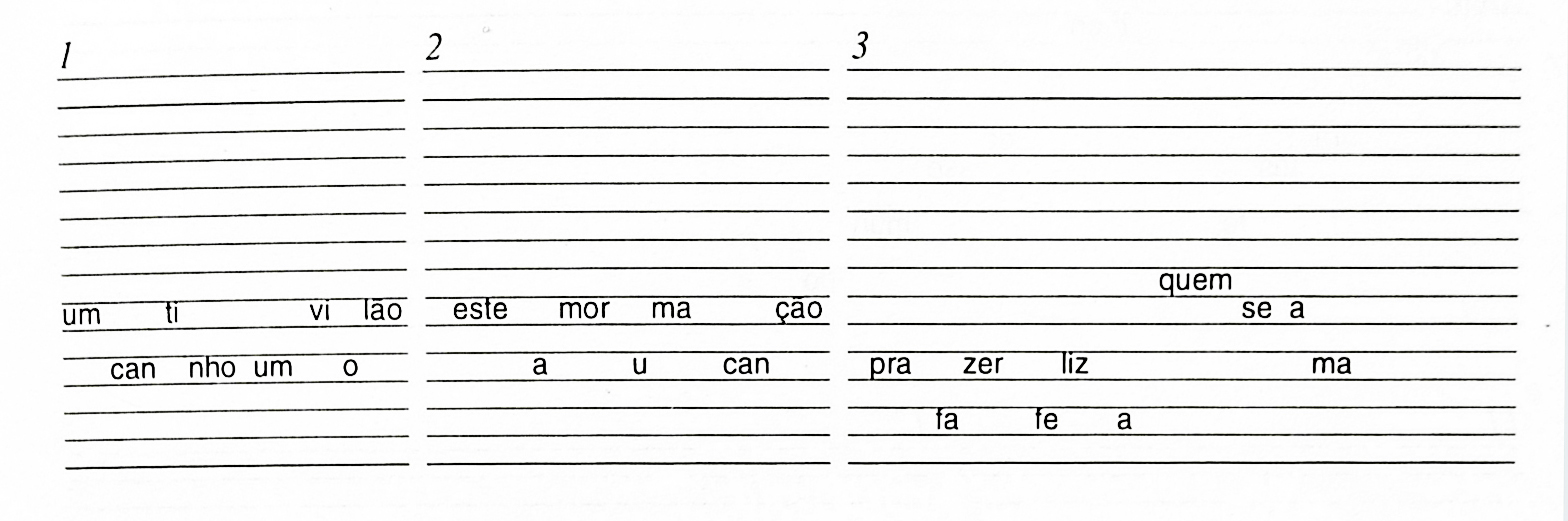
\includegraphics[width=\textwidth]{./imgs/figura1.jpg}

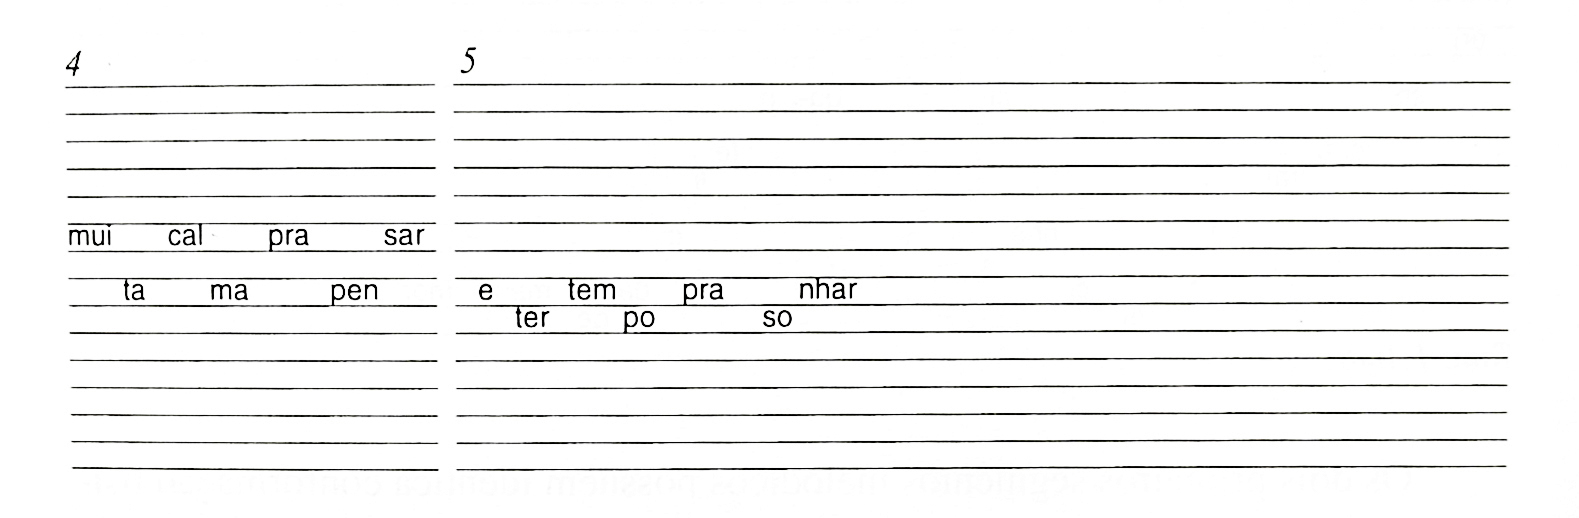
\includegraphics[width=\textwidth]{./imgs/figura2.jpg}
\end{figure}

\begin{figure}[H]
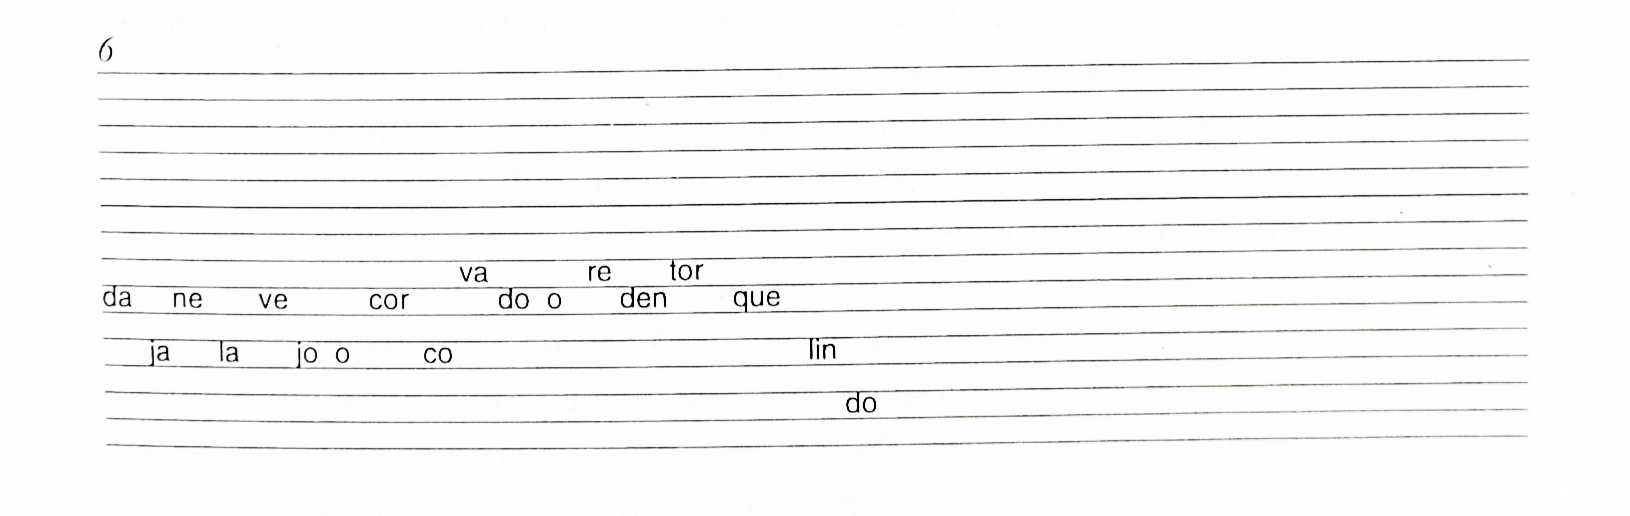
\includegraphics[width=\textwidth]{./imgs/figura3.jpg}

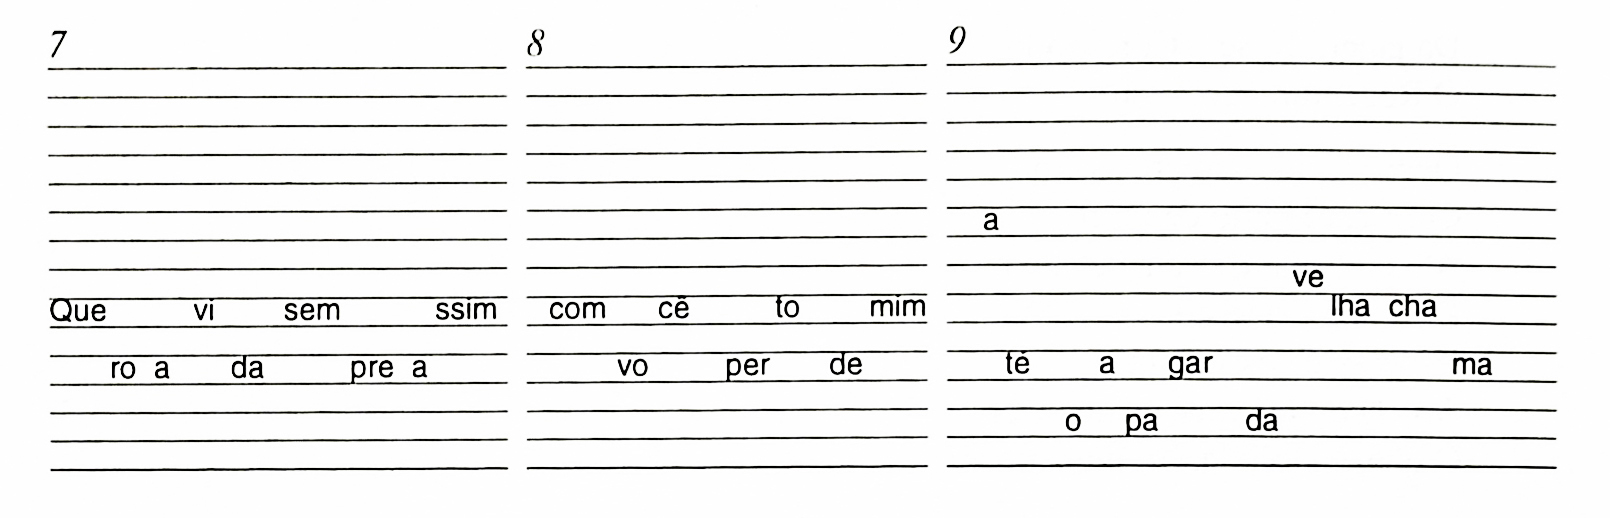
\includegraphics[width=\textwidth]{./imgs/figura4.jpg}

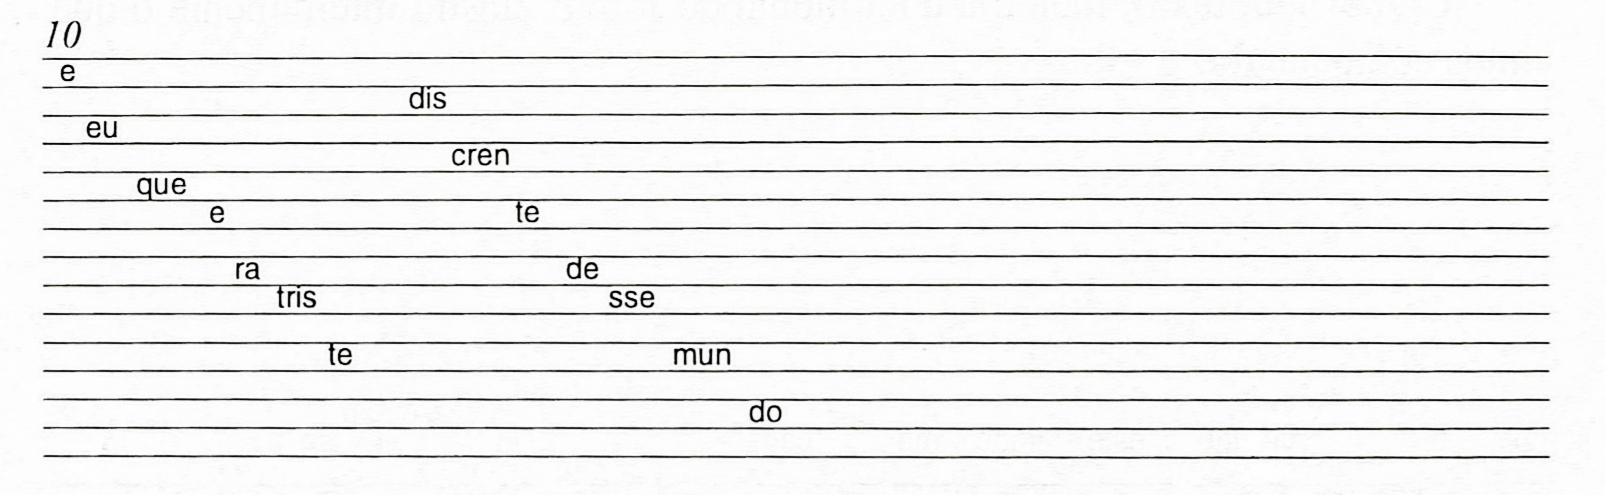
\includegraphics[width=\textwidth]{./imgs/figura5.jpg}

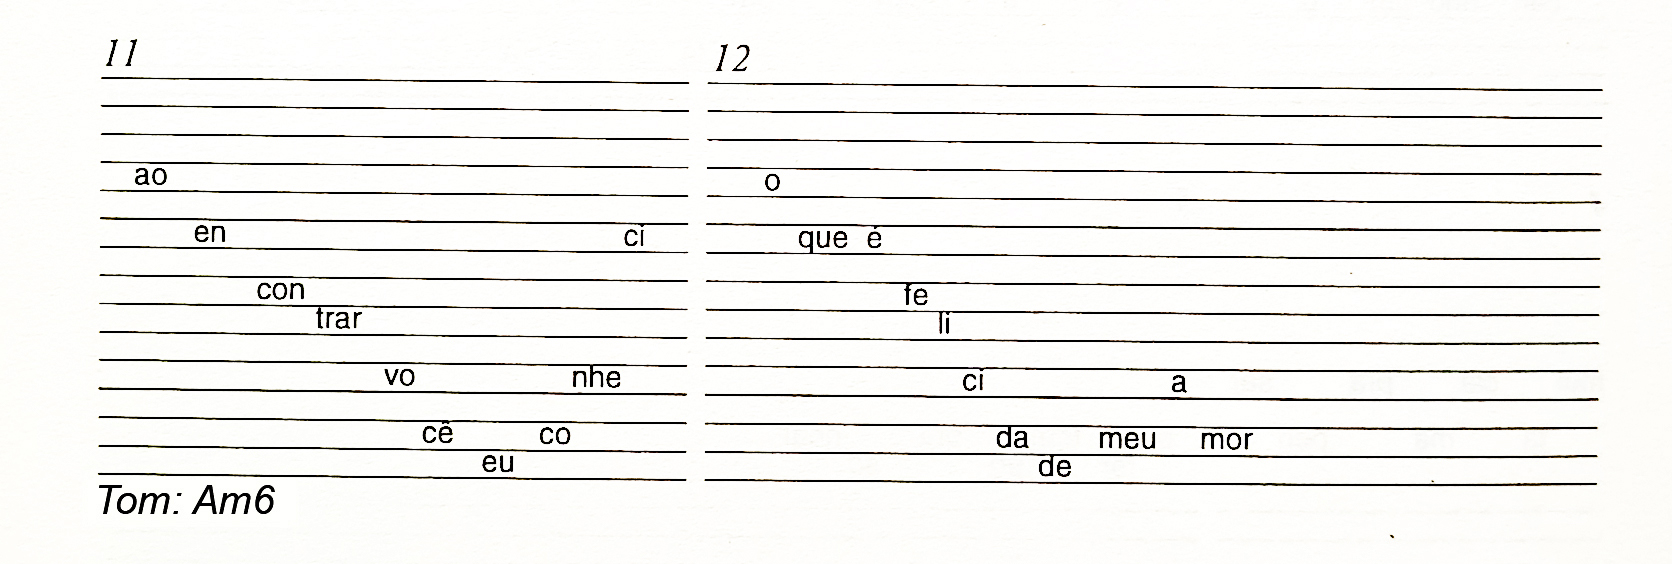
\includegraphics[width=\textwidth]{./imgs/figura6.jpg}
\end{figure}

Os dois primeiros segmentos melódicos possuem idêntica conformação
física, mas sentidos nitidamente inversos. Apesar de já termos um acorde
alterado Am6 na abertura, ainda não há diretividade suficiente para
canalizar sua força tensiva. Este acorde com esta melodia pode dar
sequência a inúmeras trajetórias perfeitamente integradas à sonoridade
inicial. A aplicação do segundo acorde Abº\,(b13), no início do
segmento seguinte, harmoniza a mesma melodia, mas engata um sentido
tensivo bem mais restritivo e acentuado.

Aqui cabe um esclarecimento harmônico. O acorde Abº\,(b13), tocado
isoladamente, é quase um ruído autônomo, muito menos definido, do ponto
de vista tonal, que o acorde anterior, Am6. No entanto, procedendo à
passagem deste último acorde ao seguinte, Gm7, adquire uma função ao
mesmo tempo ativa e retroativa. Ativa porque exerce forte tensão sobre
as principais notas que caracterizavam o acorde de Gm: a fundamental e
a terça (G Bg). O acorde de Ab\,(b13) contém as frequências Ab e
Cb (ou B), sensíveis superiores e, portanto, polarizadoras das
mencionadas notas, tensão que se acentua em virtude do movimento
cromático descendente desde o primeiro acorde. 

Na configuração invertida do violão:

\begin{figure}[H]
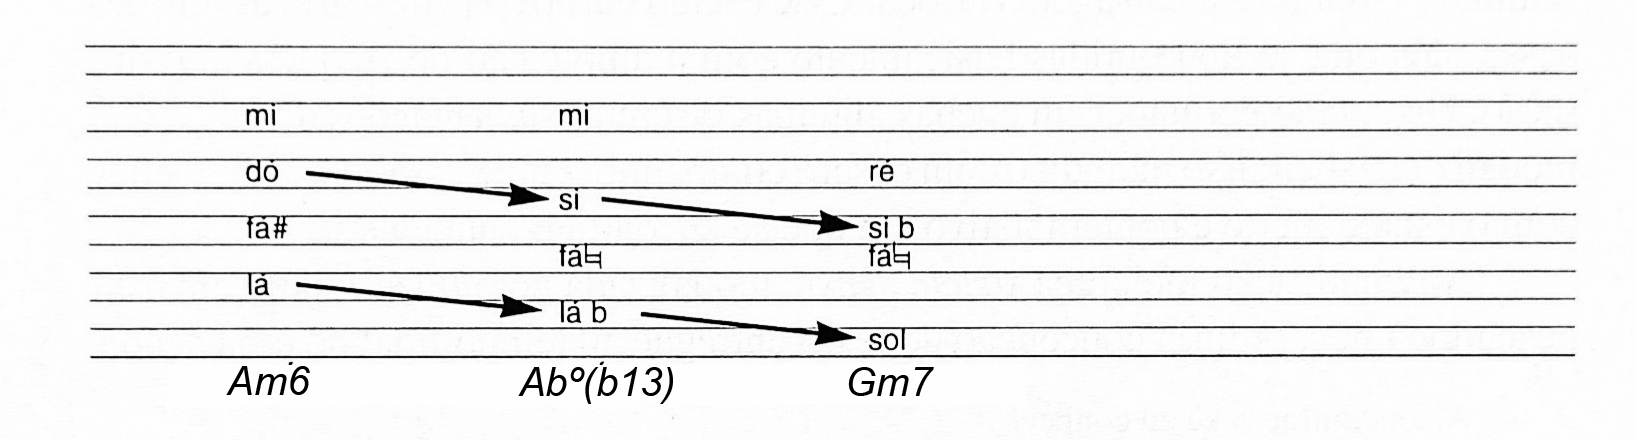
\includegraphics[width=\textwidth]{./imgs/figura7.jpg}
\end{figure}

Retroativa porque o sentido definido com esse segundo acorde determina
de vez a rota do primeiro, extraindo dele a função de simples dominante
(como se fosse um D7\,(9) preparando um G7\,(13).

Na verdade, toda a progressão musical, do primeiro ao terceiro segmento,
descreve uma trilha composta de sucessivas dominantes encadeadas que só
se distendem, temporariamente, ao atingir o acorde da \textsc{fm6} no final da
última sílaba deste trecho.

\begin{figure}[H]
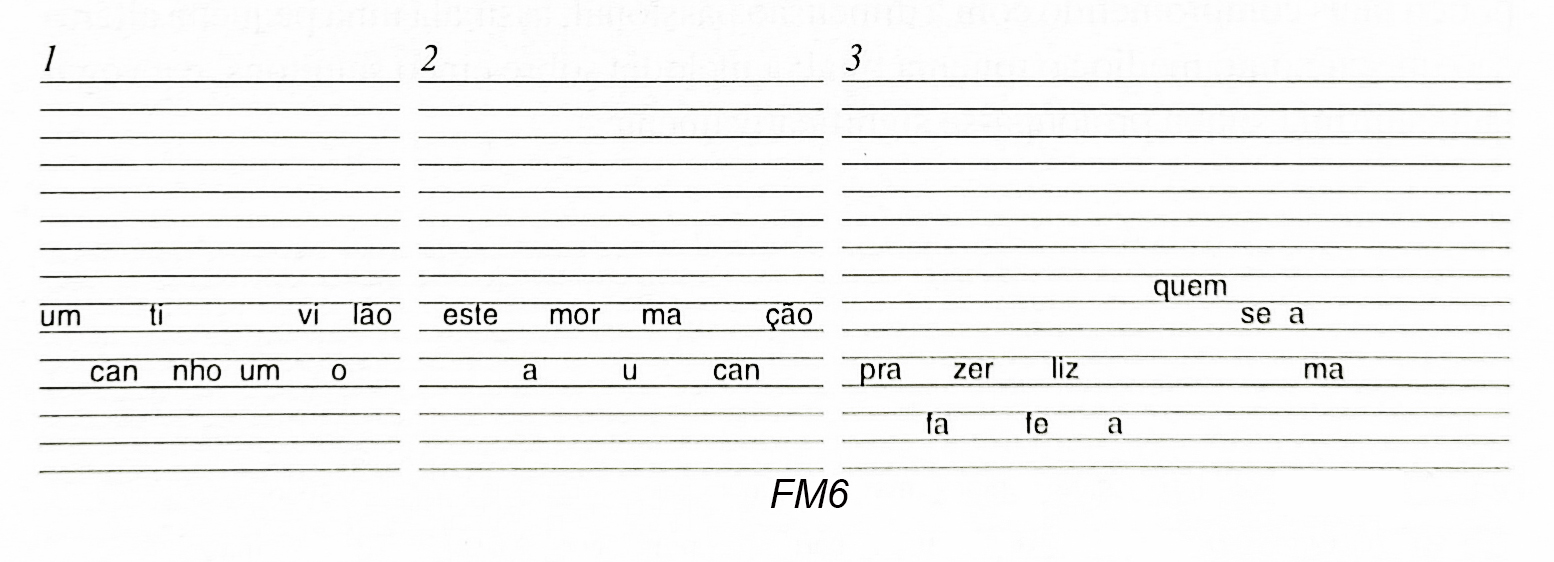
\includegraphics[width=\textwidth]{./imgs/figura8.jpg}
\end{figure}

Eis um percurso bem característico da bossa nova de Jobim. Trajetória
melódica quase sem variação, mas com o sentido palmilhadamente modulado
pela condução harmônica. Como se o acorde desbravasse o caminho e a
melodia apenas tomasse posse. Bem ao contrário da conduta anterior,
quando a função da harmonia era perseguir a melodia, livre nas
inflexões, mas totalmente subordinada aos roteiros fortemente
centrípetos da tonalidade --- podemos pensar no modelo de uma pajem que
acompanha a criança por onde ela for desde que não ultrapasse uma
pequena área prefixada.

Jobim conquista as novas zonas de sentido musical não com a melodia, mas
com a harmonia. À melodia da bossa nova sempre reservou um comportamento
reiterativo entre a tematização e a enumeração entoativa. A razão disso
pode ser encontrada, até certo ponto, em ``Corcovado.''

O texto desta canção retrata um estado final de conjunção plena com os
valores responsáveis por sua felicidade: \textit{cantinho}, \textit{violão}, \textit{amor},
\textit{canção}, \textit{calma}, \textit{sonho} e a \textit{paisagem carioca}. Esse estado eufórico já
descarta as tensões passionais que seriam obtidas basicamente com a
ampliação de frequência e duração. Da paixão permanecem apenas algumas
discretas sustentações de notas que modelizam o percurso melódico com o
\textit{ser}, compatibilizando essas desacelerações com o estado inerte e
contemplativo em que se encontra o enunciador.

A tematização melódica \textit{stricto sensu}, modalizada pelo \textit{fazer}, também
está descartada pela própria concepção do texto entregue ao tempo final
de uma ação:

\begin{verse}
\small{Ao encontrar você eu conheci\\
O que é felicidade meu amor}
\end{verse}

Nesse caso, como já vimos, a reiteração melódica está mais para a
enunciação entoativa que para os impulsos somáticos próprios do gênero.
É quando o motivo melódico se faz denominador comum dos valores, das
virtudes e dos desejos, reunidos todos na conjunção com o enunciador.

Nesse sentido, os dois primeiros segmentos, agregando valores de mesma
natureza no texto, repetem, na melodia, os mesmos motivos. O terceiro
segmento, um pouco mais comprometido com a dimensão passional, assinala
uma pequena alteração do seu ponto médio ao tonema final: a melodia
sobre cinco semitons, e a vogal da penúltima sílaba prolonga-se
significativamente.

\begin{figure}[H]
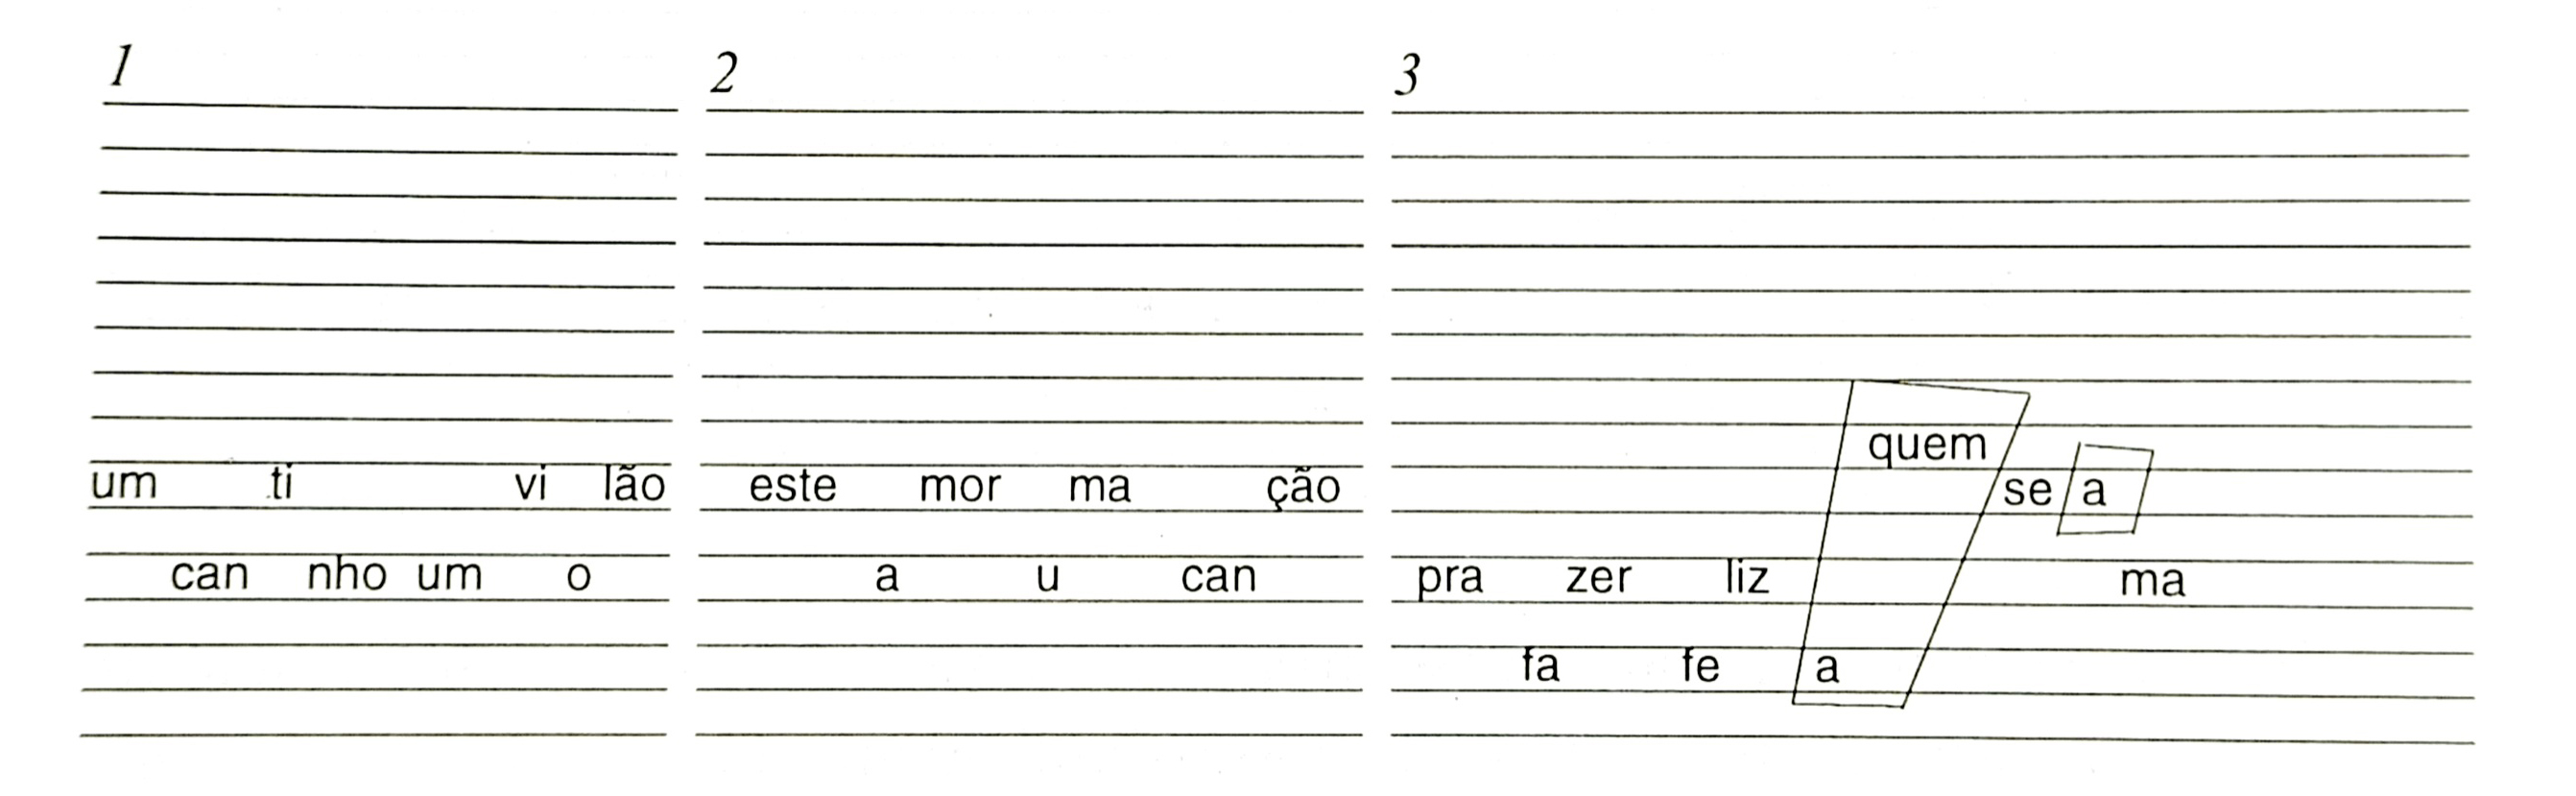
\includegraphics[width=\textwidth]{./imgs/figura10.jpg}
\end{figure}

Todo esse percurso, calcado numa linearidade fortemente reiterativa,
possui um sentido tão variado quanto lógico, assegurado pelas
intervenções ininterruptas da base harmônica. São seis acordes que
afetam o sentido das curvas. Ao mesmo tempo que buscam a conclusão
parcial, suas dissonâncias vão aclimatando a progressão melódica e
substituindo, qualitativamente, as tensões evitadas nos contornos.
Exemplo típico é o acorde de Fº que acompanha a duração da penúltima
sílaba \textit{a} (em \textit{ama}). É a tensão linear da melodia condensada na
densidade dominante do acorde. Com isso eliminam-se exageros passionais,
mantendo um nível de tensão emotiva controlado mais pelos recursos
musicais do que pela espontaneidade entoativa.

Essa foi uma das grandes recuperações da bossa nova, numa época em que o
derramamento passional de melodia imperava nas rádios. Jobim recolheu as
tensões dos contornos e condensou-as nos acordes. Podia, então, evitar
os excessos suspeitos que rondavam as inflexões, bastando para isso um
bom aproveitamento do sentido melódico já conduzido pela harmonia.

``Corcovado'' segue seu devenir mantendo a mesma conduta, com seus motivos
reiterando ora pouco mais acima, ora pouco mais abaixo, mas sempre sob a
determinação dos acordes alterados, até que a primeira parte se
interrompe com uma figura exclamativa.

\begin{figure}[H]
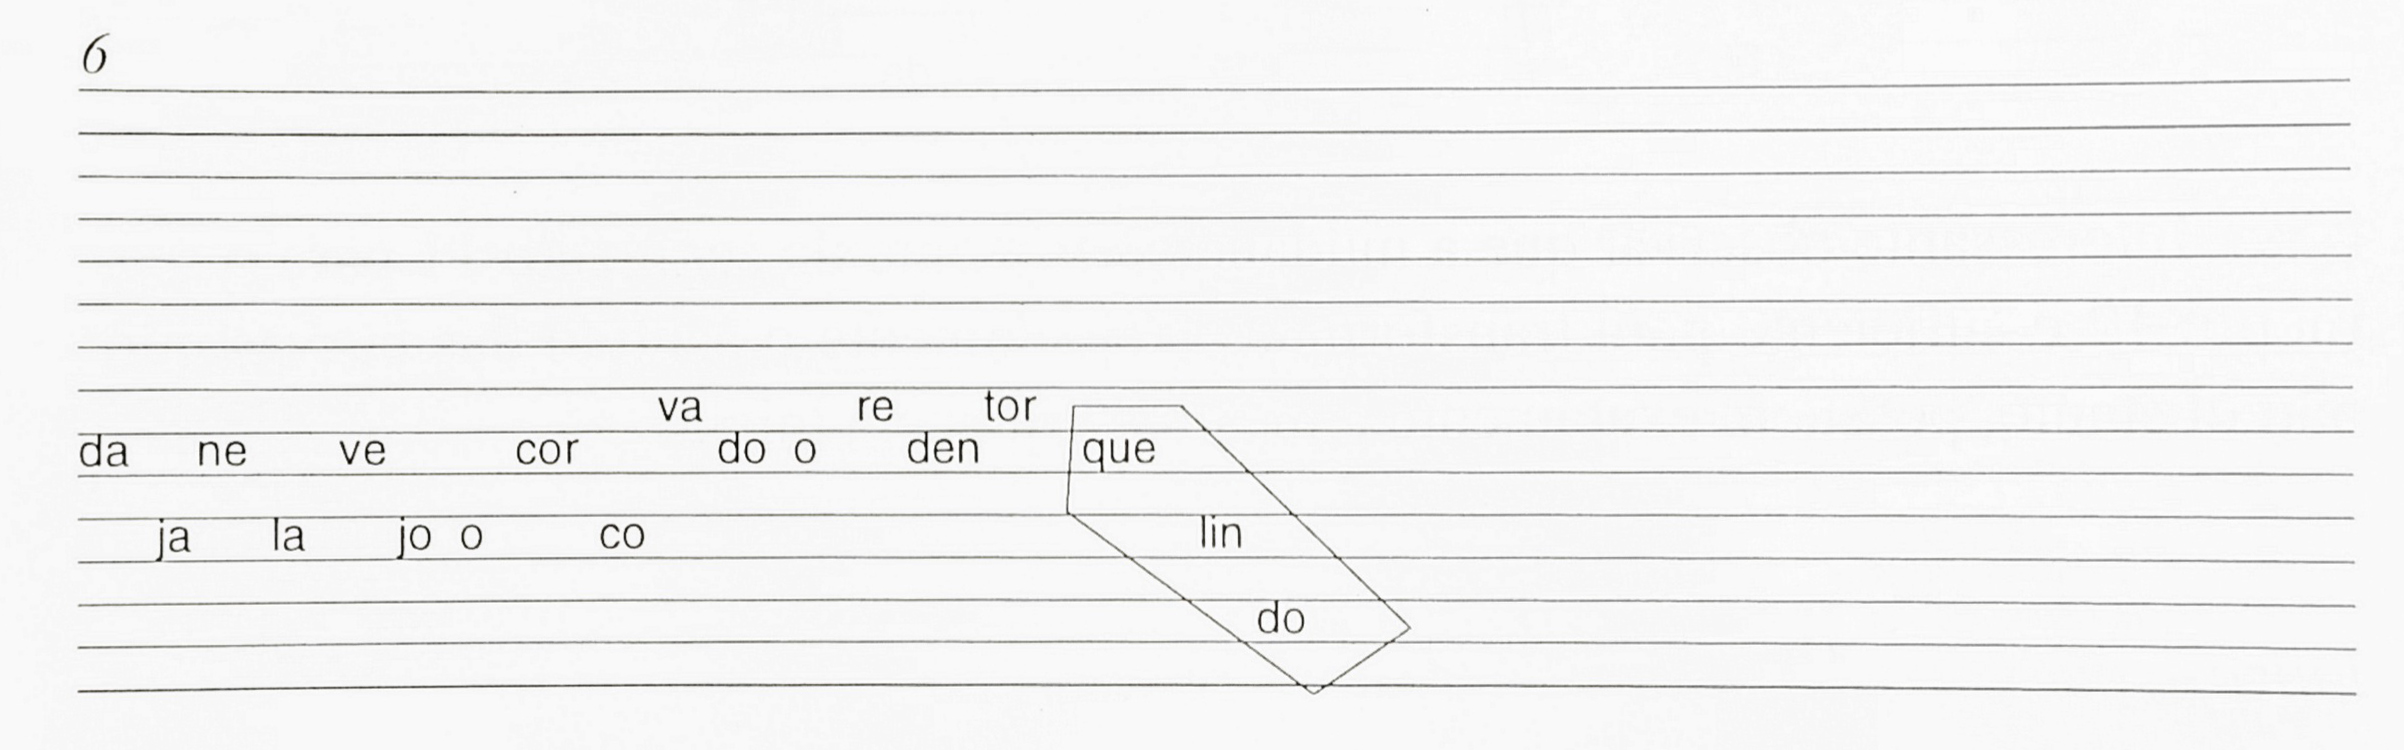
\includegraphics[width=\textwidth]{./imgs/figura11.jpg}
\end{figure}

É um breve extravasamento da enunciação cuja moderação também faz parte
da dicção de Jobim.

Do segmento \textsc{vii} ao \textsc{xix} temos a repetição melódica dos segmentos \textsc{i}, \textsc{ii} e \textsc{iii} com
uma versão de letra bastante próxima à primeira.

Somente à altura do décimo segmento vamos encontrar uma modificação do
esquema melódico que coincide com a mudança do registro linguístico.
Sobre acordes bem semelhantes aos da primeira parte, a melodia se
reveste de tensão passional e descreve amplas progressões descendentes,
ao mesmo tempo que o texto relata uma fase anterior, marcada pela
disjunção efetiva.

\begin{figure}[H]
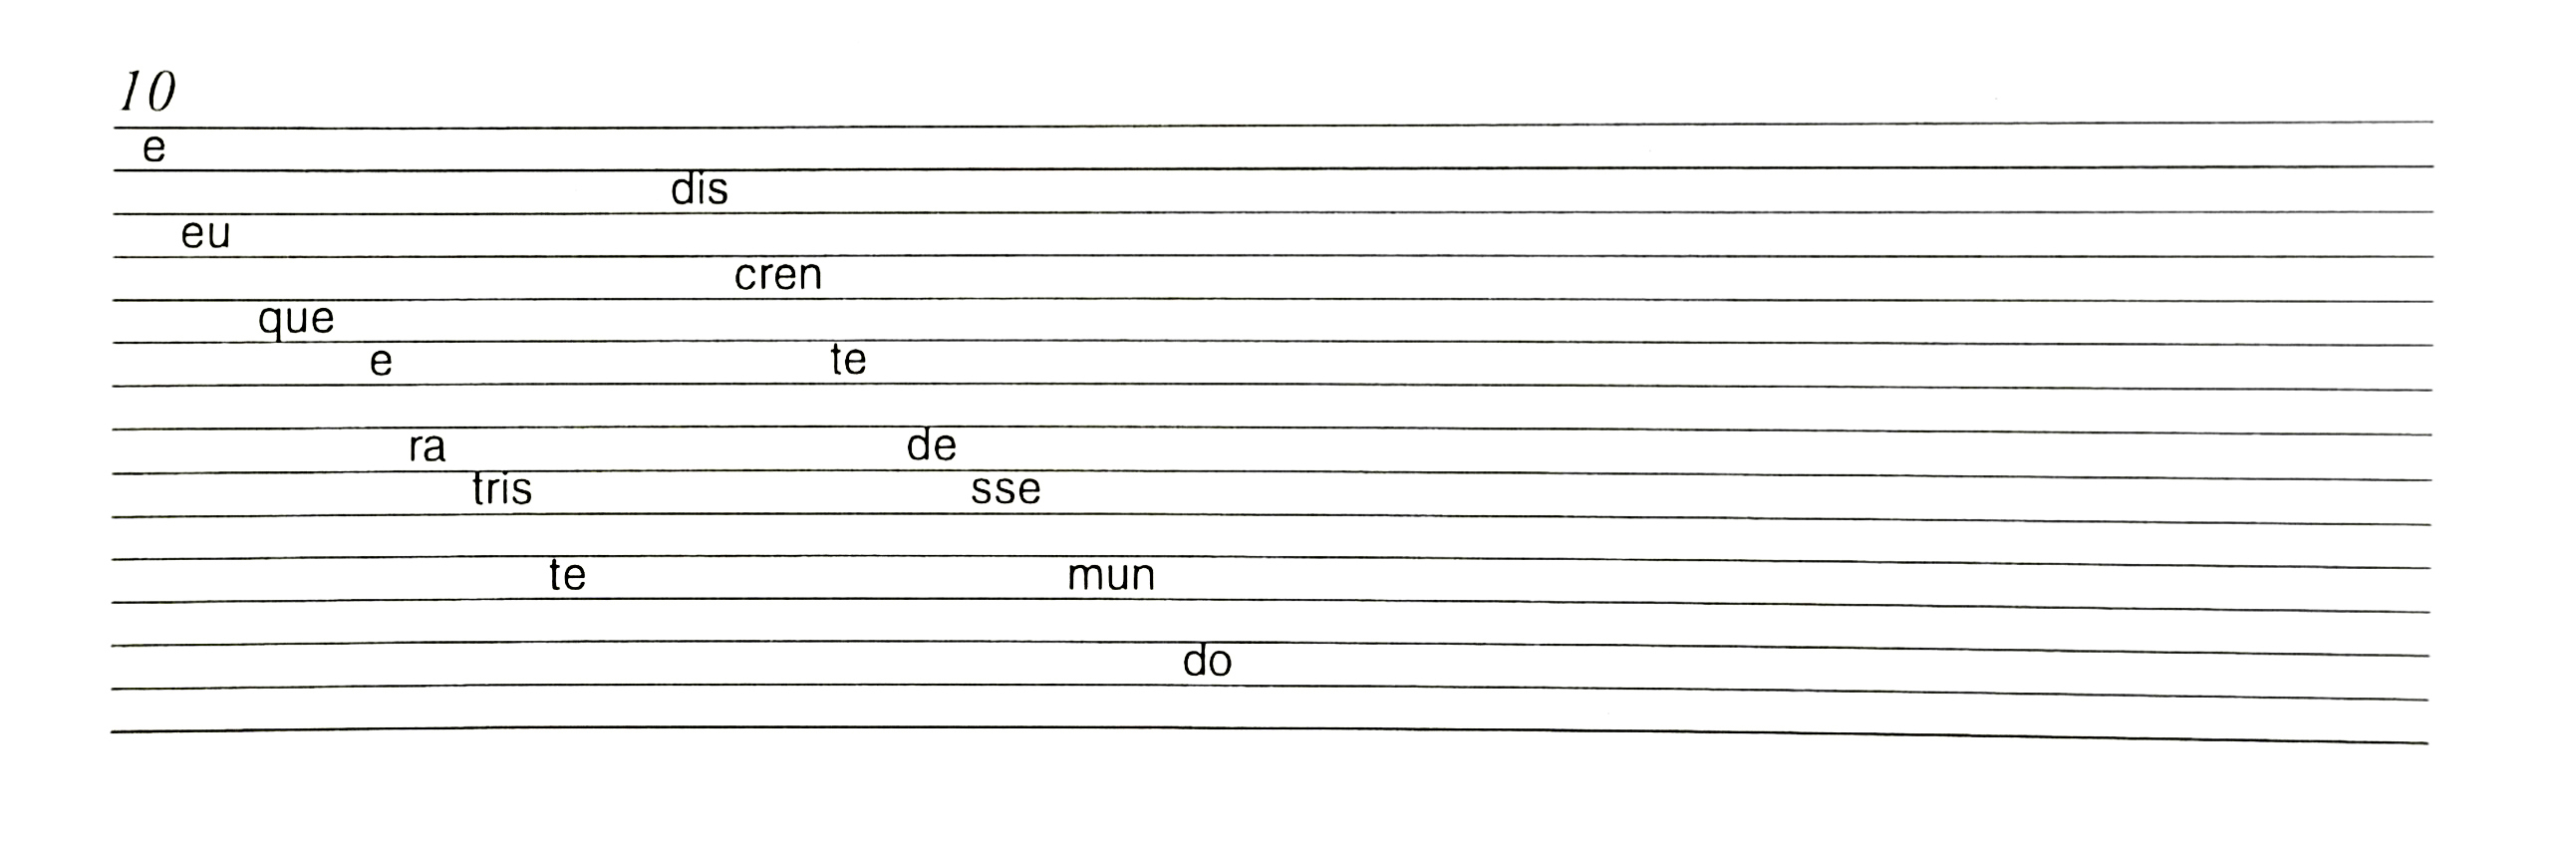
\includegraphics[width=\textwidth]{./imgs/figura12.jpg}
\end{figure}

No segmento \textsc{xi}, a curva já adquire um sentido continuativo com a mudança
de rota ocasionada pelo tonema ascendente, contrastando e se
complementando com a descendência do último segmento, que ratifica o
estado conjuntivo pelo qual toda a composição se pautou.

\begin{figure}[H]
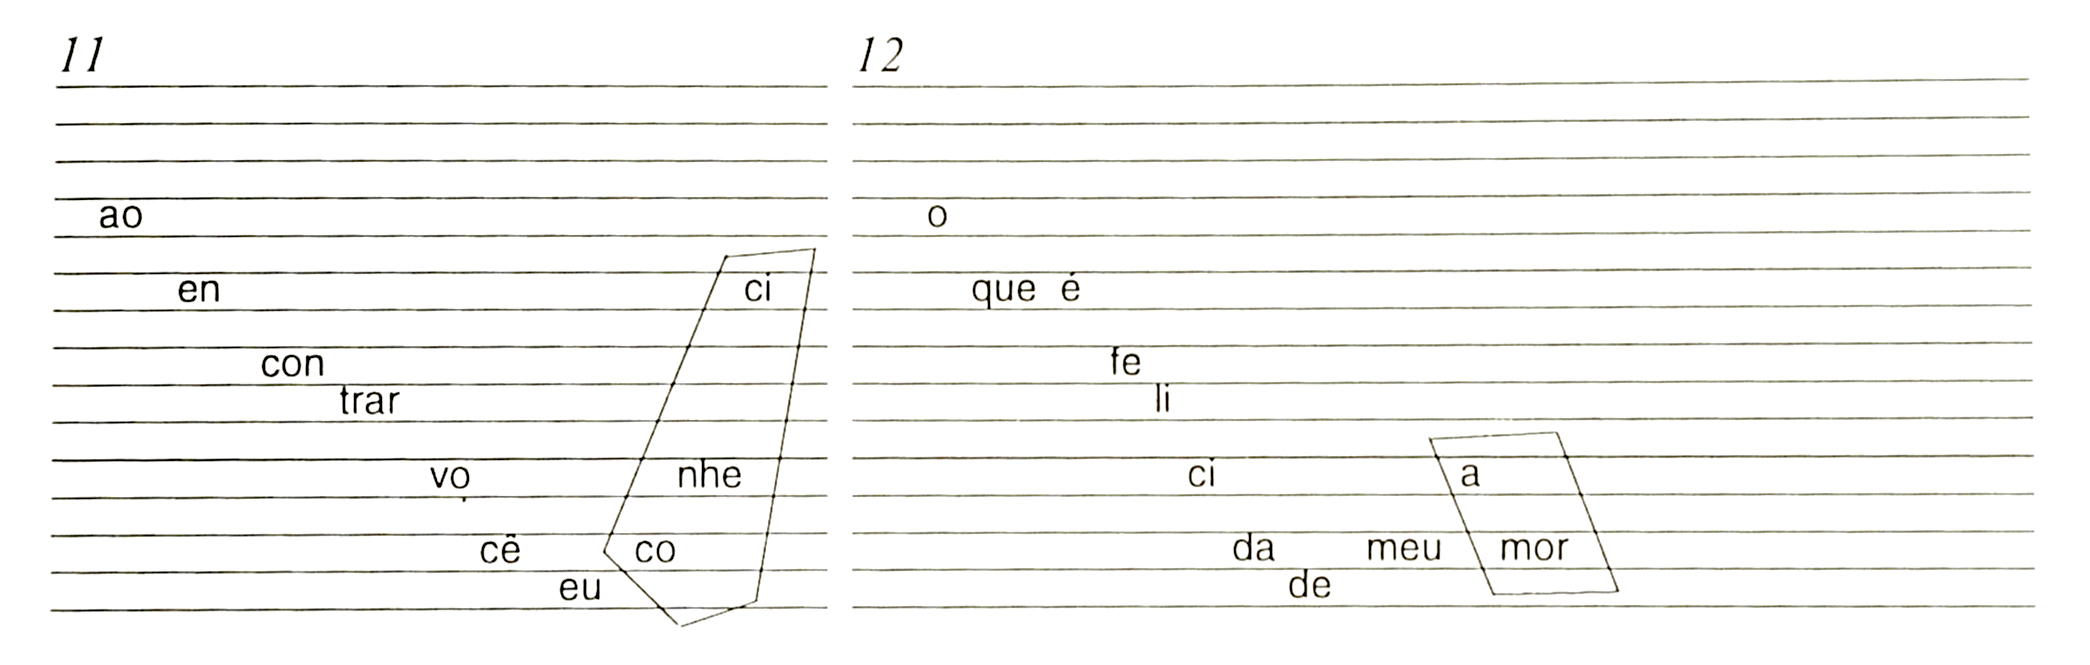
\includegraphics[width=\textwidth]{./imgs/figura13.jpg}
\end{figure}

Interessante observar que a mudança de tonema do segmento \textsc{xi} para o
segmento \textsc{xii} é suficiente para transformar completamente o sentido das
curvas que, não obstante, possuem exatamente a mesma sequência inicial.

\begin{verse}
\small{Luiza\\
Rua, espada nua\\
Bóia no céu imensa e amarela\\
Tão redonda a lua\\
Como flutua\\
Vem navegando\\
O azul do firmamento\\
E no silêncio lento\\
Um trovador, cheio de estrelas\\
Escuta agora a canção que eu fiz\\
Pra te esquecer, Luiza\\
Eu sou apenas um pobre amador\\
Apaixonado\\
Um aprendiz do teu amor\\
Acorda amor\\
Que eu sei que embaixo desta neve\\
Mora um coração\\
Vem cá, Luiza\\
Me dá tua mão\\
O teu desejo é sempre o meu desejo\\
Vem, me exorciza\\
Me dá tua boca\\
E a rosa louca\\
Vem me dar um beijo\\
E um raio de sol\\
Nos teus cabelos\\
Como um brilhante que partindo a luz\\
Explode em sete cores\\
Revelando então os sete mil amores\\
Que eu guardei somente\\
Pra te dar, Luiza}
\end{verse}

Resumo aqui as três funções principais do acorde dissonante na dicção de
João Gilberto e Tom Jobim, na fase da implantação da bossa nova:

\begin{itemize}
\item
  Agente modalizador do sentido (direção) melódico;
\item
  Agente condensador da tensão passional;
\item
  Caracterização de uma totalidade compacta apropriada para a batida
  rítmica regular.
\end{itemize}

A primeira compreende as operações de desengate e engate que transformam
o sentido subjacente da rota do continuum melódico. A segunda função é
aquela que transfere para dentro do acorde as tensões de frequência,
substituindo o esforço de emissão pelas tensões de polarização tonal. A
última função, por fim, corresponde ao uso do acorde cristalizado como
instrumento de percussão. Daqui sai o samba estilizado em bossa nova.

Essas funções contribuem para a invenção de melodias reiterativas e
pouco expansivas no campo da tessitura. Presumível, uma vez que o
sentido melódico passa a depender menos das inflexões em si e as
matrizes rítmicas se configuram melhor com a repetição de seus motivos.
A bossa nova se torna, assim, um movimento musical que culpa o próprio
gênero como fase de dicção. Imperam as tematizações ou as entoações
enumerativas. Os conteúdos disfóricos, que poderiam implicar grandes
desvios de curva melódica, são tratados quase esquematicamente, não como
experiência revivida no canto, mas como recurso expressivo, uma espécie
de ornamentação para produzir encanto.

A esquematização dos recursos persuasivos --- tematização, passionalização
e figurativização --- atingiu um tal grau de controle e de funcionalidade
estética que uma canção como ``Garota de Ipanema'' pôde ser concebida em
termos de oposição absoluta entre tematização e passionalização, uma
regendo a primeira parte e a outra, a segunda:

\subsection{primeira parte: tematização}

\begin{figure}[H]
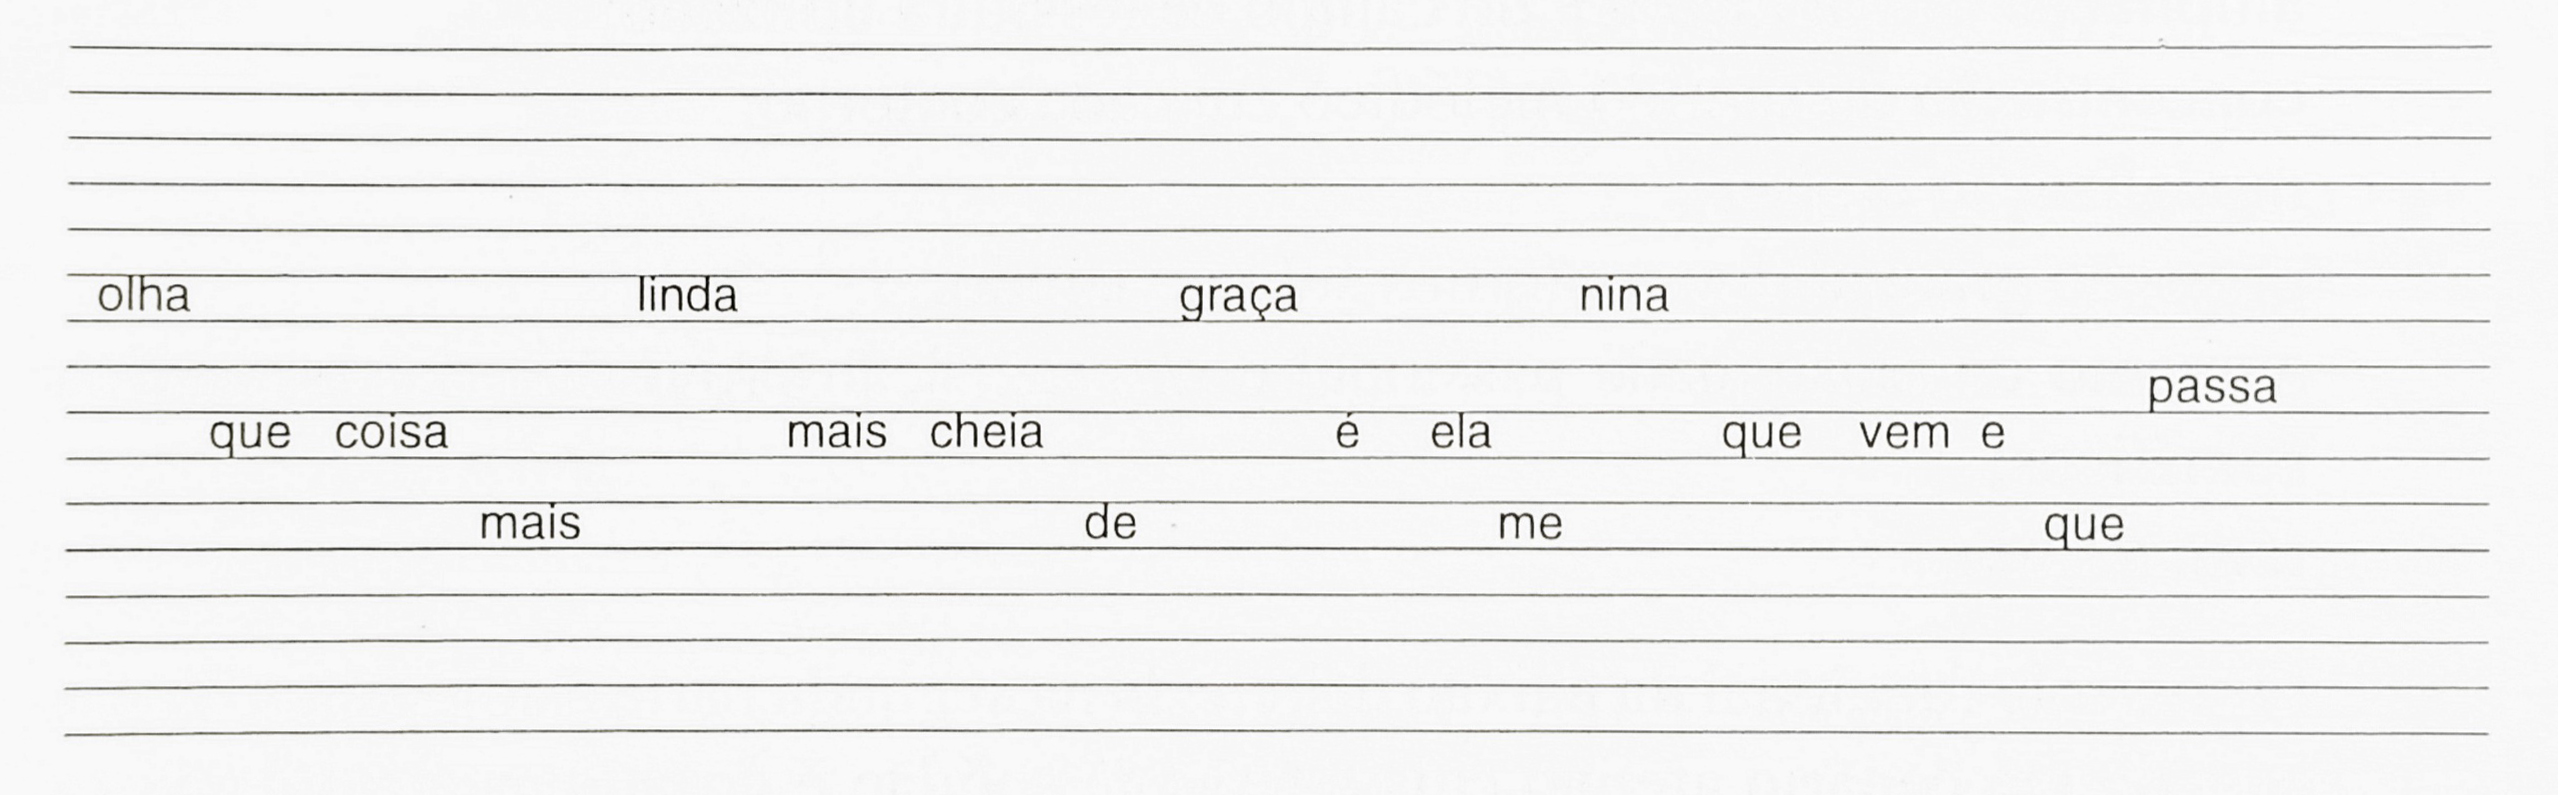
\includegraphics[width=\textwidth]{./imgs/figura14.jpg}
\end{figure}

\subsubsection{Texto} 
\begin{itemize}
\item Qualificação da ``Garota de Ipanema'', caracterizando sua maneira de ser, de
agir e sua capacidade de produzir fascínio;
\item Enunciador em estado de conjunção com os valores visuais;
\item Valorização dos ataques consonantais e dos acentos vocálicos.
\end{itemize}

\subsubsection{Melodia}
\begin{itemize}
\item Reiteração perseverante do motivo engendrando uma configuração temática
que ecoa o investimento temático da \textit{garota};
\item Modalização do \textit{fazer};
\item Tensividade somática produzida pela pulsação extremamente regular e
marcada;
\item Tom: \textsc{cm}.
\end{itemize}

\subsection{segunda parte: passionalização}

\begin{figure}[H]
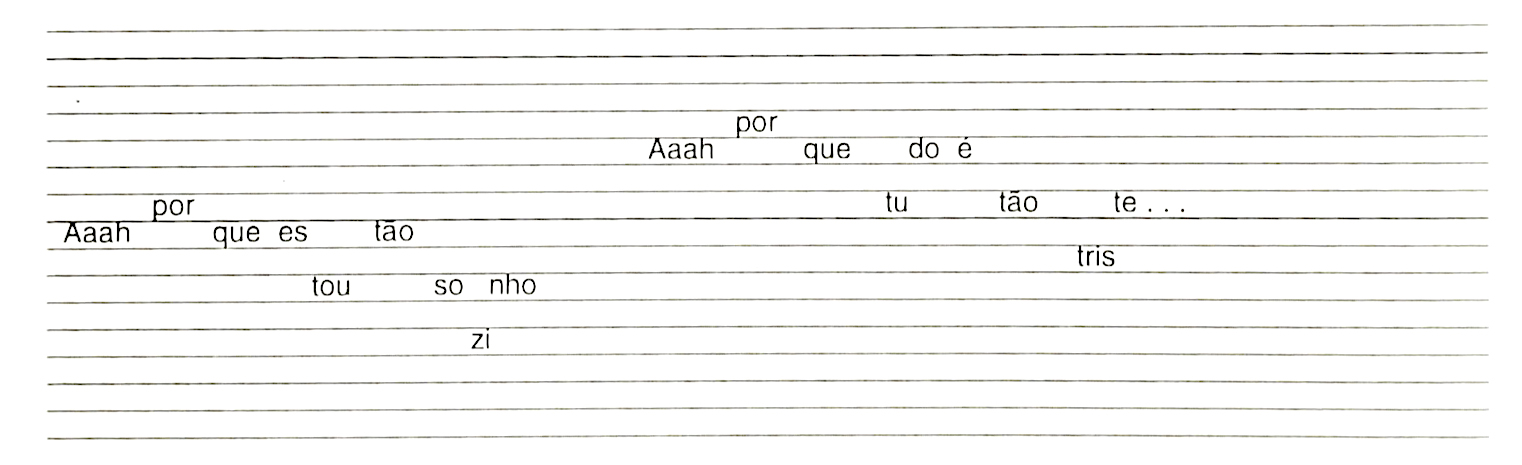
\includegraphics[width=\textwidth]{./imgs/figura15.jpg}
\end{figure}

\subsubsection{Texto}
\begin{itemize}
\item Focalização de um estado interno passivo e disfórico;
\item Enunciador em disjunção afetiva;
\item Interjeições lamuriosas;
\item Valorização dos prolongamentos vocálicos.
\end{itemize}

\subsubsection{Melodia}
\begin{itemize}
\item Ampliação das durações e do campo de tessitura utilizado;
\item Concentração do sentido melódico em cada contorno;
\item Modalização do \textit{ser};
\item Projeção gradual dos contornos sobre o agudo;
\item Aumento de tensividade passional e neutralização provisória dos estímulos somáticos;
\item Tom: D\,bM.
\end{itemize}

O controle funcional da paixão delineada na segunda parte é completo.
Trata-se apenas de um cenário afetivo cuja tensão de solidão é dosada na
medida exata de anseio pela garota. O sentimento de falta é o fundo para
fazer a figura da garota brilhar.

A bossa nova suprime o compromisso existencial com a paixão, assumindo
apenas seu valor estético como um recurso a mais para acariciar o belo.
A bossa nova legítima nunca abdicou do sonho: \textit{nem do amor, nem do
sorriso, nem da flor}. Seu controle dos recursos técnicos era apenas o
resultado de um domínio total da linguagem. João Gilberto e Tom Jobim
tiveram, naquele momento, a canção brasileira nas mãos. Debulharam-na e
mostraram a medula.

Essas marcas essenciais do movimento permaneceram de forma diluída ou
fragmentada em toda a música popular contemporânea. João Gilberto
aprofunda cada vez mais sua análise interpretativa da canção brasileira
com a radicalidade de um mito que já tem seu lugar plenamente
assegurado. Jobim retomou algumas vezes aqueles traços essenciais da
primeira hora e produziu novas obras-primas do gênero, como ``Águas de
Março'', por exemplo, já na década de 1970.

Entretanto, Jobim, como compositor, fez incursões por outros estilos que
nem sempre mantiveram o despojamento e a economia textual e melódica da
bossa nova. Um deles, por exemplo, beirou a experiência épica, inspirada
nas aventuras linguísticas de Guimarães Rosa: ``Matita Perê'', disco e
música. Outro, mais próximo do mercado, deu origem a algumas valsas
veiculadas pelo cinema e pela televisão: ``Tema de amor de Gabriela'' e
``Luiza.''

\begin{figure}[H]
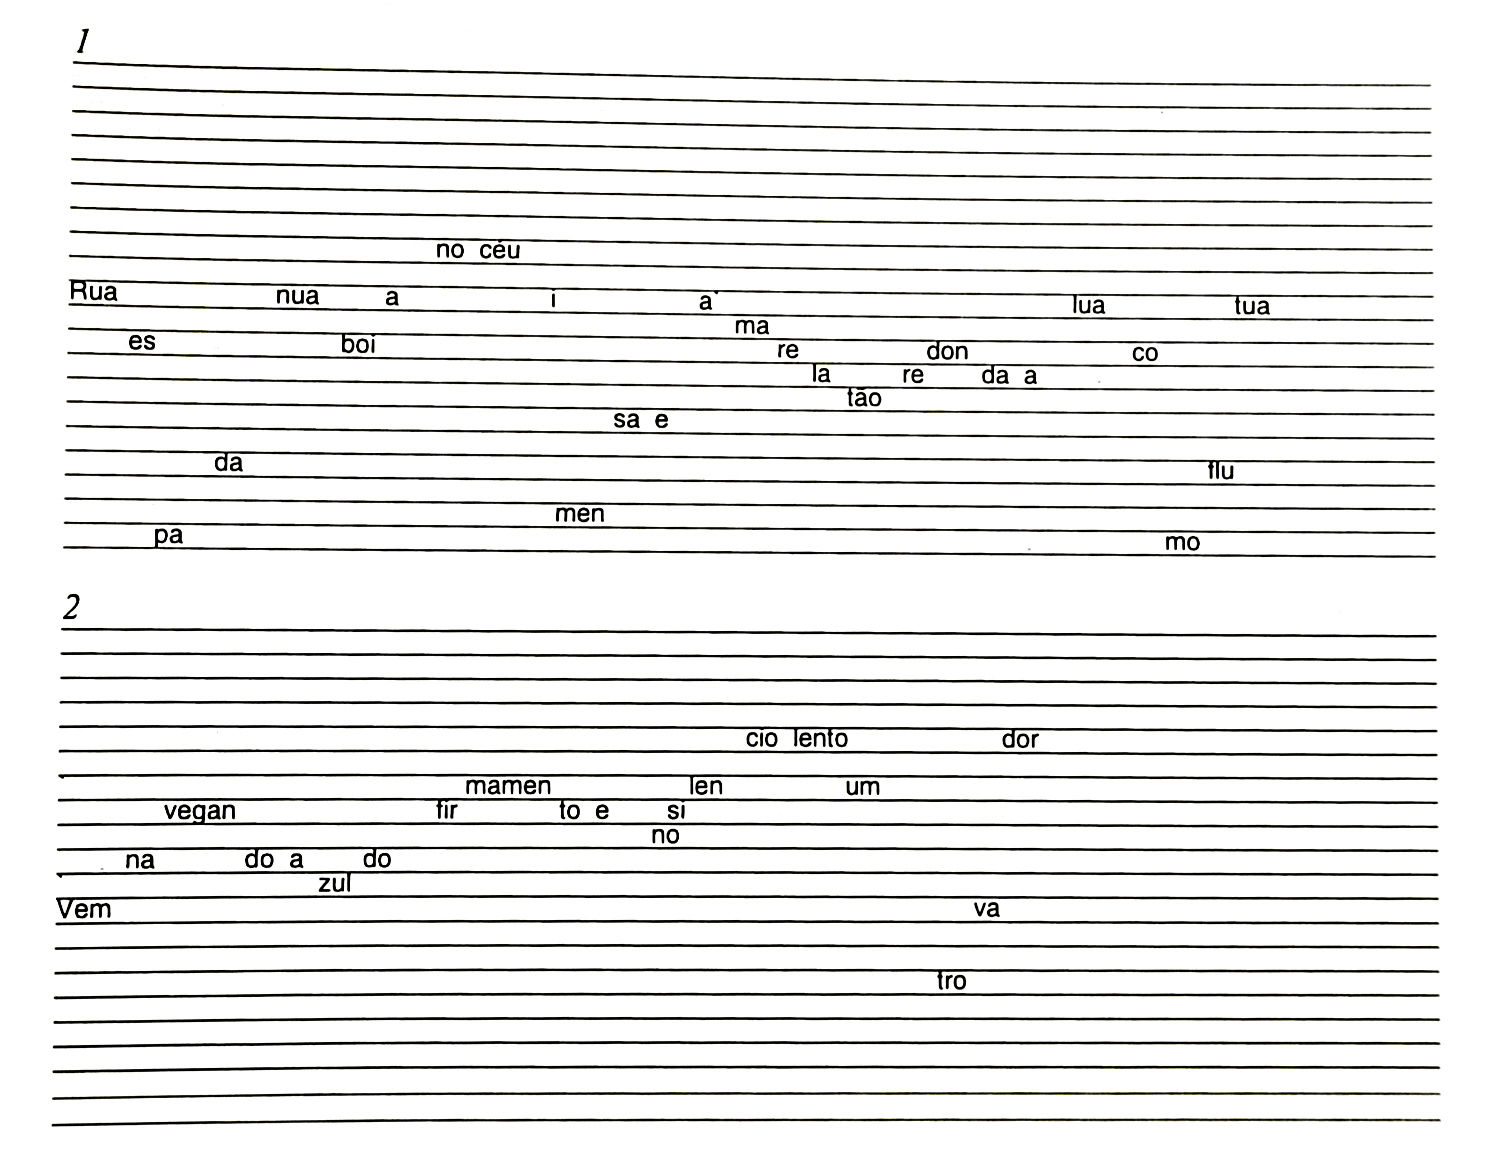
\includegraphics[width=\textwidth]{./imgs/figura16.jpg}
\end{figure}

\begin{figure}[H]
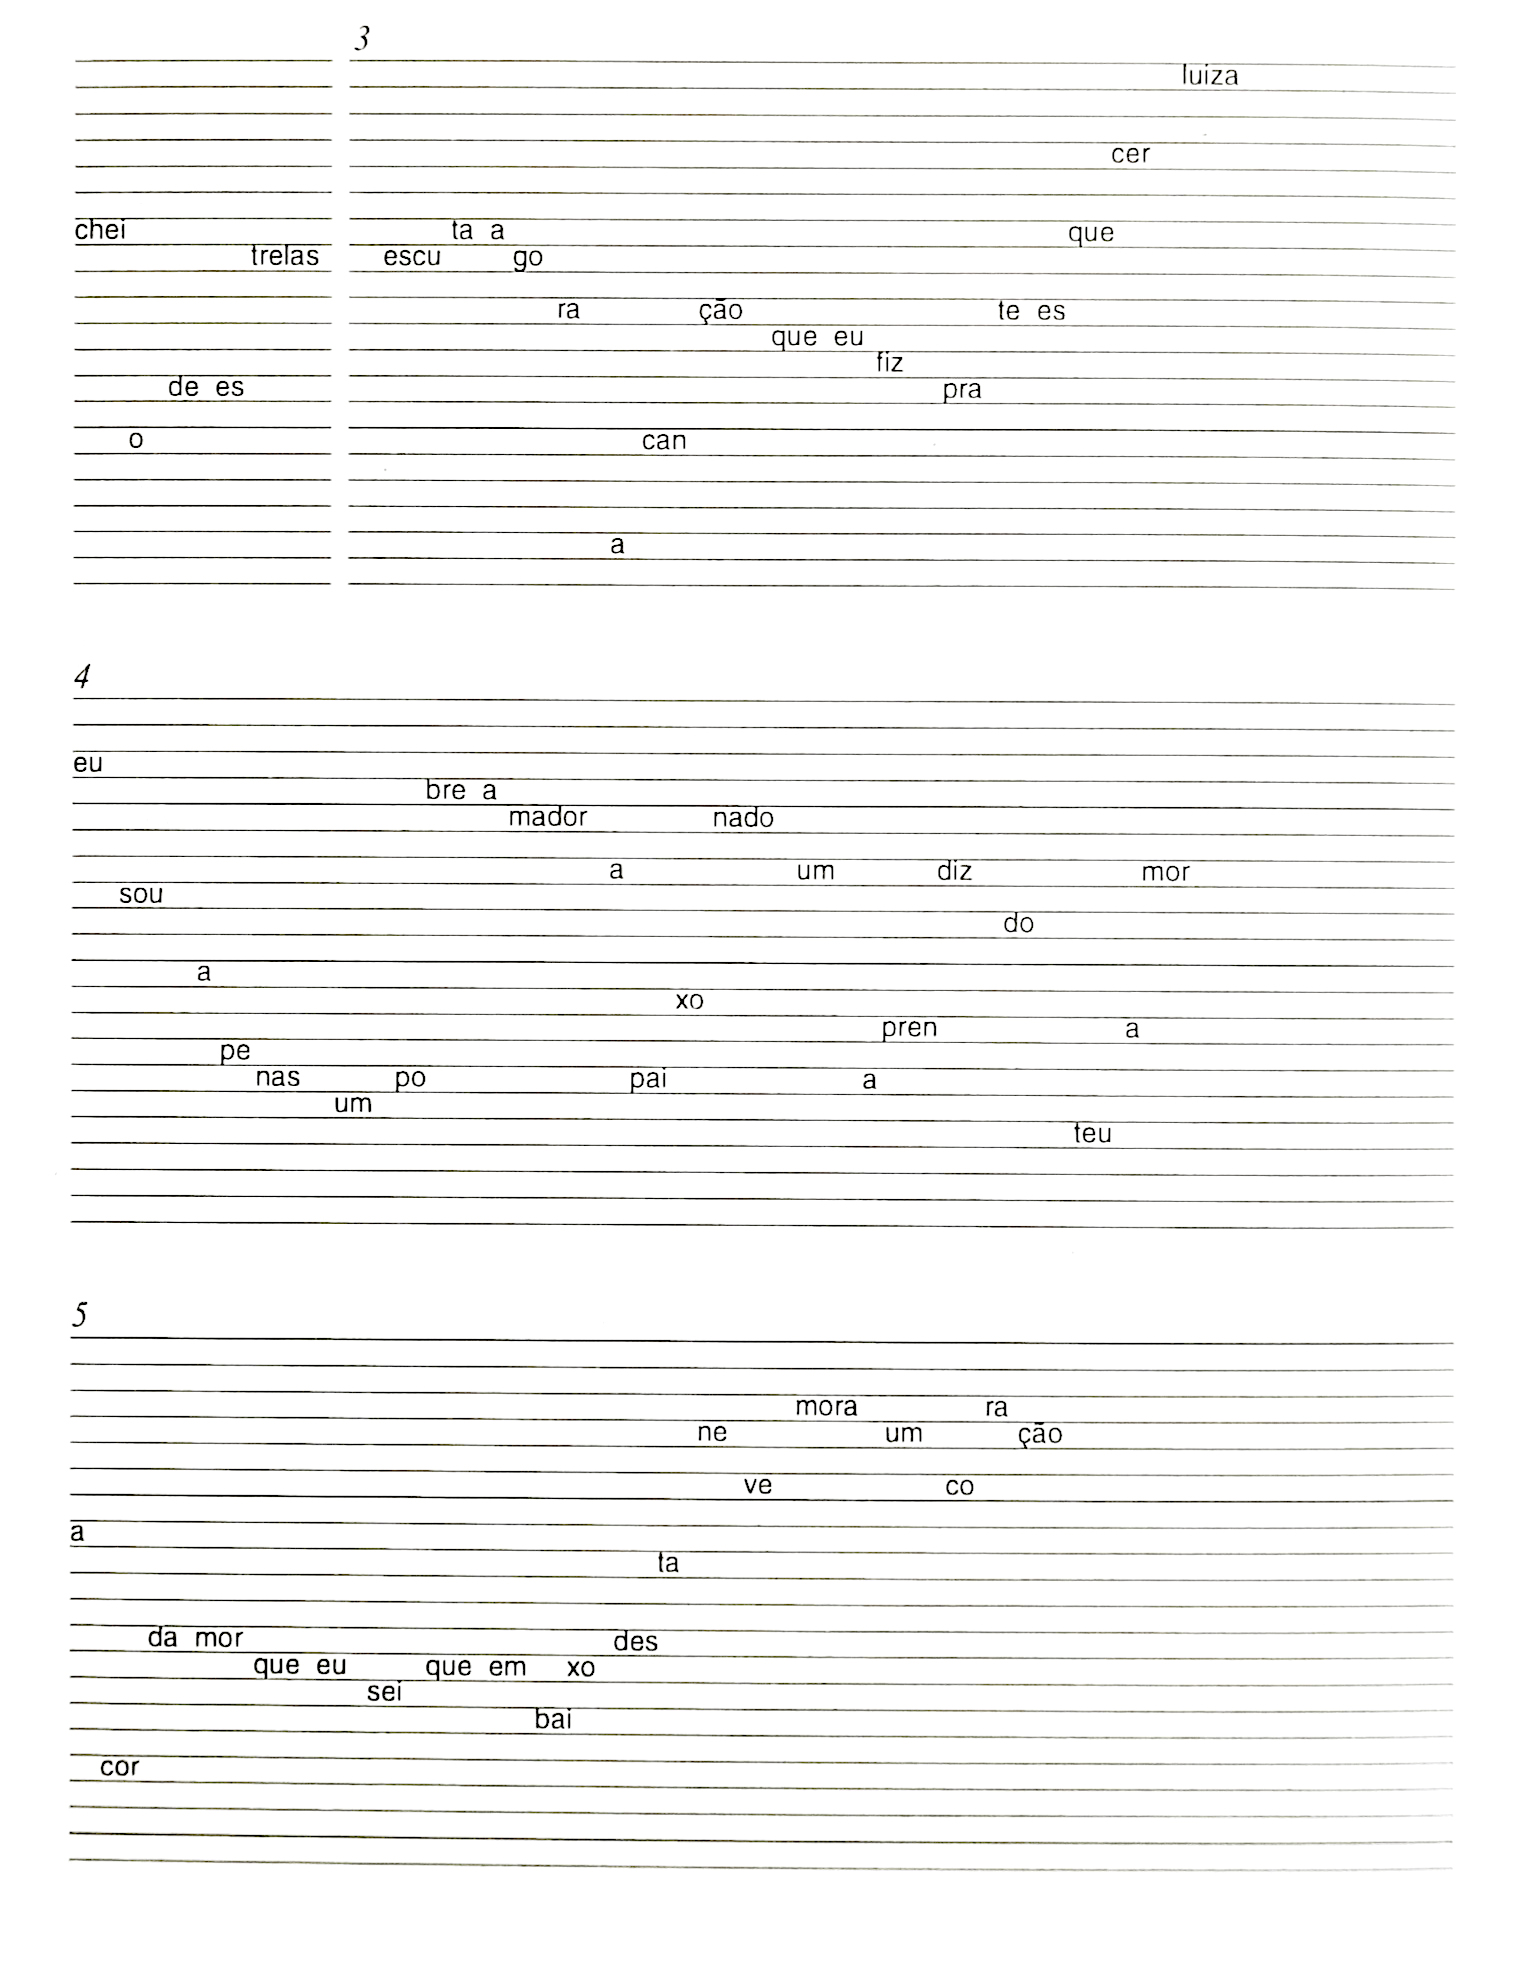
\includegraphics[width=\textwidth]{./imgs/figura17.jpg}
\end{figure}

\begin{figure}[H]
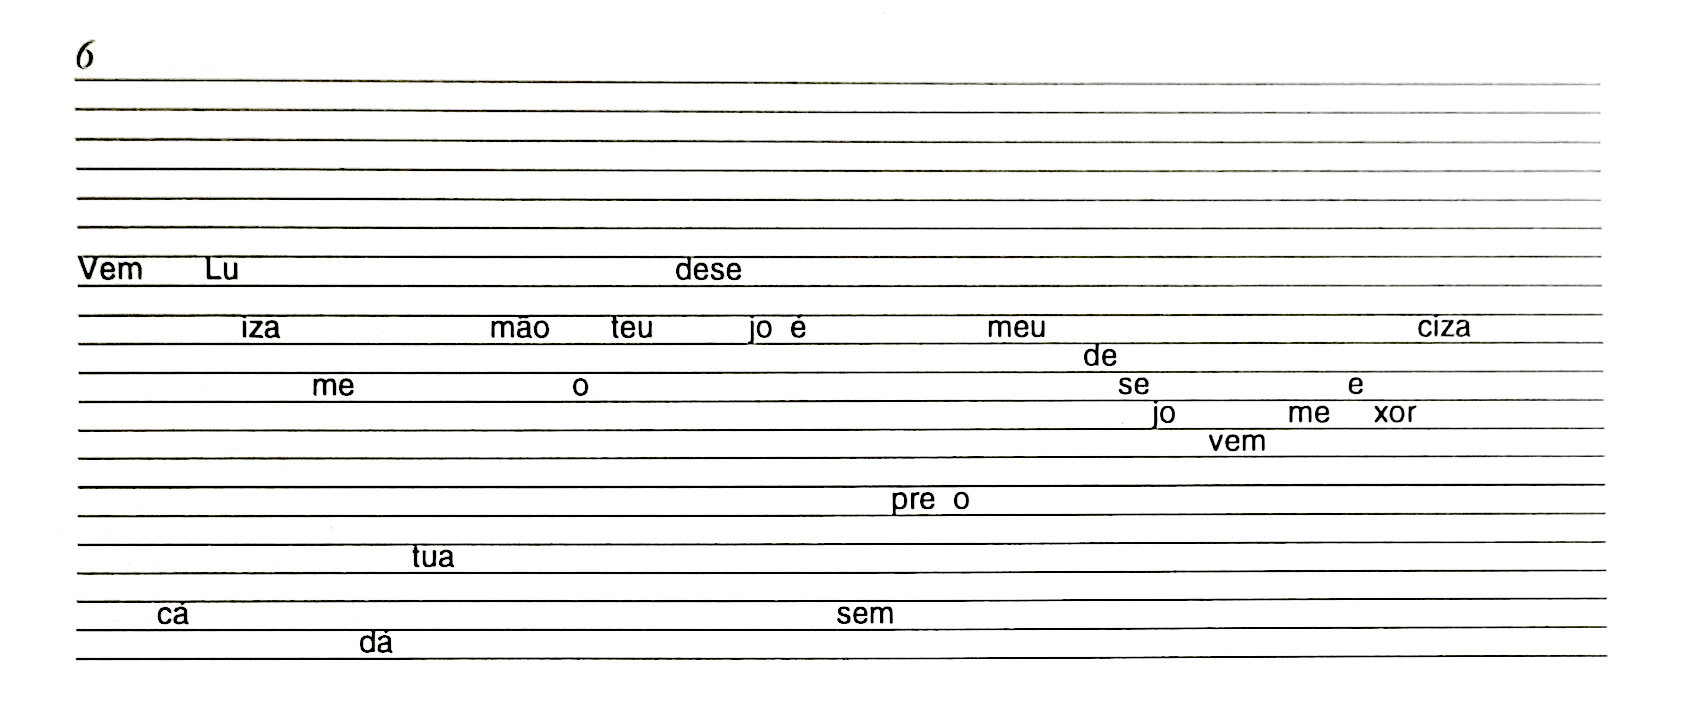
\includegraphics[width=\textwidth]{./imgs/figura18.jpg}

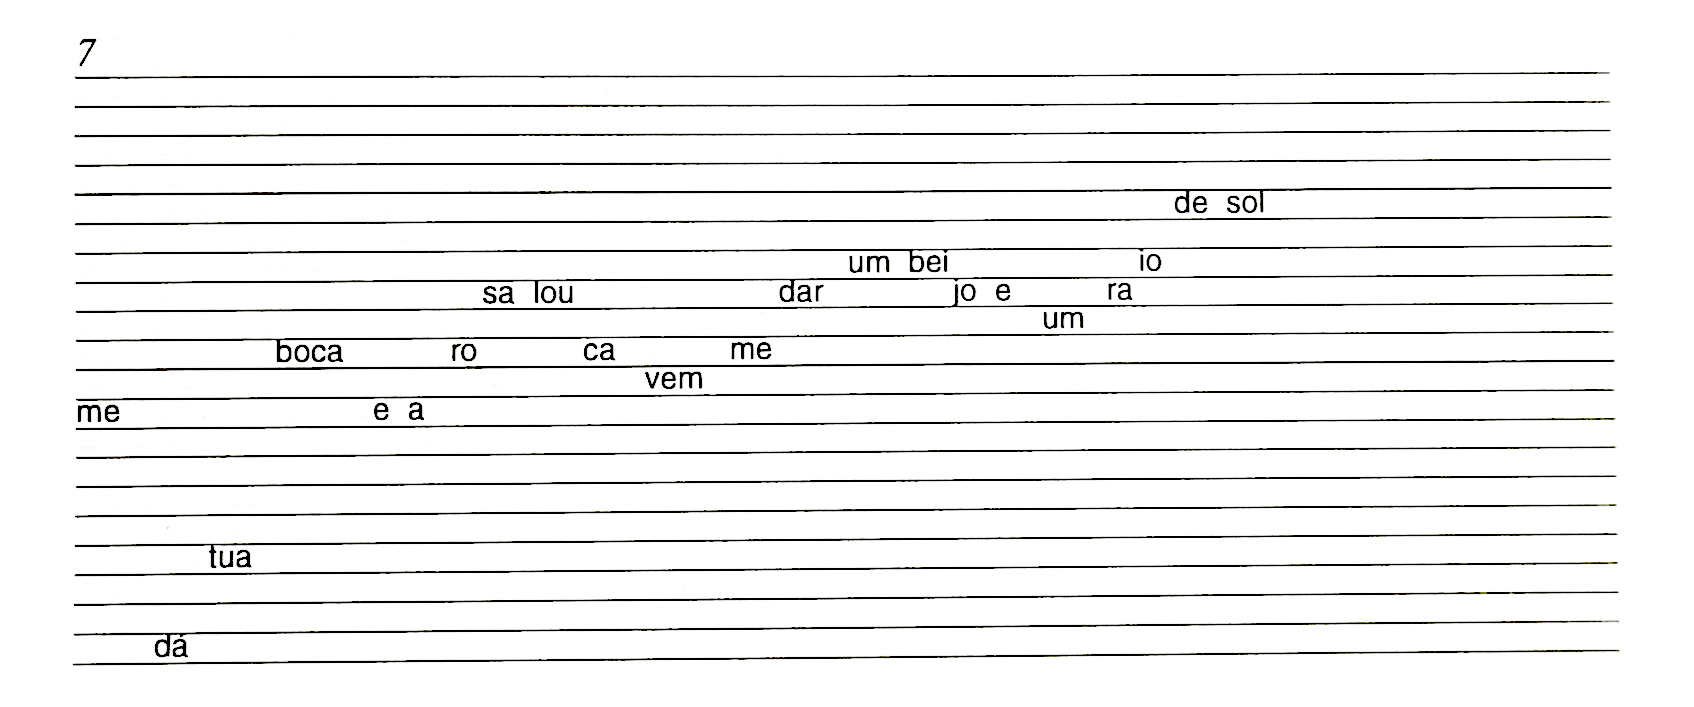
\includegraphics[width=\textwidth]{./imgs/figura19.jpg}

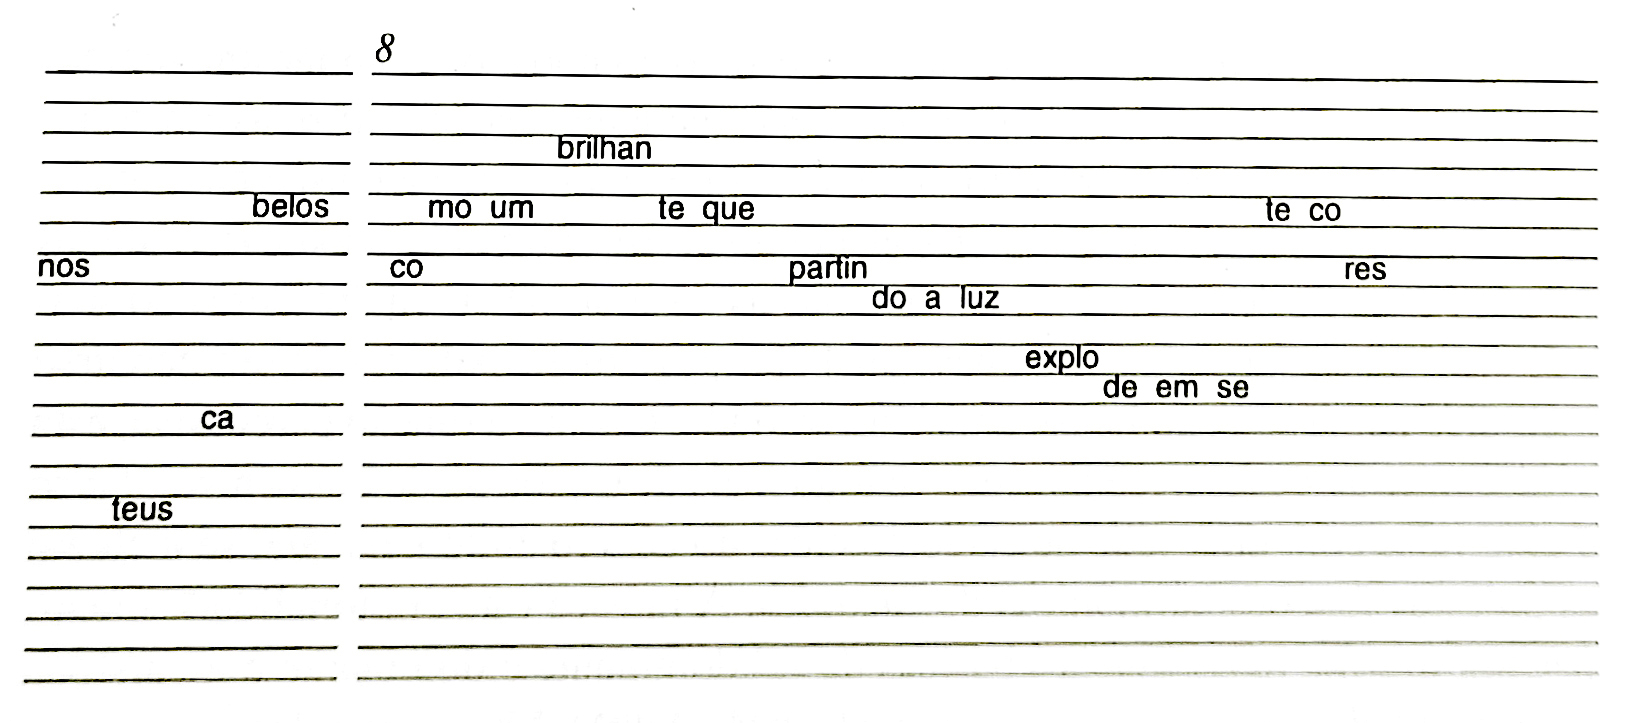
\includegraphics[width=\textwidth]{./imgs/figura20.jpg}
\end{figure}

\begin{figure}[H]
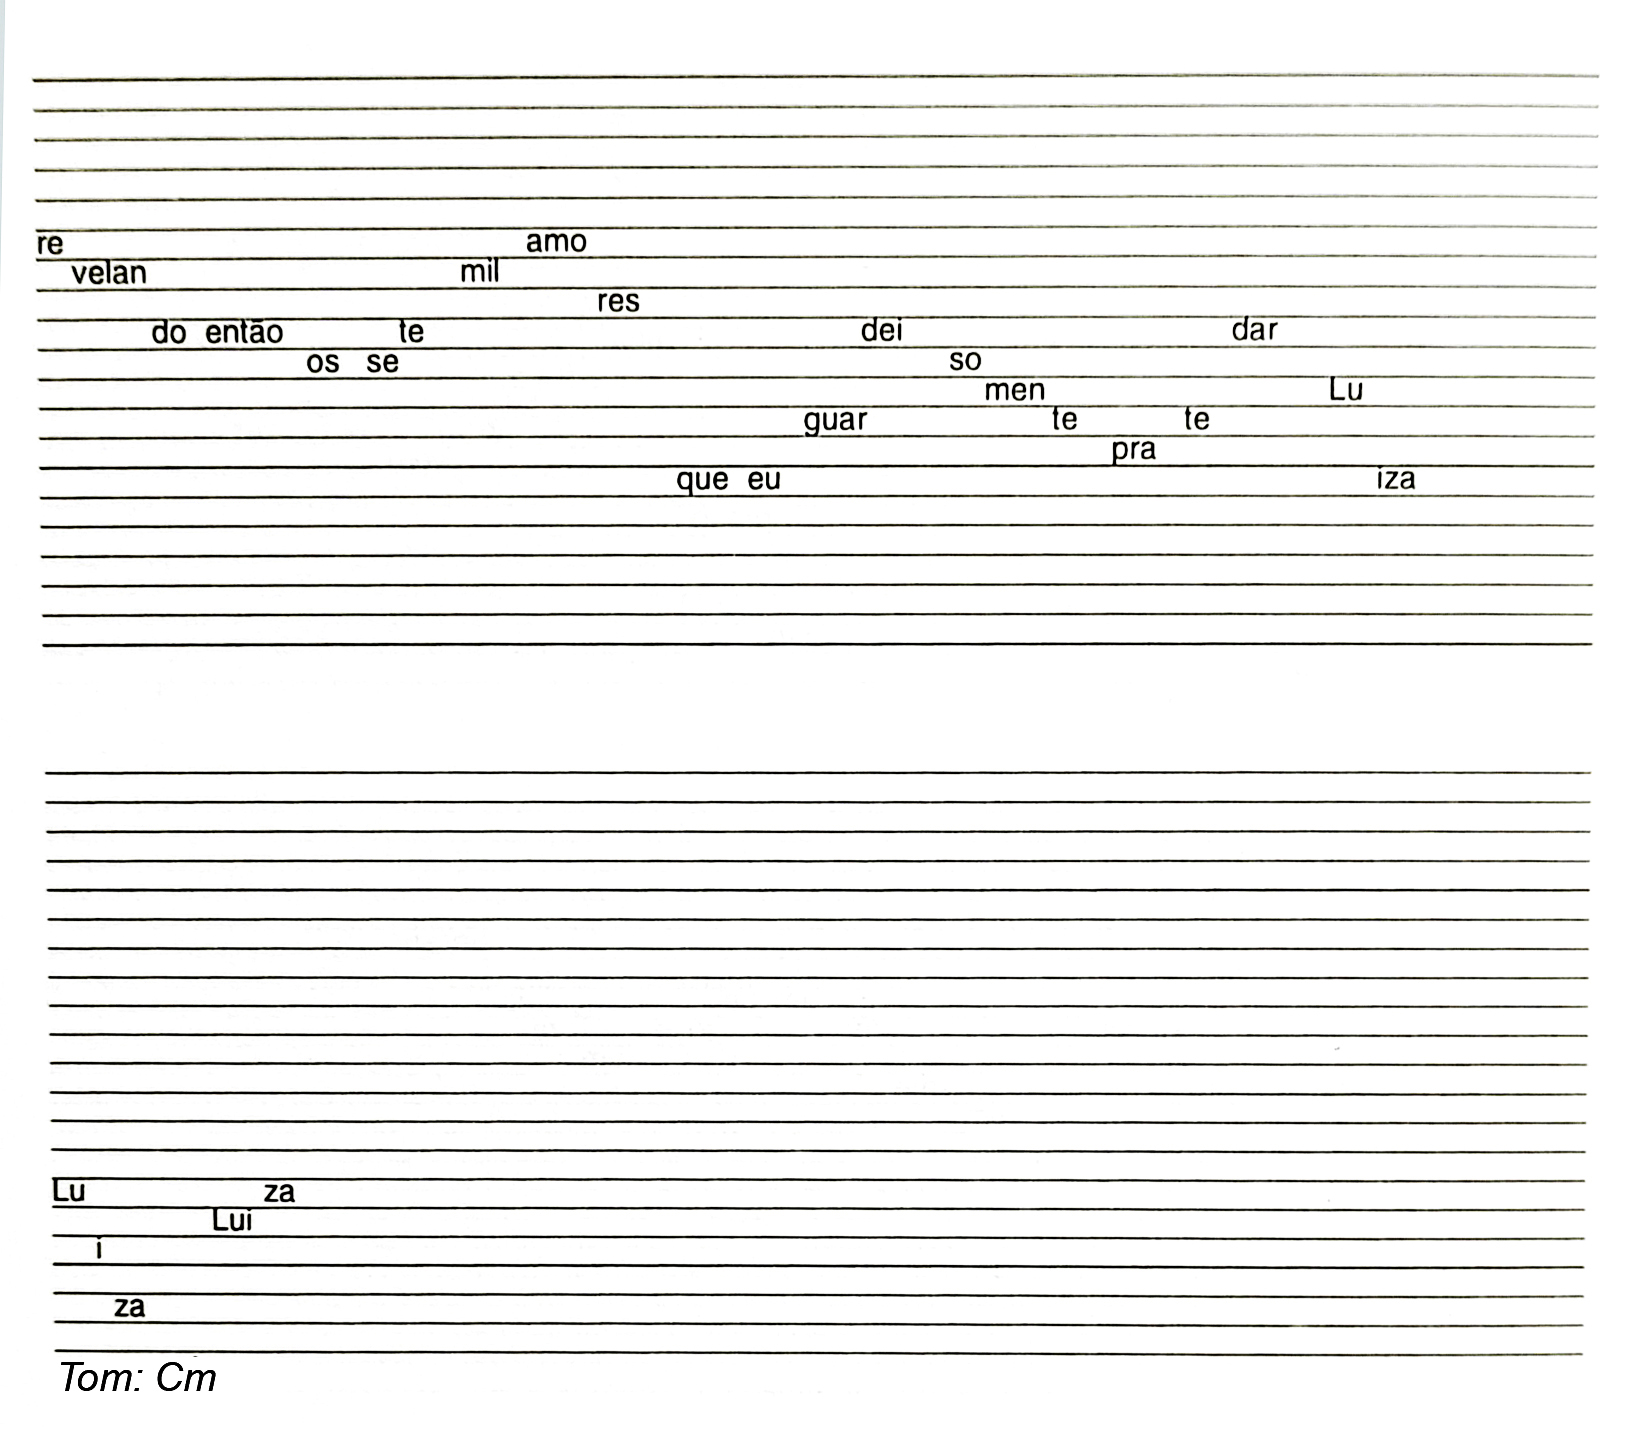
\includegraphics[width=\textwidth]{./imgs/figura21.jpg}
\end{figure}

``Luiza'' retrata uma outra faceta da dicção do compositor e, ao mesmo
tempo, revela um caráter cíclico na evolução da linguagem da canção.
Assim como outras composições do próprio Jobim, ela recupera
integralmente a tensão passional.

Embora conserve a marca dissonante no decorrer de toda a sua harmonia,
as funções dos acordes alterados não são mais as mesmas. De
modalizadores do sentido e condensadores da tensão passional eles passam
a auxiliares de um percurso melódico por si só complexo e altamente
variado. Quanto à função percussiva, esta evidentemente desaparece pois
não se trata mais de samba ou de bossa nova. ``Luiza'' é uma valsa com uma
série de características do gênero antigo, na qual se incluem as
próprias funções harmônicas dos acordes. A música está em tonalidade
menor (Cm), transita pelas funções básicas de subdominante e dominante
e incursiona por tonalidades relativas vizinhas como AbM e EbM. Mas os
acordes são tão dissonantes que temos a impressão de que a qualquer
momento o centro tonal pode ser abandonado definitivamente.

Tudo ocorre como se fosse a recuperação das melodias expansivas do
período pré-bossa nova, num contexto harmônico pós-bossa nova. Ao
ouvirmos, temos a impressão de uma fisionomia melódica conhecida, mas
com vários pontos de desengate que são ultrapassados mais pela força de
continuidade melódica do que pela solução harmônica. Em outras palavras,
o acorde não aponta a direção para melodia, engatando-a num encadeamento
harmônico, como era de praxe na bossa nova. Ele persegue seu curso
oferecendo, ao mesmo tempo, uma base e uma via de escape.

Mas, sem dúvida, o sentido volta a ser conduzido pelo contorno, e a
própria relação com a paixão reabilita seu vínculo existencial.

No texto, a disjunção amorosa é manifestada por um profundo sentimento
de falta e uma intensa necessidade e desejo de aproximação:

\begin{verse}
\small{Vem cá, Luiza, me dá sua mão\\
Me dá tua boca\ldots vem me dar um beijo\\
(\ldots) sete mil amores\\
Que eu ganhei somente\\
Pra te dar, Luiza}
\end{verse}

Para retratar esse estado de paixão, o percurso melódico é articulado
por dois componentes básicos: 

\begin{figure}[H]
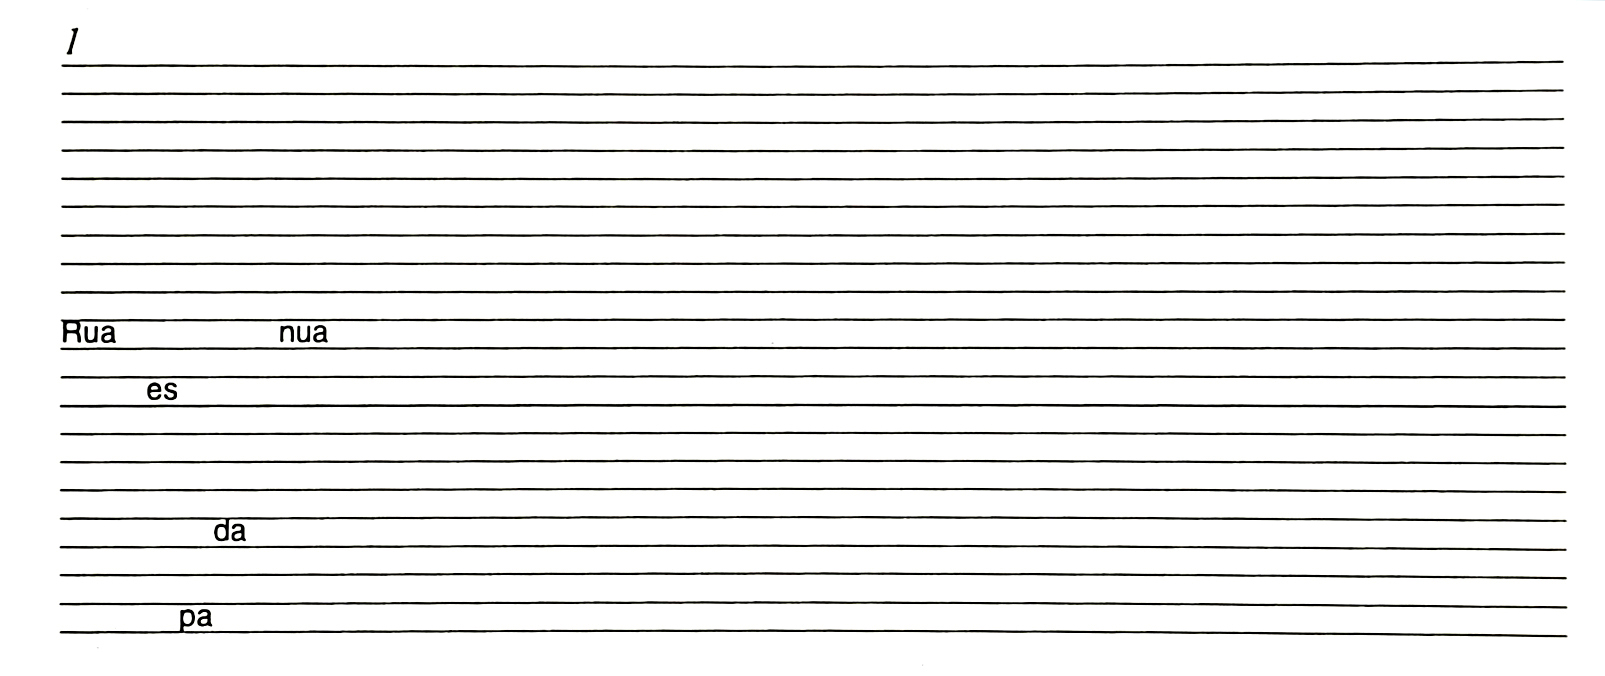
\includegraphics[width=\textwidth]{./imgs/figura22.jpg}
\end{figure}

\begin{enumerate}
\item Um módulo descontínuo delimitado por
pausas, com perfil em \textsc{v} e descrevendo saltos intervalares.

\item Uma sequência engrenada por graus conjuntos que, às vezes, se
dilatam em intervalos maiores, mas sempre em progressão contínua, sem
interrupções, até esbarrar em novo módulo.
\end{enumerate}

\begin{figure}[H]
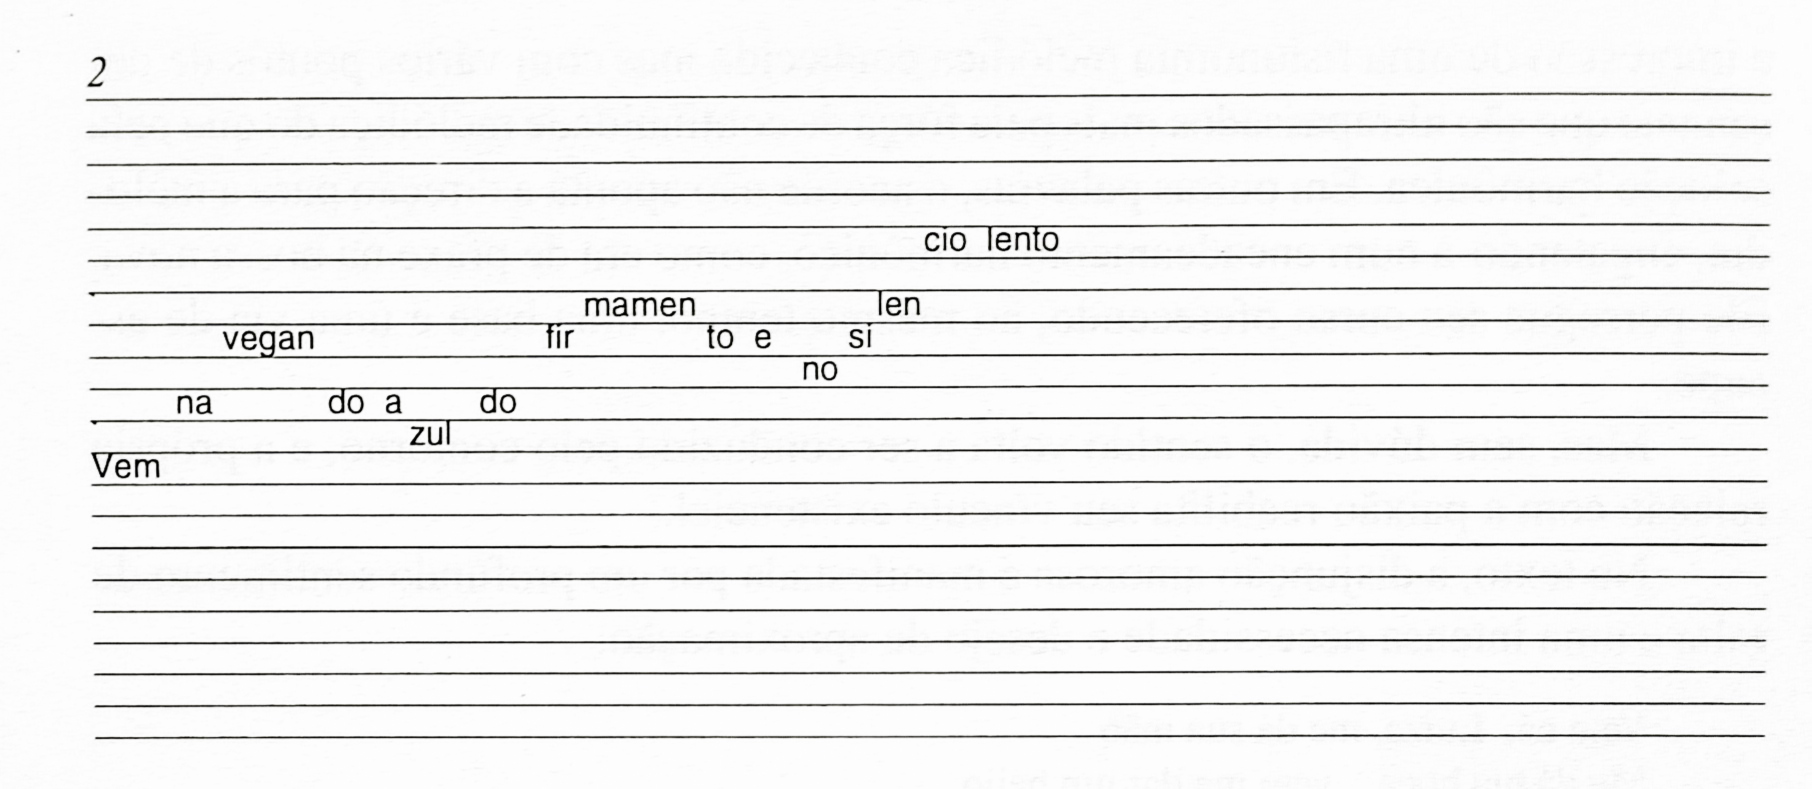
\includegraphics[width=\textwidth]{./imgs/figura23.jpg}
\end{figure}

Com os módulos, Jobim assegura a concentração sobre o \textit{ser} numa
permanente tensão flutuante. Os motivos formados com a amplos
intervalos, tonemas ascendentes e pausa final denotam um esforço
constante para se atingir a nota mais aguda pois não há gradação. A
emissão deve alcançar diretamente a frequência a partir de um impulso
sobre as notas graves. Durante toda a canção, esses módulos funcionam
como impulsos que mantém a tensão viva mas estável.

Com as sequências, o compositor realmente movimenta o estado passional
fazendo oscilar a margem de tensão investida.

Tudo ocorre como se os módulos representassem os estados de paixão
cristalizados em compasso de espera, e as sequências, as transformações
desses estados em termos de maior ou menor intensificação.

Nos dois primeiros segmentos temos uma espécie de projeto do que
prevalecerá por toda a canção: \textit{módulo--sequência--módulo--sequência}.

\begin{figure}[H]
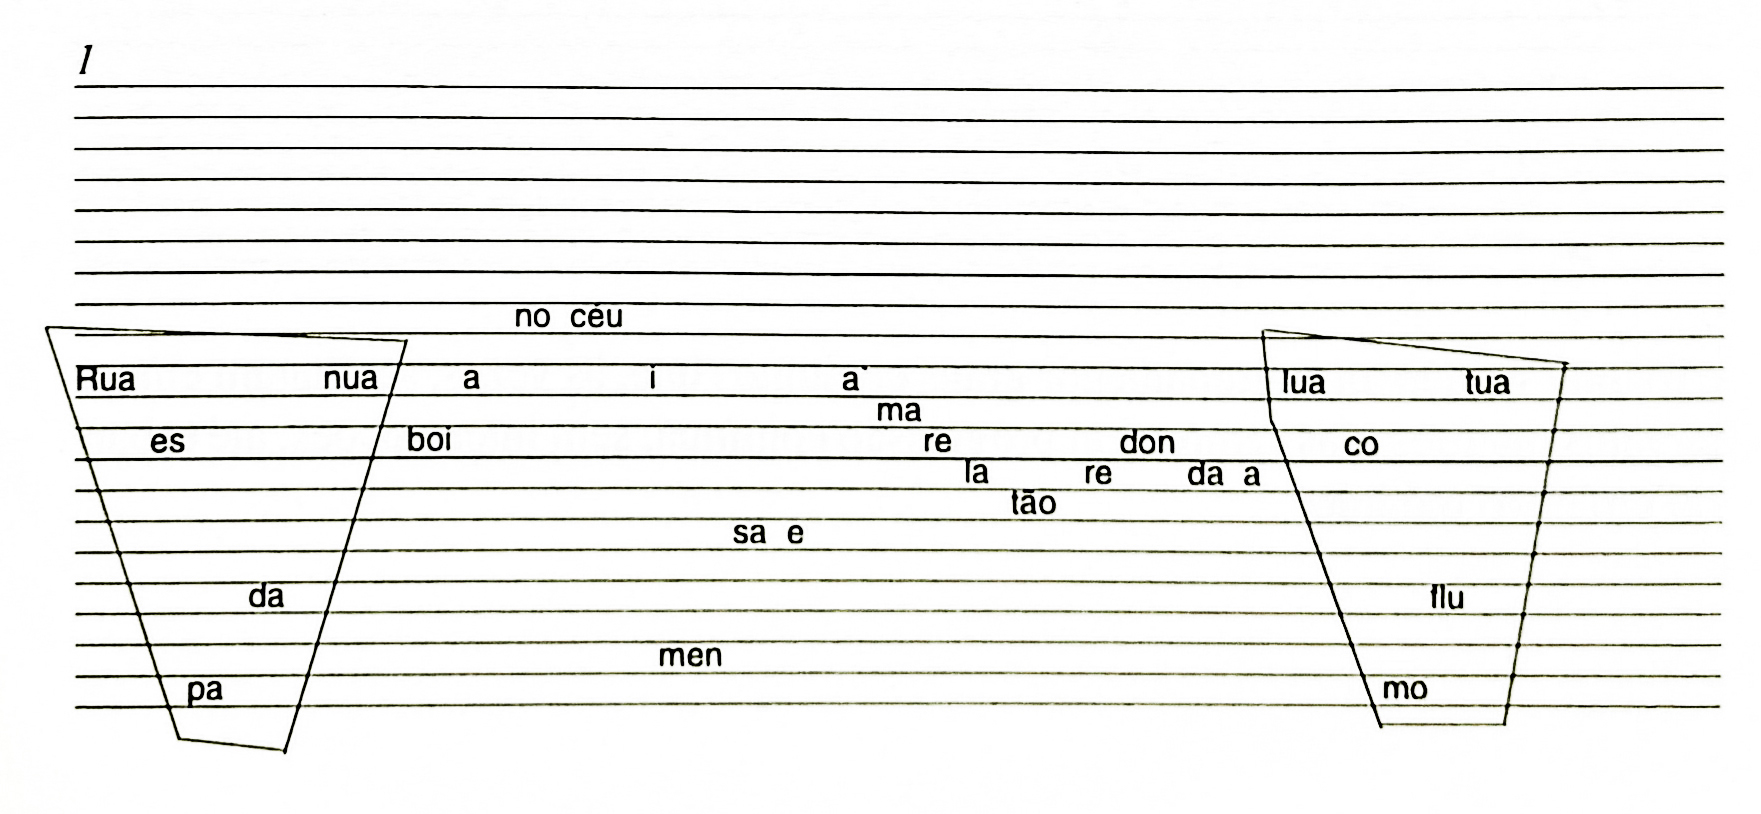
\includegraphics[width=\textwidth]{./imgs/figura24.jpg}

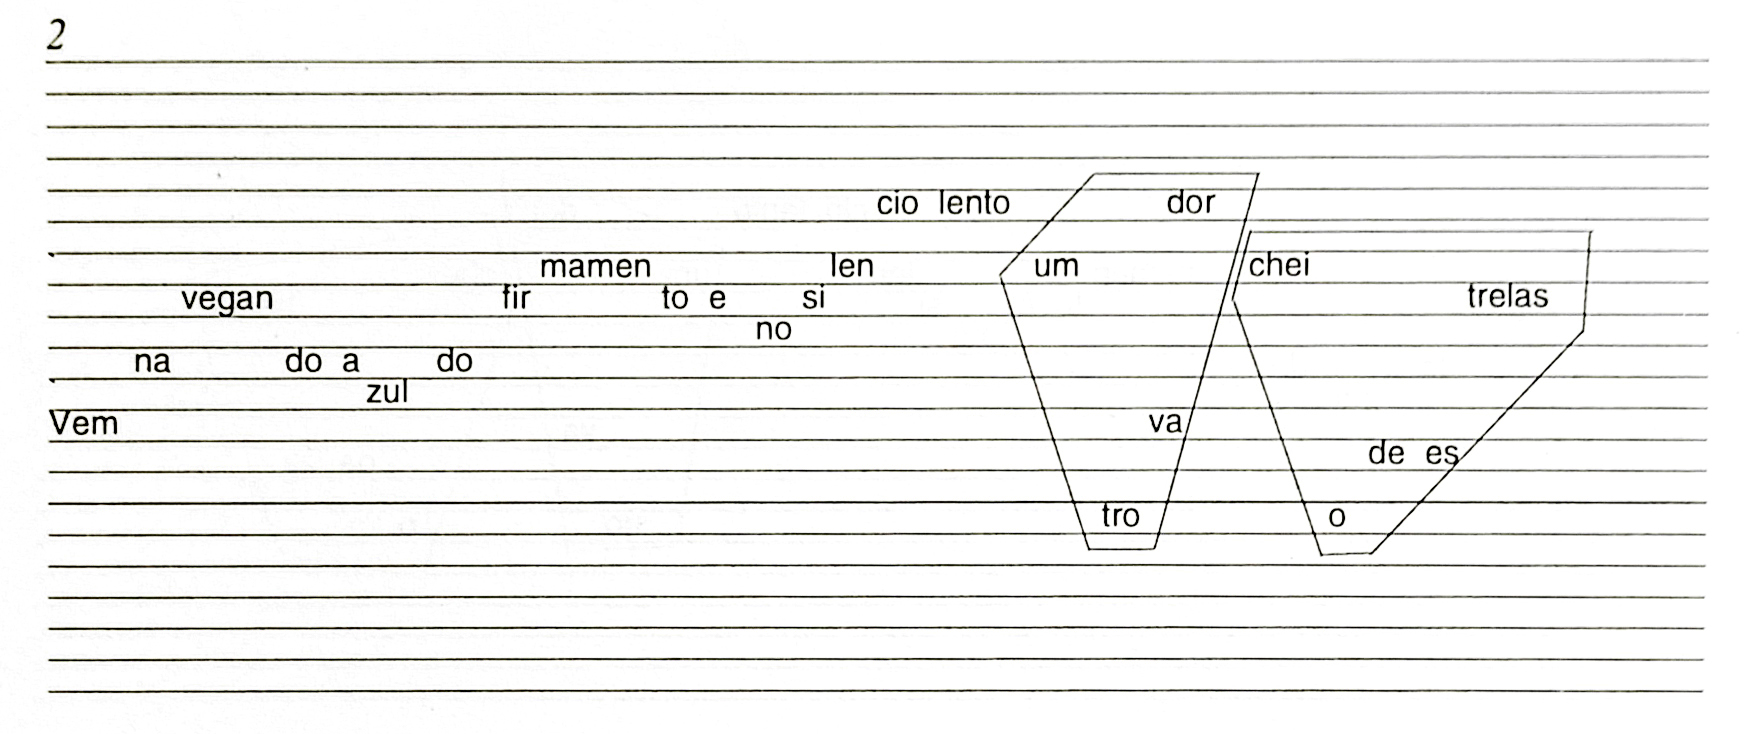
\includegraphics[width=\textwidth]{./imgs/figura25.jpg}
\end{figure}

Convém observar que, logo na primeira sequência, surge um fragmento de
memória melódica do módulo, mas já num contexto coordenado com o
movimento sequencial.

\begin{figure}[H]
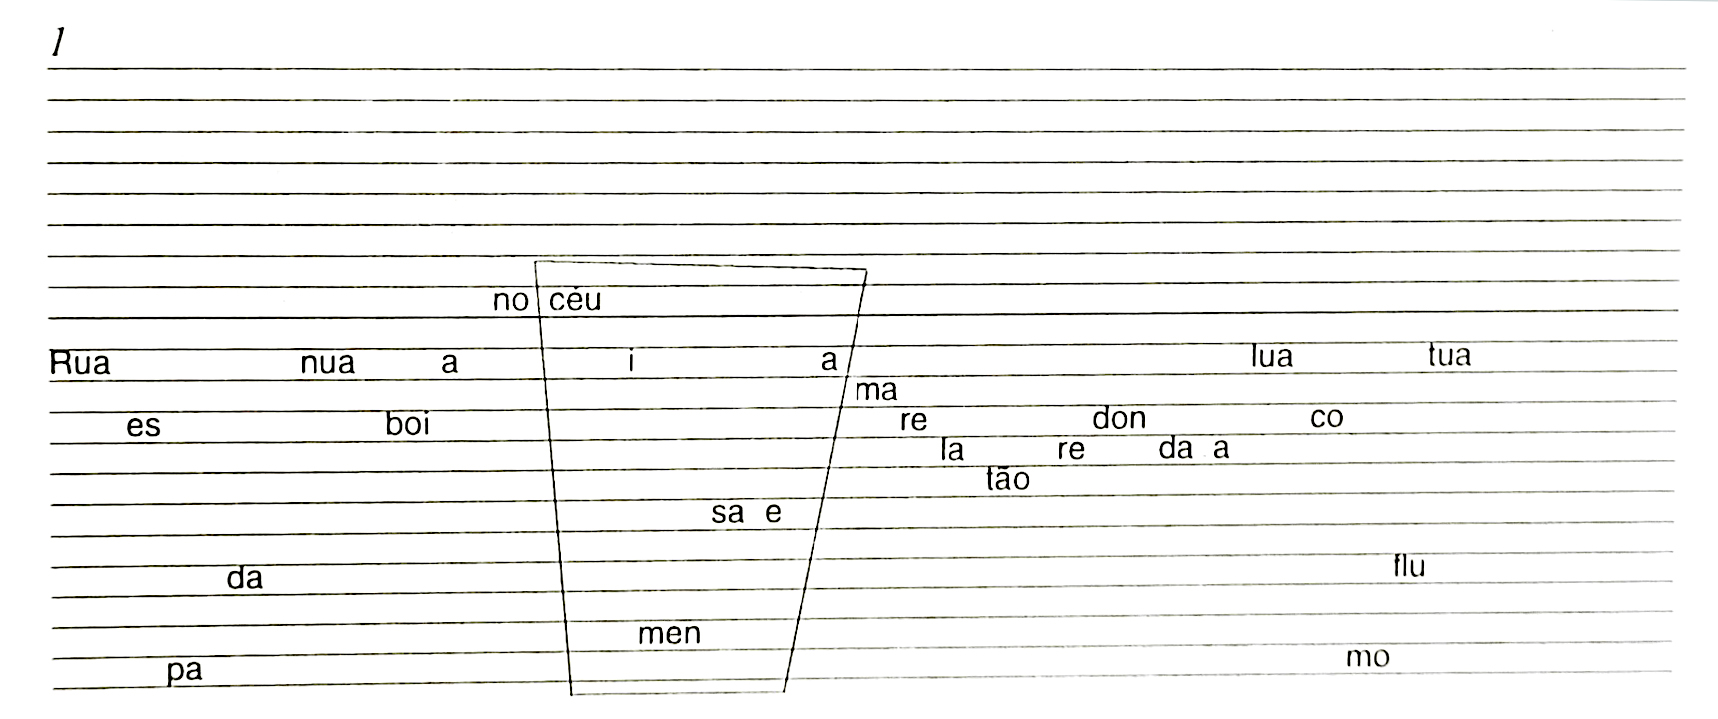
\includegraphics[width=\textwidth]{./imgs/figura26.jpg}
\end{figure}

Apesar de o desenho manter a semelhança, não há pausas isolando o motivo
e nem um tratamento especial em termos de duração. Suas sílabas são
pronunciadas com a mesma dinâmica das demais.

Este projeto melódico inicial está em sintonia com a extensa metáfora
introdutória que antecede a narrativa propriamente dita. Assim, ao se
deslanchar, no segundo segmento, a sequência engrenada descreve o
navegar da \textit{lua} em pleno \textit{firmamento} até ancorar no \textit{trovador
cheio de estrelas} com dois módulos anunciando o novo estado:

\begin{figure}[H]
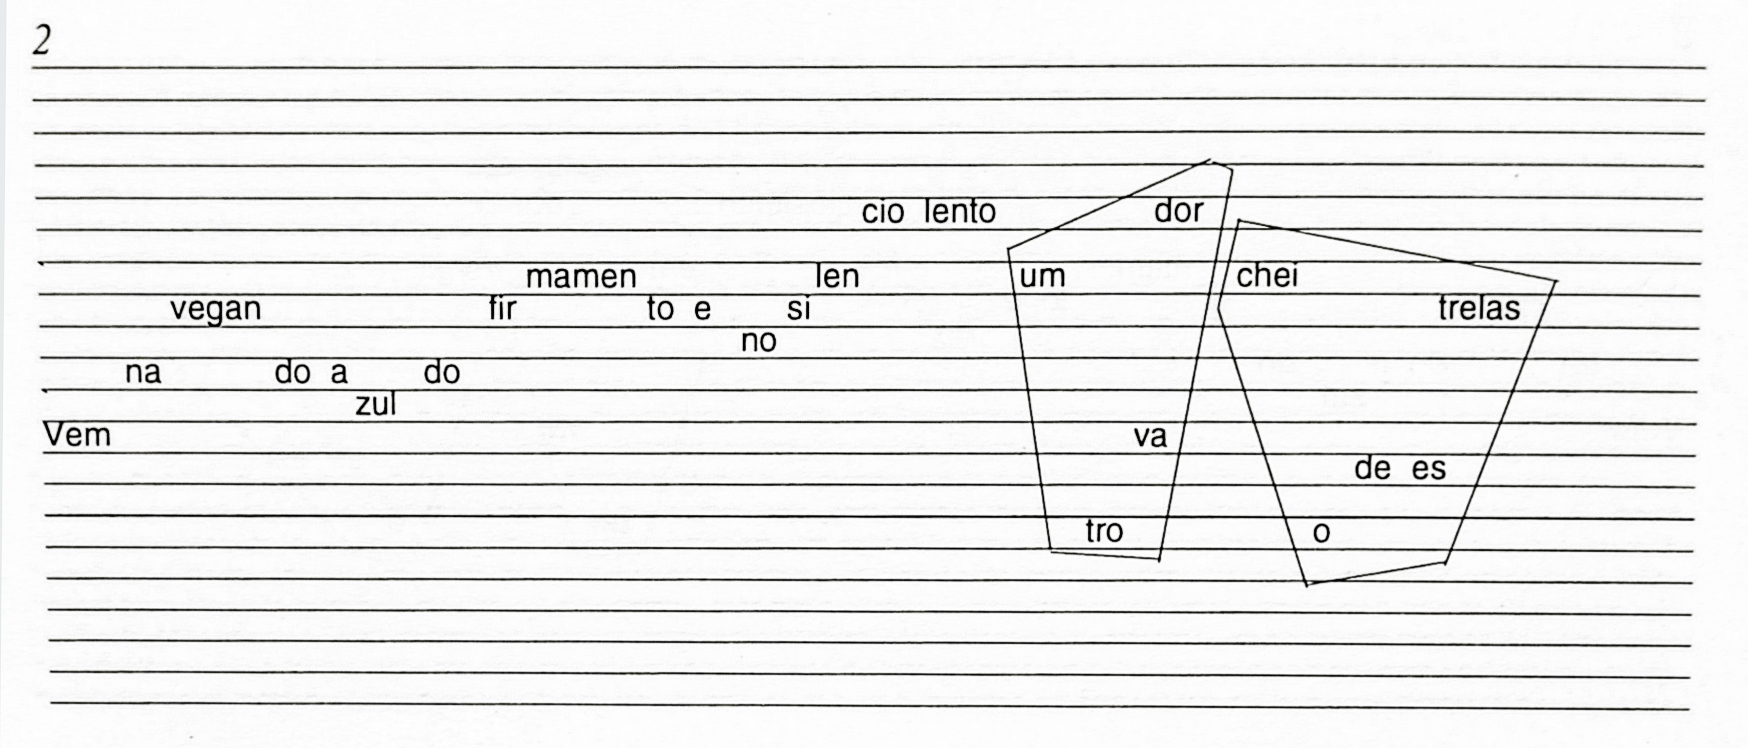
\includegraphics[width=\textwidth]{./imgs/figura27.jpg}
\end{figure}

Despontando a narrativa, no terceiro segmento, configura-se o núcleo da
tensão passional, com a identificação nominal do alvo do desejo do
enunciador --- \textit{Luiza} --- e com sua malograda tentativa de sustentar a
separação:

\begin{verse}
\small{Escuta agora a canção que eu fiz\\
Pra te esquecer, Luiza}
\end{verse}

O drama é registrado pela precipitação quase descontrolada da sequência
em direção ao ápice do agudo para, de lá, enunciar, pela primeira vez, o
nome da amada. A própria tonalidade menor se abre em \textsc{c7m}\,(9).

\begin{figure}[H]
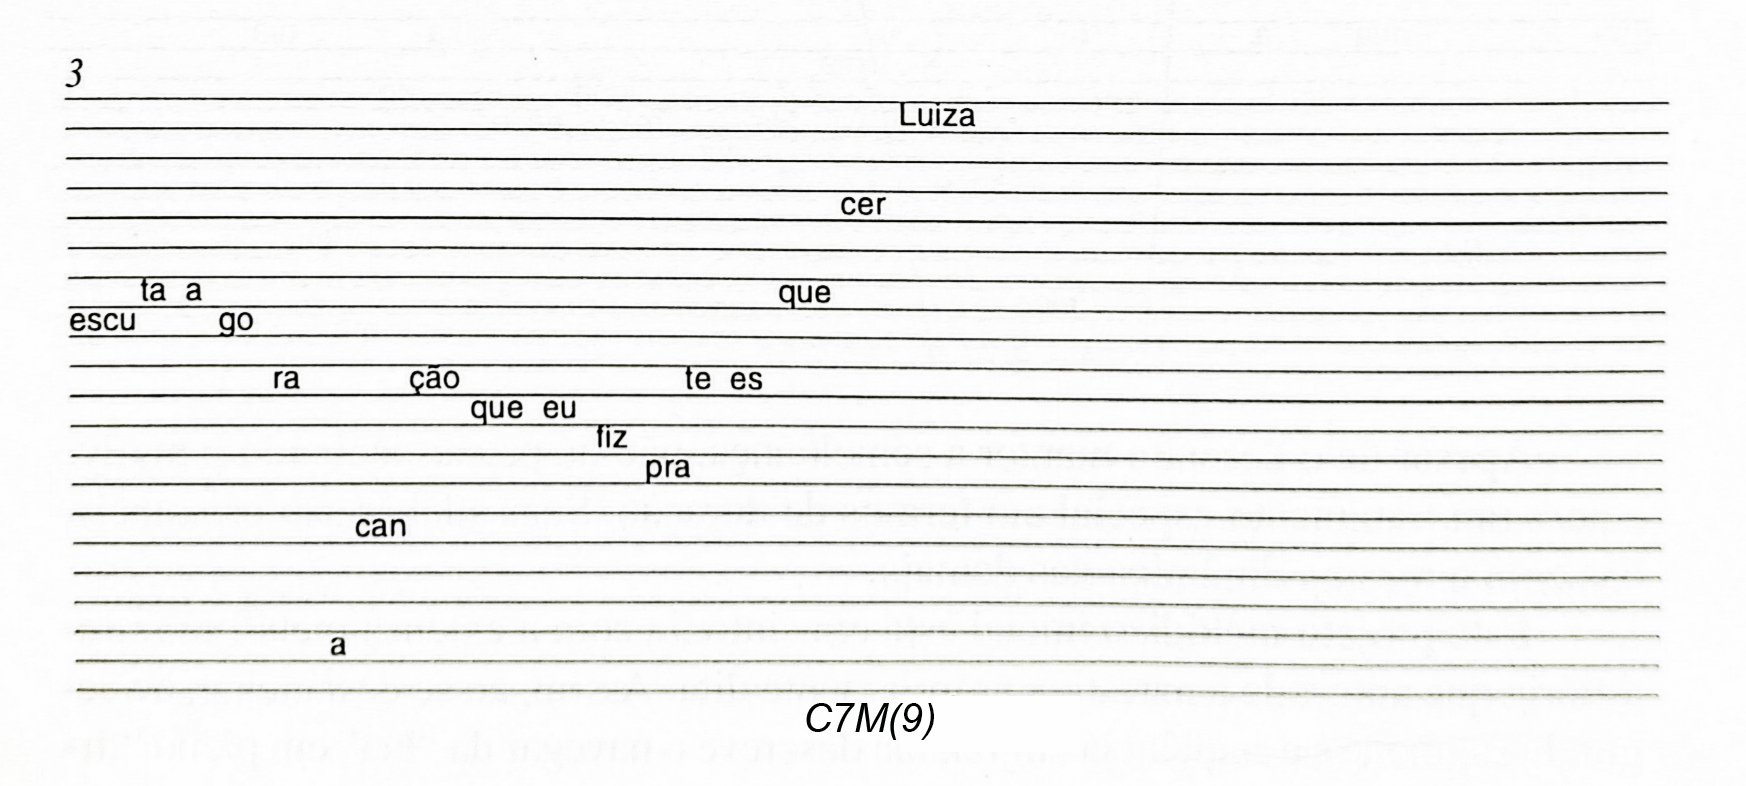
\includegraphics[width=\textwidth]{./imgs/figura28.jpg}
\end{figure}

Deste ponto máximo, atingido pela única vez em toda a canção, a melodia
escorre em distensão, mas, imediatamente, recobra o agudo, só que desta
feita sob a forma estável dos módulos. E numa sucessão desses, o
enunciador revela seu estado de \textit{amador}, \textit{apaixonado} e
\textit{aprendiz}.

\begin{figure}[H]
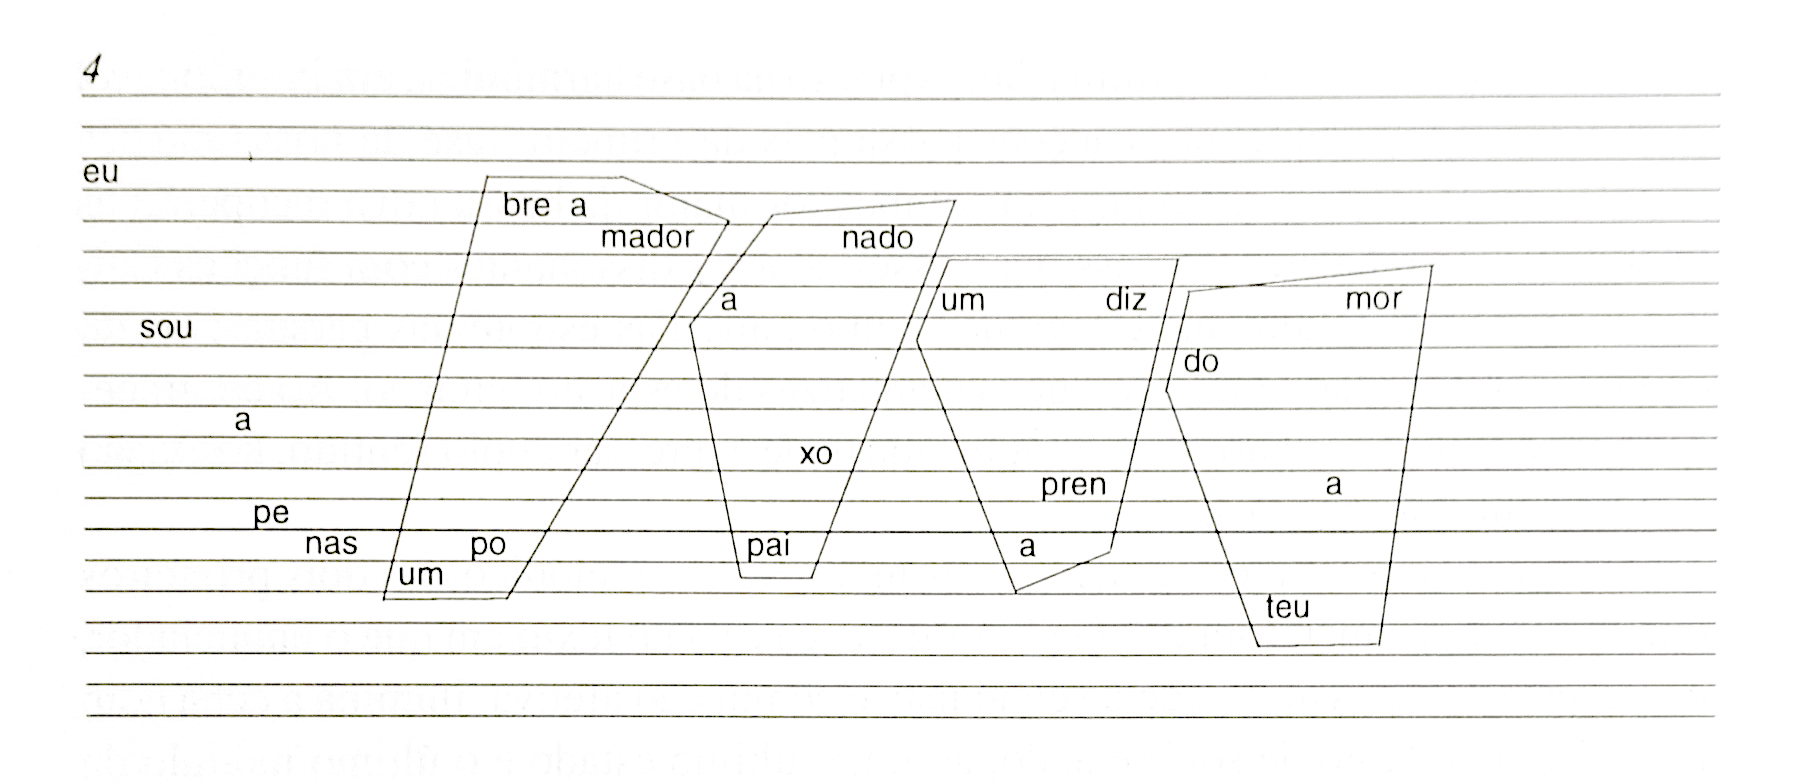
\includegraphics[width=\textwidth]{./imgs/figura29.jpg}
\end{figure}

Outro fator desponta no quinto segmento com a figura de um apelo à
sensibilidade da amada, numa sequência melódica que, novamente, busca a
tensão das alturas\ldots{} e chega a lugar nenhum.

\begin{figure}[H]
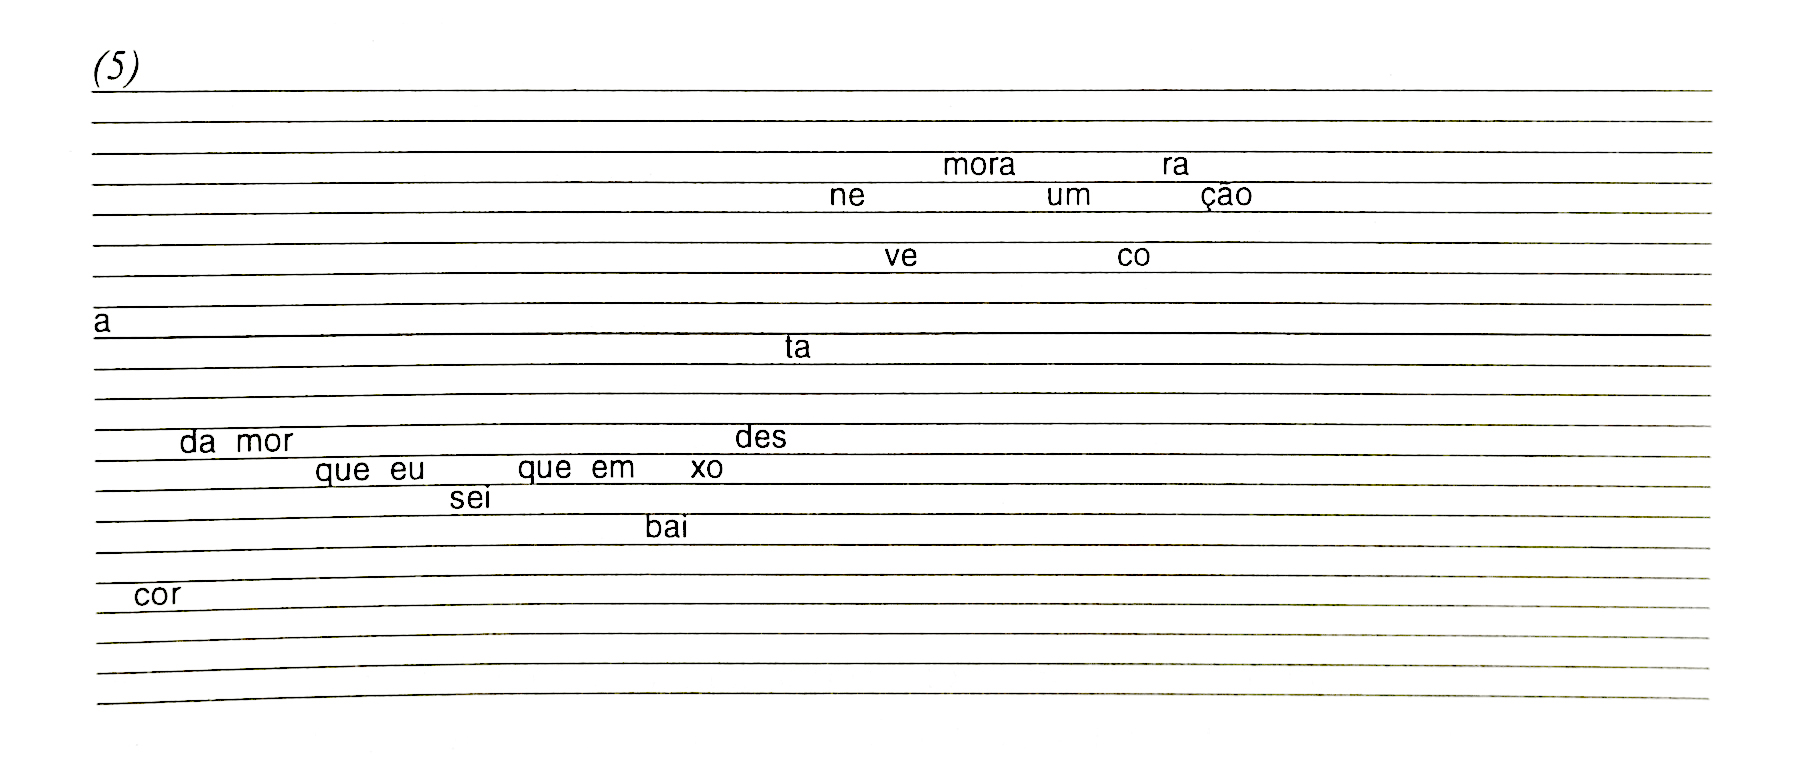
\includegraphics[width=\textwidth]{./imgs/figura30.jpg}
\end{figure}

Embora a melodia seja interrompida por uma pausa expressiva, após o
verbo \textit{mora}, para que \textit{um coração} soe como desenlace, do ponto de
vista harmônico o acorde não convence. Ou convence como indeterminação.
Trata-se de uma dominante individual (Db7) completamente deslocada de
contexto, difícil de analisar mesmo enquanto dominante. Se pensarmos
ainda em sua possível função conclusiva, então não há nada mais vago.
Como acorde de passagem, o seu papel fica um pouco mais claro: o baixo
desce cromaticamente de D (Dm7\,(9)), passa por esse Db (Db7) e atinge
C (Cm7) no segmento seguinte, já como acorde inicial (incoativo) e não
terminal. Esse parece o caminho mais plausível da progressão harmônica,
mas o fato é que ele conclui a frase com a mesma indefinição estampada
na letra. Nem o texto nem a melodia demonstram convicção na afirmativa
do enunciador.

Esse recurso de indeterminação, expresso na base harmônica, era
impraticável ou menos inconcebível nas canções passionais da primeira
fase de nossa música popular. Hoje, depois que o próprio compositor
maior da bossa nova recuperou as melodias de arrebatamento passional,
esses acordes dissonantes com funções fluidas já aparecem totalmente
integrados como parte das estratégias persuasivas do enunciador. Eles
facilitam a tradução de matizes do espírito humano. Ao contracenar com a
melodia, a harmonia enriquecida pode expressar duplo sentido, hesitação
e outras nuanças que tais.

O sexto e o sétimo segmentos repetem o trajeto melódico dos dois
primeiros que carreiam a metáfora da \textit{lua}. A diferença está no texto
em que o enunciador, considerando a possibilidade de conquistas e
conjunção afetiva, ilumina a cena com a metáfora do \textit{raio de sol}
selando, assim, o último estado e o último módulo da canção, no final do
segmento \textsc{vii}.

\begin{figure}[H]
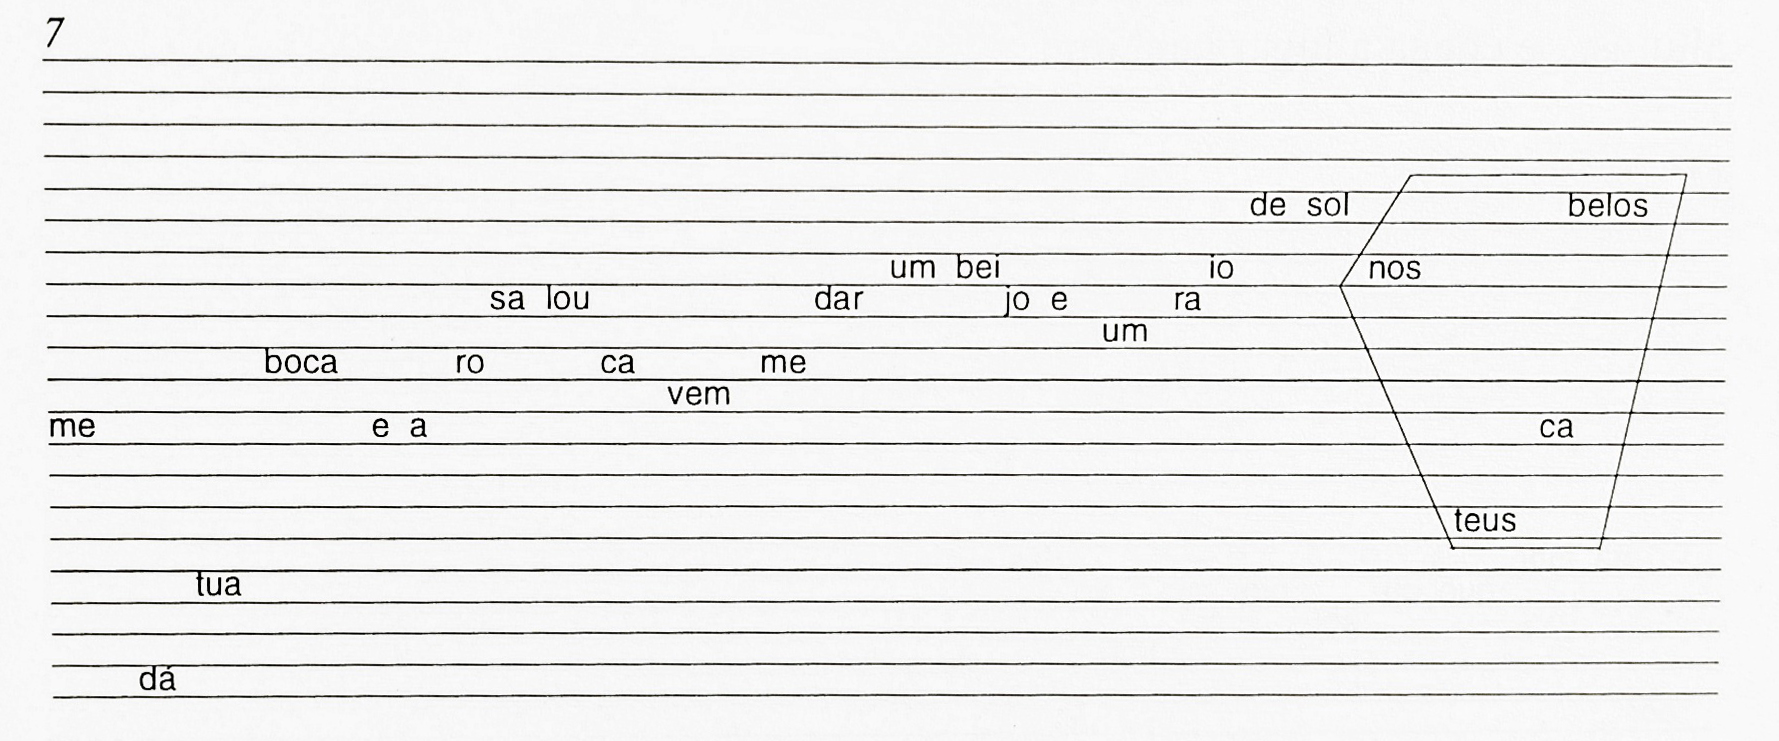
\includegraphics[width=\textwidth]{./imgs/figura31.jpg}
\end{figure}

A partir daí, deflagra-se a derradeira sequência melódica engrenada, com
um sentido conclusivo mas resvalando, em todo o percurso, na resistência
aflita da tentação passional. A imagem do \textit{brilhante} no ponto mais
agudo da sequência reluz nas elevações de \textit{sete cores} e de \textit{sete mil
amores} para depois a melodia se desativar num \textit{rallentando} já
impregnado de modalidade do \textit{ser}. Resta, por fim, o estado de amor e o
seu nome: \textit{Luiza}.

\begin{figure}[H]
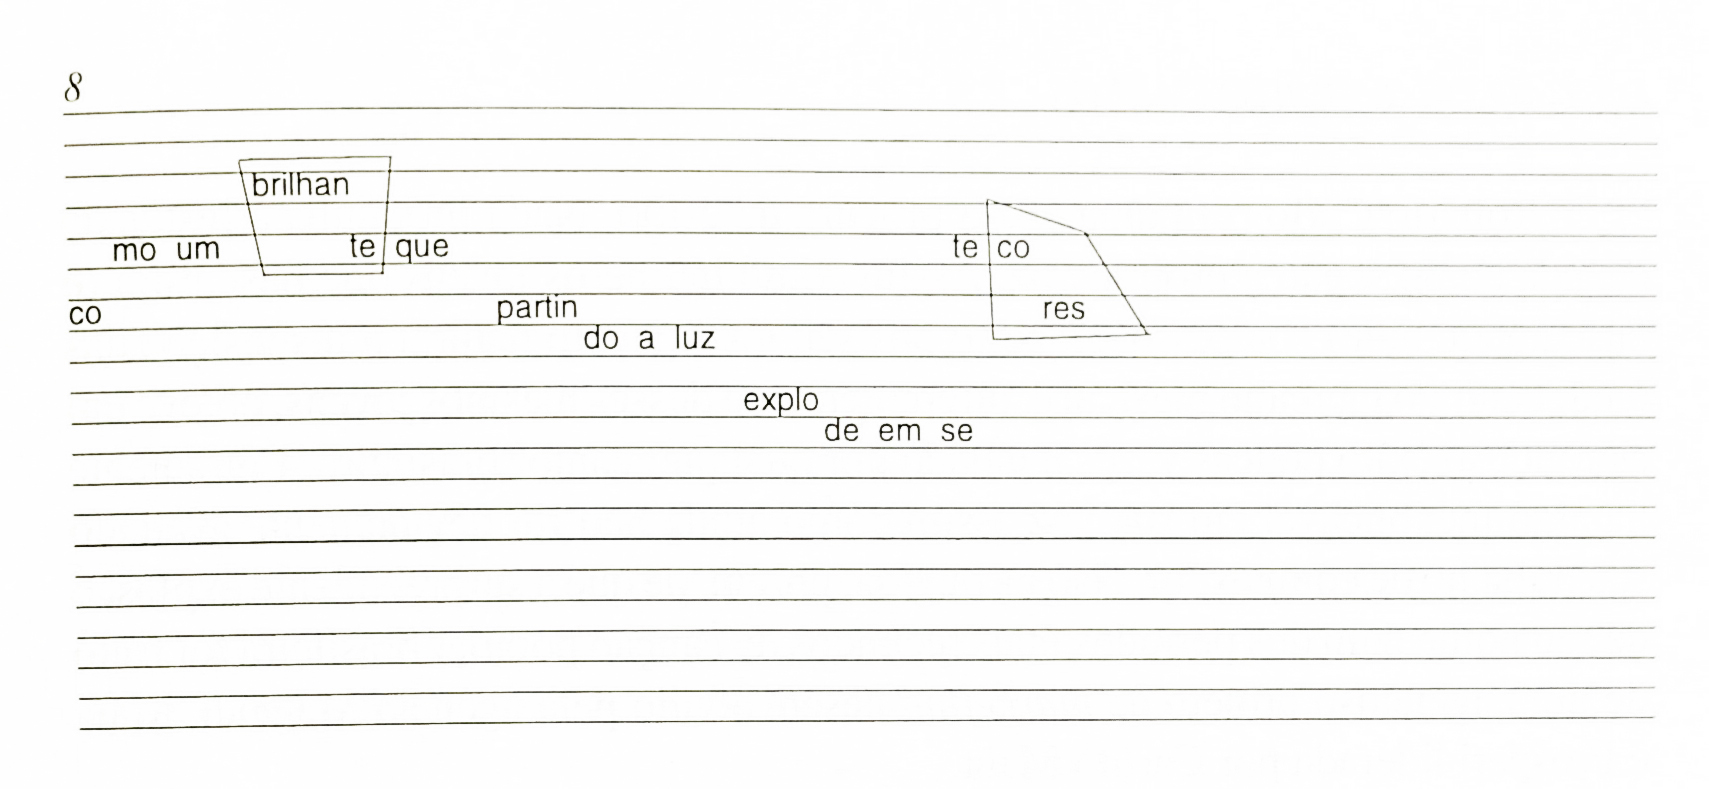
\includegraphics[width=\textwidth]{./imgs/figura32.jpg}

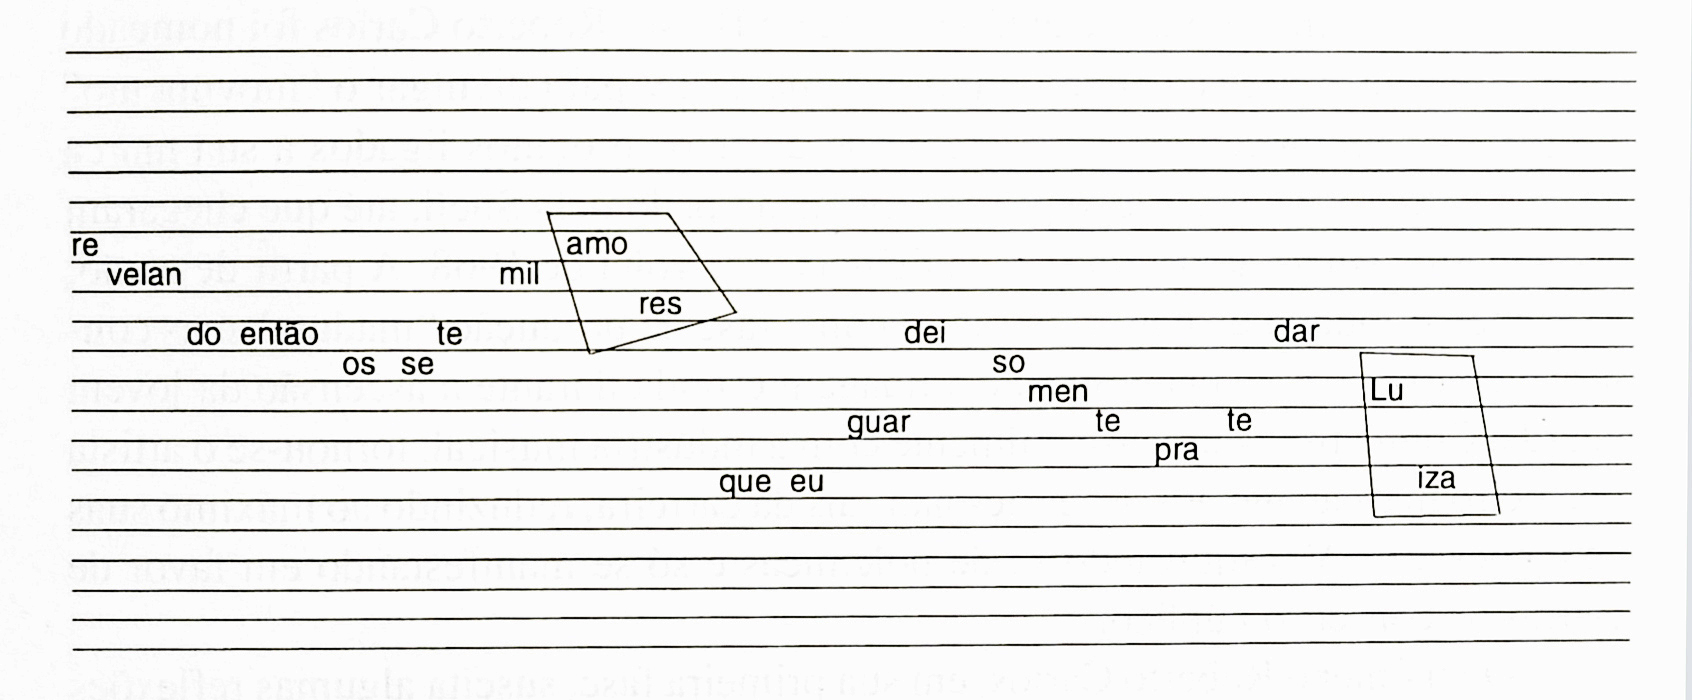
\includegraphics[width=\textwidth]{./imgs/figura33.jpg}

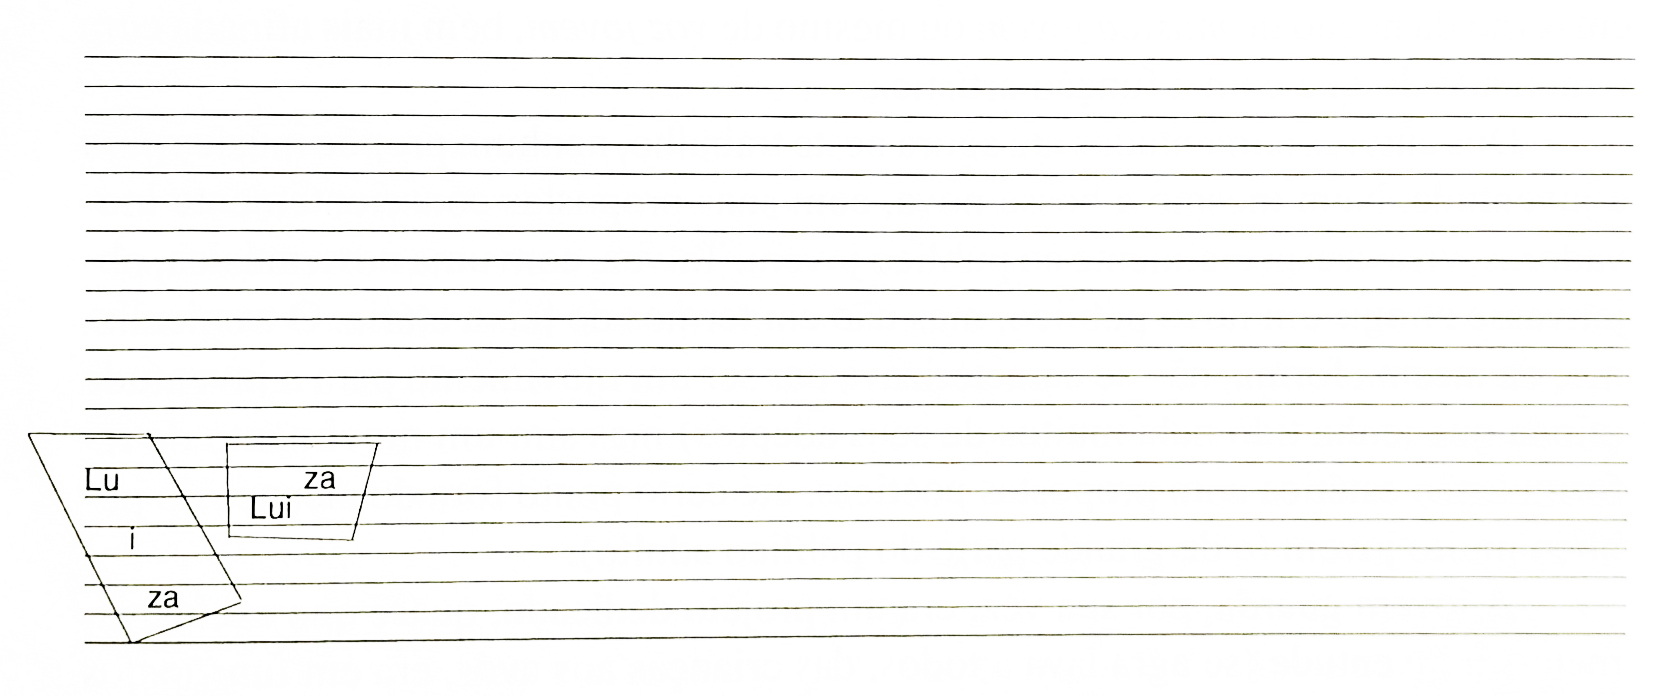
\includegraphics[width=\textwidth]{./imgs/figura34.jpg}
\end{figure}

\chapter{A transmutação do artista\footnote{Transcrição do capítulo ``A transmutação do artista'', presente em \textit{Todos entoam: ensaios, conversas e canções}, publicado pela Publifolha. O livro conta com 16 ensaios sobre a canção popular, e acompanha comentários e memórias da infância e adolescência de Luiz Tatit.}}


Itamar Assumpção pode ser compreendido como o artista que fez caber um
\textit{eu} imenso nos limites da canção. Dotado de um verdadeiro manancial
criativo, o compositor sempre precisou dizer, ou cantar, diversas frases
ao mesmo tempo, inserir numa simples cantiga numerosos acontecimentos
musicais e, mesmo assim, sua obra só se completava no disco integral,
pleno de retomadas, vinhetas e comentários de toda espécie. Mas nem o
disco lhe parecia suficiente. Seu ponto de partida era, no mínimo, uma
trilogia. Não deixava escapar uma experiência, uma observação, nem mesmo
uma brincadeira, sem convertê-las instantaneamente em letra, melodia e
arranjo instrumental, como se tivesse a missão de escrever a crônica de
toda uma vida e guardá-la num formato de obra que ele próprio criou.

Suas primeiras composições eram altamente comprometidas com o
Itamar-cantor. Assinalavam a presença de sua voz grave e até de seu
corpo esguio como condição indispensável para o entendimento mais
profundo daquilo que apresentava. Aos poucos essa forte personalidade
extramusical foi-se transformando em traços de estilo sonoro no interior
das composições, de modo que outros intérpretes puderam enfim se
apropriar da dicção de Beleléu e trazê-la ao mercado aberto de discos. A
pergunta essencial e o grande desafio para quem quiser começar a
refletir sobre o fenômeno Itamar Assumpção podem talvez se resumir na
seguinte formulação: como esse \textit{eu}, tão fecundo quanto
característico, acabou se alojando no cerne da canção popular brasileira
e se tornando marca de qualidade artística disputada por grandes
expoentes de nossa música?

\section{a enunciação do cancionista}

Todos sabem que dizer \textit{eu} num texto qualquer, oral ou escrito,
significa comprometer o enunciador com o conteúdo dito. Numa letra de
canção já contando com a inflexão melódica, dizer \textit{eu} é encarnar
alguém que expressa no exato momento em que canta. Afinal, emitir
conteúdos com modulações entoativas é a prática mais habitual de todo
ser humano. Baseados nisso, os intérpretes fazem de tudo para transmitir
aos ouvintes um envolvimento pessoal com aquilo que dizem na letra.

Claro que não preciso dizer \textit{eu} literalmente para me fazer sentir
como enunciador do texto. Quando digo \textit{você}, \textit{tu}, \textit{o senhor} ou
qualquer outro indício de que me dirijo a alguém --- imperativos,
demonstrativos, nome próprios etc.---, imediatamente me instalo como
\textit{eu}, já que ninguém pode dirigir ao outro sem estar presente. E
quando o texto é oral, ou cancional, conduzido por entoações ou
melodias, essa presença torna-se física, se não pela participação do
corpo do enunciador, como num show, no mínimo pela atuação da voz, como
num disco.

Assim, toda canção tende a ser a história do intérprete, a menos que
este lance mão de recursos para torná-la mais \textit{objetiva}. É o caso das
interpretações mais técnicas, em que o cantor prefere ostentar seus
dotes musicais a deixar transparecer suas ênfases entoativas. Mas o que
tem normalmente, é um jogo de oscilações entre formas subjetivas e
objetiva: de veicular a canção, de maneira que o ouvinte possa tanto se
encantar com a sinceridade do cantor quanto se divertir com sua ironia
ou crítica velada ao conteúdo da letra.

Itamar trouxe de sua vivência teatral de juventude um personagem que
sempre o acompanhou nas apresentações musicais, como uma espécie \textit{eu}
absoluto cuja história só poderia ser desvendada pelas canções. A cada
show e a cada novo disco, os ouvintes conheciam um pouco mais desse
mundo subjetivo, porém, davam-se conta de que este \textit{eu}
transformava-se em outros e tornava-se inesgotável.

\section{beleléu}

Em \textit{Beleléu}, o \textit{eu} do compositor e intérprete Itamar Assumpção ganhou
nome, sobrenome e pseudônimo: Benedito João dos Santos Silva Beleléu,
vulgo \textit{nego dito}. Mas ganhou também uma identidade musical que atravessou
toda a sua carreira de pouco mais de duas décadas: o rock de breque
(guitarra, baixo, bateria e a própria voz articulando frases
interrompidas), o diálogo com o backing vocal, os acontecimentos
musicais simultâneos e a força centralizadora dos refrões. À maneira de
\textit{Sgt. Pepper's}, o \textsc{lp} era inteiramente dedicado às peripécias de seus
artistas. Mas enquanto os músicos ingleses cantavam as carências
amorosas da famosíssima banda, Itamar contava as proezas e os fracassos
de seu \textit{perigosíssimo bando}. Se lá os meninos de Liverpool \textit{se
sentiam ligados a um sargento}, aqui, os instrumentistas marginalizados
se sentiam como isca de polícia, não querendo nada com milícias ou
qualquer corporação disciplinar. Se lá reinava a música branca, criada
pela família Lennon-McCartney, aqui prevalecia a \textit{nega música}
produzida pelo \textit{nego dito} que não transava parente. Talvez polos
diurno e noturno do mesmo talento.

O \textit{eu-Beleléu} contribuiu sem dúvida para uma associação direta
da sonoridade do disco com o seu protagonista. A negritude, a
marginalidade musical, a loucura descrita em muitas passagens das
letras, tudo isso convocava a figura magra e enigmática do autor que,
por sua vez, nada fazia para dissociar personagem do ser em carne e
osso. A complexidade rítmica dos arranjos denunciava as origens
africanas; a singularidade das soluções musicais, embora fosse
imediatamente reconhecida pelo público fiel, constituía uma \textit{barreira} a
mais para o seu ingresso na produção em série do mainstream; por fim, os
desatinos explícitos de Beleléu misturavam-se às idiossincrasias do
compositor, pouco ou nada afeito a concessões.

Mas, por incrível que pareça, havia também uma distância entre o
indivíduo Itamar e seu personagem assinalada pelas caricaturas vocais,
pelas tiradas humorísticas e pela ironia com a própria condição de
artista excluído. As locuções radiofônicas à moda dos programas
mundo-cão --- \textit{finalmente Beleléu e a banda Isca de polícia resolveram se
entregar}\ldots ---, as vinhetas e, sobretudo, as intervenções do vocal, que
saltavam do fundo para o primeiro plano, sempre exerceram funções
apreciativas maliciosas, desfazendo o elo imediato do intérprete com seu
conteúdo. Beleléu virava então um anti-herói de gibi, com atitudes
caricaturais risíveis, mas não totalmente impossíveis. Embora nesse caso
prevalecesse uma certa distância satírica, O criador nunca fez questão
de se afastar demais da criatura.

O eu-Beleléu ancorava-se nesse disco em pelo menos quatro refrões
inesquecíveis, todos eles retratando situações de fala nas quais o
personagem se definia não apenas pelo que era, mas igualmente pelo que
dizia a seu interlocutor. Em primeiro lugar, o famoso \textit{Benedito João
dos Santos Silva Beleléu /\,vulgo nego dito, nego dito cascavé}, de ``Nego
Dito'' já se configurava de saída \textbar{} como uma resposta em forma de
vinheta, que se estendia desta canção para outros momentos do disco.
Resposta a quem pudesse pôr em dúvida a identidade do novo personagem,
símile do artista recém-chegado, que convertia a exclusão em acolhimento
musical expresso no convite irresistível ao canto: o encaixe engenhoso
dos acentos melódicos nas sílabas de \textit{Benedito João dos Santos
Silva}\ldots levava o público a entoar em coro o refrão, encarnando de
algum modo o ponto de vista de Beleléu. E uma vez nesta perspectiva, não
era difícil assumir os demais estribilhos que apenas detalhavam a
personalidade do \textit{nego dito}, seja no âmbito do desvario, \textit{fico louco
faço cara de mau /\,falo o que me vem na cabeça} (``Fico louco''), seja nos
imperativos de intolerância, \textbar{} \textit{deixa de conversa mole, Luzia
/\,deixa de conversa mole}\ldots (``Luzia''), seja ainda nas poucas situações
românticas, \textit{não venha querendo você se espantar /\,não, não, não, não,
não}\ldots (``Nega música'').

\section{às próprias custas s.\,a.}

Os refrões de \textit{Beleléu} garantiram a cumplicidade necessária para que o
artista e seu público ingressassem na aventura explícita de \textit{Às próprias
custas}. Esse disco, gravado ao vivo em São Paulo, na sala Guiomar
Novaes, era um misto de vida de palco, diálogo com compositores de todos
os credos --- de Adoniran a Arrigo, passando por Geraldo Pereira, Macalé e
Getúlio Côrtes --- experimentação musical e barateamento de custo. Mais
uma vez, o \textsc{lp} era concebido como história única, um programa de rádio
cujo título, \textit{Mais lenha nesse inferno}, já definia o espírito do
aqui-agora vivido no palco. Sob um arranjo instrumental contundente,
repleto de \textit{ostinatos} e breques, as primeiras canções mal podiam ser
reconhecidas como obras de seus autores originais, dada a nova função
que adquiriam no longo pronunciamento do cantor. Itamar continuava
dando respostas ao samba consagrado, à música pop, ao experimentalismo
erudito e aos algozes do dia a dia. O \textit{eu} intenso do artista estava
sempre ameaçado por brigas, denúncias, preconceitos e até por
Frankstein!

\textit{Às próprias custas \textsc{s.\,a.}} era o disco do réu. Do modo de produção --- as
desvantagens técnicas de um \textsc{lp} gravado ao vivo naqueles idos dos anos
1980 eram flagrantes --- ao repertório repleto de situações de cerco,
bloqueio e condenação, além da rendição redigida e assinada pelo autor
na contracapa, tudo fazia do espetáculo uma sessão de julgamento em que
o réu só tinha a seu favor a cumplicidade do público. No mais, a culpa
por ter nascido com suas características e condições de vida: \textit{Peço
perdão pela minha ignorância /\,Eu venho assim desde a minha infância}
(``Peço perdão''). Seu único libelo contra todas as acusações era a força
das próprias canções. ``Batuque'', por exemplo, era a expansão comovente de
seu enfoque pessoal à história da raça negra. A melodia descendente, que
desemboca no batuque propriamente dito (\textit{Deu bandeira /\,dançou na
primeira /\,dançou capoeira /\,dançou de bobeira}\ldots), garantia à
composição um espírito de rito em homenagem ao sofrimento do povo
tradicionalmente escravizado. Um belo tributo ao réu coletivo. ``Que
barato'' e ``Denúncia dos Santos Silva Beleléu'' particularizavam a cena do
réu indefensável entoando suas justificativas satíricas em meio às
frases frias, cortantes e cortadas das guitarras algozes.

\section{sampa midnight: isso não vai ficar assim}

O programa radiofônico, que alegorizava a conversa direta do \textit{nego dito}
com seu público, persistiu ainda em \textit{Sampa Midnight: Isso não vai ficar
assim}, de 1986. A abertura com ``Prezadíssimos ouvintes'', de Itamar e Domingos
Pellegrini, confirmava essa tendência do compositor em fazer de seus
discos momentos oportunos para um contato sem intermediações. Era no
aqui-agora das faixas que o artista amplificava seu discurso fazendo uso
de uma farta concomitância sonora que, ao contrário do que poderíamos
supor, jamais perdia o foco principal do sentido. Cada frase vocal
produzia ecos, suscitava comentários, exclamações, interagia com os
riffs instrumentais, mas todos os acontecimentos só faziam ressoar a
linha do cantor e o que ele desejava dizer no calor da hora. E seu
principal personagem, cujo nome desaparecia de cena a partir deste
disco, continuava manifestando as contradições do autor que queria --- e
não queria --- saltar da produção alternativa para o mundo das
celebridades: 

\begin{verse}
\small{Já cantei no galinheiro\\
Cantei numa procissão\\
Cantei em ponto de terreiro\\
Agora eu quero cantar na televisão}
\end{verse}

Dizer isso explicitamente era o de menos. Boa parte de suas composições
já trazia os ingredientes básicos dos hits, seja nas felizes uniões de
melodia e letra, seja nos refrões muitas vezes irresistíveis. O
tratamento musical das faixas, ainda que prejudicado por precariedade
técnica de registro, estava além do que havia de mais progressivo no
pop-rock da época, o que deveria ter mobilizado uma porção expressiva da
juventude seduzida pelas bandas anglo-americanas. Itamar ainda conseguiu
se tornar um dos raros exemplos de artista que se imbuiu de alguns
procedimentos vanguardistas da música erudita sem nunca perder a dicção
pop enraizada desde a infância. E, para completar, sua performance no
palco revelava um amplo domínio do tempo-espaço do show e ampliava, a
cada breque instrumental, a cumplicidade com a fiel plateia. Só essas
credenciais já poderiam ter-lhe aberto as portas do mercado de consumo,
mesmo que sua produção jamais ultrapassasse um nível mediano de vendas.

Mas o compositor também não queria cantar na televisão. A pluralidade
dos acontecimentos sonoros envolvida nas canções exigia dos espectadores
uma constante interpretação de entrelinhas, além da disposição especial
para depreender o sentido e o endereço das simultaneidades. Aquilo que a
princípio parecia dispersivo, logo se revelava pleno de significados
convergentes, mais acessíveis aos que firmavam com o músico uma espécie
de comunhão ideológica. Os breques e as frases instrumentais dialógicas
sugeriam e, ao mesmo tempo, abortavam as respostas corporais da
juventude dançante. Era um rock até certo ponto\ldots jamais completamente.
A melodia da voz principal nunca se definia como curva estável, pois a
entoação, o modo de dizer, se sobrepunha invariavelmente à forma
musical. Da mesma maneira, alterava-se o número de sílabas dos versos e
deslocavam-se seus acentos ao sabor dos conteúdos que precisavam ser
ditos. Enfim, pouca coisa em Itamar mostrava-se regular a ponto de
justificar seus anseios de popularidade.

\textit{Sampa Midnight} articulou essa contradição básica presente em toda a sua
carreira. Canções como ``Prezadíssimos ouvintes'', ``Tete tentei'', ``Isso não vai
ficar assim'' ou ``Chavão abre porta grande'' concentravam os elementos de sua
dicção pop, com falas que se tornavam refrões cativantes. ``Movido a água'', de Itamar e Galvão, chega a flertar com a velha jovem guarda e seus temas
ingênuos, o que provocava um tom sarcástico no contexto do disco. Mas
prevaleciam as canções que obstinadamente diziam coisas, coisas da vida
real e da vida mental, lúcida ou alucinada, coisas que faziam sentido
tanto na linearidade --- da voz principal, como da polifonia gerada pelos
ecos e pelas superposições de outros planos vocais. Pode-se dizer que
essas coisas eram alinhavadas pelas frases instrumentais da banda que,
por sua vez, demonstrava ter ensaiado exaustivamente\ldots um improviso. E
estava nisso um dos maiores desafios musicais enfrentados por Itamar e
seus acompanhantes: fixar o que é instável por natureza. A fala solta
dispensa as leis da métrica que ordenam as estrofes e que encaixam a
linha melódica nos compassos. Composições como ``Ideia fixa'', ``Desapareça,
Eunice'', ``Totalmente à revelia'' ou ``Cadê Inês'' exibiam essa virtude de
domesticar o caos sonoro e linguístico nos limites da obra. E o
personagem-réu, tão cultivado nos discos anteriores, ainda sobrevivia
aqui na vítima noturna de visitas extraterrestres: ``Sampa midnight'' e ``E o
Quico.''

\section{intercontinental quem diria! era só o que faltava!!!}

O Itamar do final dos anos 1980 estava bem menos preocupado em preservar
a imagem do réu-transgressor dos primeiros discos. Seu personagem de
base já estava suficientemente impregnado nas instabilidades entoativas
do canto, nos atrasos e antecipações das vozes de fundo, nos ecos e nas
defasagens do acento rítmico e já fazia parte também dos fiéis \textit{ostinatos}
quebradiços de baixo e guitarra que apoiavam as linhas melódicas
principais. A esta altura, algo lhe dizia para ser mais sutil na
projeção do \textit{eu} nas canções. Fixar essas indefinições --- que soavam
como produções espontâneas --- nos limites de cada obra já era em si uma
tarefa hercúlea que demandava recursos musicais totalmente inusitados.
Mas o desafio era ainda maior. O resultado deveria soar como uma canção
de rádio qualquer, até porque um dos principais objetivos de seus
lançamentos sempre foi a penetração na mídia. O disco \textit{Intercontinental!
Quem diria! Era só o que faltava!!!}, de 1988, nasceu em parte com esse
difícil propósito de estabilizar as curvas inconstantes do canto-falado
numa forma sonora viável do ponto de vista comercial.

``Sutil'', a faixa inicial, simulava a contenção do costumeiro ímpeto
amoroso e musical do autor como se fosse essa a tática ideal para se
tornar mais penetrante. Os sussurros do intérprete explicitavam esse
propósito, mas a chave da sutileza estava na acomodação de versos que
desenvolviam os temas mais improváveis no interior de um encaminhamento
melódico regular, típico de um refrão.

\begin{verse}
\small{Em outras palavras, a famosa sequência\\
Ser feliz é bem possível\\
a lua cheia me reduz a pedacinhos\\
eu viro prata, viro loba\\
eu viro viro vampira viro menina}
\end{verse}

Reconhecida como o refrão declarado da música, oferecia a \textit{grade}
melódica para todas as demais estrofes: \textit{É muita luz pra pouco
túnel}\ldots, \textit{Algo me diz pra ser sutil}\ldots, \textit{Pode parecer
incrível}\ldots. Basta cantarolarmos os trechos que sucedem cada um desses
versos para sentirmos a regularidade descendente da melodia. Mas a arte
de acomodação não parava aí. Até mesmo a primeira estrofe da canção ---
com seu valor entoativo totalmente distinto do refrão, a começar dos
acentos rítmicos e do número de sílabas previstos em cada verso ---
adotava as alturas e a própria trajetória melódica do estribilho e das
outras sequências:

\begin{verse}
\small{Sendo fim também és\\
tu és meio e começo\\
sim e não, norte e sul\\
direito avesso}
\end{verse}

Isso significa que dentro de uma forma musical muito bem estabilizada, o
compositor deixava o canto ao sabor da força entoativa, aquela que diz o
que deve ser dito sem se ater às restrições métricas. Era um modo de ao
mesmo tempo respeitar e desrespeitar as regras sonoras que ele próprio
acabara de inventar. O esforço despendido para regularizar o canto numa
progressão descendente, que obedecia até certo ponto às mesmas faixas de
altura, se contrapunha à indisciplina rítmica de encaixe da letra na
melodia. Essa tensão básica entre forma musical e força entoativa foi
muito bem captada e realizada por Ná Ozzetti em interpretação que, nos
anos seguintes, conquistou as programações das rádios.

O estilo Itamar de compor supunha ainda uma concepção harmônica muito
simples, adequada às frases recorrentes da banda e aos breques
infalíveis que constituíam a marca de arranjo do autor. Ao final dos
anos 1980, depois do lançamento do \textit{Intercontinental}, ficava claro que,
pouco a pouco, as idiossincrasias do eu-Beleléu cediam espaço à
autossuficiência das canções. A inspiração passava definitivamente da
vida desse personagem materializado no nego-dito para um modo entoativo
de dizer palavras e frases que, quase sempre, caracterizavam situações
inusitadas. Foi quando o compositor começou a se encantar com os sons
das palavras e a imediata metamorfose de sentido que ocasionavam no
interior da canção. Isso lhe proporcionou uma verdadeira saída para
objetivar o seu vasto universo subjetivo.

``Adeus pantanal'', canção que Itamar interpretou com Alzira e Tetê
Espíndola, era a apoteose desse deslumbramento com a sonoridade das
palavras, pela qual o artista tornava presente as vozes dos mesmos
animais que aos poucos se ausentavam da fauna de Mato Grosso. Seu
fascínio pelo nome das cidades (Nova Jerusalém, Caruaru, Caraguatatuba,
Botucatu, Los Angeles, Budapeste) também fazia parte desse empenho de
materialização sonora de seu mundo interior. O \textit{eu} se convertia em
\textit{ele}, o assunto. Mesmo quando o personagem reproduzia cenas típicas
do velho e bom Beleléu, sua identidade agora era tratada em terceira
pessoa --- é o caso de Zé Pelintra, Itamar e Waly Salomão. Talvez o
vestígio mais notório do antigo réu se preservasse na bela ``Mal menor''
(\textit{Você vai notar /\,Olhando ao redor /\,Que sou dos males o menor}).
Mas, de modo geral, as faixas desse disco já podiam ser ouvidas como
iscas de intérpretes. Ninguém mais precisava ser o \textit{nego dito} para poder
cantá-las.

\section{bicho de sete cabeças}

Estava esboçada a planta para a sua produção dos anos 1990. O jorro
criativo que daria origem à trilogia \textit{Bicho de sete cabeças} tinha como raiz
a eficácia de ``Sutil'' e a objetivação conquistada em \textit{Intercontinental}.
Gravados com as oito meninas da banda Orquídeas do Brasil, esses três
volumes de 1994 reuniam um repertório impecável pela qualidade das
composições, pelo arranjo e pela solução artística de suas faixas. Cada
disco trazia um convidado especial cujo timbre de voz já denunciava a
trincheira em que Itamar se situava: Rita Lee, Tom Zé e Jards Macalé.

Com Rita Lee, no primeiro volume, o compositor desferia o rap ``Venha até
São Paulo'' que se ancorava nas regiões paulistanas de nomes atraentes (Socorro, Liberdade, Bom Retiro etc.), nas incontáveis homenagens a
santos (São Judas, São Caetano, Santo André, São Bernardo etc.) e santas
(Santa Efigênia, Santana, Santa Cecília etc.) e, sobretudo, nas
ressonâncias dos sons sibilantes, em \textit{s}, ou chiantes, em \textit{ch}, que
espalhavam o refrão \textit{Venha até São Paulo ver o que é bom pra tosse}
por toda a canção, através de palavras como \textit{rush}, \textit{Arouche},
\textit{telex}, \textit{prece}, \textit{esquece}, \textit{sudeste} etc.

Já com Tom Zé, no segundo, Itamar aproveitava o mesmo clima musical de
``Venha até São Paulo'', em cujo acompanhamento destacava-se o trabalho de
flauta da orquídea Simone Julian, e mergulhava numa espécie de embolada
(``Tanta água'') que refletia a perplexidade dos intérpretes diante de uma
São Paulo sob as águas. Permaneciam os fonemas sibilantes estendendo a
exclamação \textit{Meu Deus do céu!} por todo o discurso. Ambas as canções
são entoadas como fala coloquial do início ao fim sobre uma base de
acompanhamento que apenas segurava a levada para que as vozes dissessem
tudo que tinham a dizer sem perder o ritmo.

No terceiro volume, Macalé foi convidado a se exprimir --- cantar --- em nome
de um novo eu-réu, o predestinado Desventura da Cruz, para o qual o \textit{nego
dito} transferiu a função que ele próprio costumava encarnar nos
primeiros discos. Introduzida e concluída pelo discurso de uma advogada,
a canção ``Estrupício'' era um exemplo flagrante do progressivo descolamento
entre autor e personagem realizado por Itamar durante sua carreira: com
a concepção desse novo réu, o compositor conseguia se distanciar um
pouco da própria criatura, tanto mais que esta última ainda delegava sua
voz a um terceiro nome --- Jards Macalé em pessoa --- que, por fim, expunha
seus argumentos. De acordo com a petição da advogada, Macalé teria se
oferecido espontaneamente para \textit{expor de forma clara e inequívoca} o
desabafo do réu através da linguagem mais adequada à expressão dos
sentimentos íntimos: a canção. Embora as estrofes descrevessem com
riqueza de detalhes a triste rotina conjugal do sr. Desventura, os
versos e as palavras mal podiam ser compreendidos em razão da pronúncia
intencionalmente estilizada do compositor de ``Movimento dos barcos''. Para
\textit{esclarecer} os fatos, o intérprete omitia sílabas, entrecortava os
versos e apenas sugeria uma ou outra palavra representativa da cena
descrita. O desaparecimento dos aspectos intelectivos do texto dava
espaço à emoção pura que se podia ouvir na oscilação entre a entoação da
fala e a melodia musical.

Com o estilo pessoal de composição totalmente amadurecido, Itamar exibia
nesses três volumes a condição de poder transformar qualquer estímulo em
canção. Os poucos acordes, os \textit{ostinatos} do contrabaixo ou do teclado e
mesmo as diretrizes melódicas determinando faixas de tessitura para o
canto, à maneira de ``Sutil'', tudo isso funcionava apenas como um
\textit{gabarito} inicial. Esses recursos sugeriam modos de dizer, ou seja,
entoações que provavelmente já traziam frases prontas como, por exemplo,
\textit{Eu sou sujeito a chuvas e trovoadas} (\textit{Sujeito a chuvas e trovoadas},
vol.\,\textsc{i}). Definida uma frase como essa, a ressonância de alguns de seus
termos (\textit{sujeito} e \textit{trovoadas}, por exemplo) gerava o enunciado
seguinte, \textit{Sendo assim desse jeito nunca terei namorada}, sem que o
autor tivesse a menor ideia do que viria a seguir. Basta acompanharmos
um pouco além o desenvolvimento da letra para verificarmos que a
sonoridade dos fonemas passa a conduzir a composição dos novos versos,
bem mais que a organização semântica do tema tratado:

\begin{verse}
\small{Se isso posso ócio já não posso\\
Isso é osso isso é só isso\\
Ninguém é fácil nem é manso bicho\\
Meu negócio é mulher pra qualquer negócio}
\end{verse}

Mesmo que no final o conteúdo se apresentasse estruturado, a trajetória
de criação desse tipo de canção tinha como ponto de partida o
significante, ou seja, a sonoridade das palavras. Era o caso também de
``Ciúme do perfume'' ou mesmo de ``Tristes trópicos'', com Ricardo Guará, ambas
do segundo volume.

Mas, às vezes, aquilo que chamei de \textit{gabarito} servia para desenvolver
temas preestabelecidos que exigiam grande perícia de integração entre
melodia e letra. Para prestar homenagem a Luiz Melodia, na composição
``Quem é cover de quem'', é o Itamar-letrista que se destaca em construções
como:

\begin{verse}
\small{Dizem formarmos de fato um belo par de malditos\\
Te chamam de negro gato me tratam de nego dito\\
E já que talento é inato isto já estava escrito\\
Num mundo cheio de chatos nós somos são Beneditos}
\end{verse}

E o caso também do primeiro volume de \textit{Orquídeas}, canção que se reportava às
integrantes da banda e que, portanto, dependia de soluções altamente
engenhosas para acomodar todos os nomes próprios e ainda manter a
vivacidade da levada musical e de versos como:

\begin{verse}
\small{Nós somos orquídeas cigarras formigas amigas\\
Pra lá de colegas}
\end{verse}

Na mesma linha, as faixas ``Quem descobriu descobriu (vol.\,\textsc{i})'', ``Penso logo
sinto (vol.\,\textsc{ii})'' e ``Onda sertaneja (vol.\,\textsc{iii})'' previam o desenvolvimento da
temática descrita no título e a exploração exaustiva do tema na tangente
dos jogos de palavras. Agora, o enunciador comparecia muito mais com a
inteligência das manobras linguísticas do que com as cenas de atitude do
começo da carreira. Na letra sobre a onda sertaneja, por exemplo, tanto
se alinhava sarcasticamente com Cascatinha, Teixeirinha, Inezita, como
concebia novas duplas, lançando mão do mais alto lirismo: \textit{Ser canário
e passarinho Liu e Léu lua e luar}.

O ponto culminante de \textit{Bicho de sete cabeças} foi a canção ``Milágrimas'', composta em parceria com Alice Ruiz, uma de suas colaboradoras mais
assíduas durante a carreira. Poucas vezes os criadores de nosso universo
cancional, de resto tão refinado, chegaram a obras-primas desse calibre
sem que a maioria esmagadora da população tomasse conhecimento de sua
existência. Quando ``Milágrimas'' chegar de fato aos ouvidos do povo --- o que
deve acontecer brevemente --- sentiremos a urgência de uma releitura
histórica da canção brasileira, nem que seja apenas para realizarmos uma
escala nessa composição. Ela expõe a grandeza e a complexidade dos
sentimentos gerados pelo simples roçar da melodia na letra. Itamar
converteu o achado de Alice Ruiz (\textit{A cada milágrimas sai um milagre})
num refrão de três notas acentuadas, o que, aliás, não se distinguia
muito do restante da composição, altamente econômica do ponto de vista
melódico. Os acordes, como sempre, eram somente balizas consonantes para
a pequena evolução gradativa do canto que, no final das contas, expunha
em tom didático, irônico e poético as instruções para aplacar a dor
típica da desilusão afetiva. O mistério estava no fato de que os poucos
acordes, as poucas notas e, por extensão, as poucas lágrimas
multiplicavam-se milagrosamente, dando origem a numerosos matizes de
sentimento, talvez todos que definem a alma feminina machucada. Tudo
isso sem usar dissonâncias.

Sublinho esse aspecto porque normalmente consideramos que melodias muito
simples devam receber tratamento harmônico refinado para compensar a
pouca exploração do campo de tessitura. Afinal, foi essa a solução
lançada pela bossa nova de Tom Jobim, Carlos Lyra, João Donato etc. e
que sempre esteve presente também na obra de Edu Lobo, Chico Buarque,
entre outros. Por meio de dissonâncias os autores sugerem direções
melódicas que não são, e nem precisam ser, de fato realizadas pela voz.

Na dicção de Itamar, a presença de acordes alterados é um fator
irrelevante para o sentido da canção. Sua harmonia eufônica e
despretensiosa serve apenas para sustentar o canto e lhe garantir a
levada rítmica, chegando a neutralizar um dos recursos musicais mais
valorizados no âmbito erudito e mesmo nas principais escolas do jazz: a
modulação. Em outras palavras, o código secreto de composição do autor
de ``Sutil'' se aloja nas esferas do canto, do tratamento polifônico das
vozes e das diversas linhas instrumentais, e só pode ser decifrado como
forma singular de dizer a letra. Os valores cancionais sempre se
sobrepõem aos valores musicais. E se reconhecemos aí uma sonoridade
incomum, sua fonte está muito mais ligada ao pop-rock internacional ao
\textit{iê-iê-iê} romântico de Roberto Carlos, ao universo mítico de Jorge Ben
Jor e de Luiz Melodia do que propriamente ao legado de João Gilberto.
Isso demonstra que nem todo gesto de originalidade e requinte musical
no Brasil procede da bossa nova. Há uma outra história para ser contada.

\section{pretobrás}

Nesse disco de 1998 Itamar fez a triagem de seu estilo. O formato
voz/\,violão assumiu de vez o centro de sua personalíssima concepção
sonora. Claro que não se tratava do violão harmônico da \textsc{mpb} nem do
violão percussivo que dependeria da destreza de um Gilberto Gil ou um
João Bosco; nem mesmo se tratava do toque de palheta à maneira de Jorge
Ben Jor ou de setores do rock nacional. Itamar só poderia realizar um
violão-de-breque, o mesmo que sempre alimentou sua atividade de
composição e suas propostas de arranjo instrumental.

O sujeito contraventor de outras tempos encarnou-se definitivamente no
significante da canção e como já vinha acontecendo desde
\textit{Intercontinental}, os conflitos subjetivos se transformaram em contrastes
entoativos de enunciação, em fricção entre palavras, idiomas, nomes
próprios, mas todos os choques de conteúdo apaziguados por rimas,
ressonâncias e sobretudo refrões, básicos ou itinerantes.

Não cessaram, porém, os pronunciamentos em forma de manifesto criticando a cultura de sua época (``Cultura lira paulistana'') ou ironizando o
padrão de eficácia preconizado pelo capitalismo de última geração
(``Reengenharia''). Nesses casos, a fala solta do artista estava mais para
as declarações de desabafo já experimentadas em ``Haiti'', de Gilberto Gil e
Caetano Veloso, do que para o rap que reinava na periferia de São Paulo
no final do século. Itamar deixava irromper seu ímpeto de dizer ---
dizer em prosa --- aquilo que não cabia em versos, embora escapulissem
formas poéticas que iam impregnando nossos ouvidos: \textit{Porcaria na
cultura tanto bate até que fura}. A melodia mantinha sua pureza
prosódica, o chamado canto-falado que jamais perde o vínculo com o
enunciador e com o momento da enunciação.

O compositor também não abandonava as vinhetas (``Apaixonite aguda'',
``Queiram ou não queiram''), algumas rendendo homenagens a Hermeto Pascoal
(``Extraordinário''), a Elke Maravilha e a Arrigo Barnabé (``Amigo arrigo'').
Mas as homenagens atingiam a plenitude quando se manifestavam em canções
completas nas quais se destacava o engenho na construção da letra e na
concepção do arranjo. Um dos exemplos é ``Vou de Vai-Vai'', com sua dicção
pop de Martinho da Vila e seu refrão dizendo: \textit{Ai ai ai oi oi oi com a
Vai-Vai vai não vai vai ver já foi}. Outro exemplo é a interpretação
inusitada do samba ``Vá cuidar de sua vida'', de Geraldo Filme. Ambos contam
com o som de seu violão-de-breque e com uma requintada participação do
trombone de Bocato.

Mas o enorme poder de persuasão de Itamar instalou-se definitivamente no
âmago de suas principais composições, sobretudo aquelas que viraram
objeto de desejo de outros intérpretes. Não é difícil compreender o
fenômeno. Basta pensarmos nas canções de impacto do ciclo Nego Dito e
seu vínculo irrompível com a figura do autor. Elas só se completavam na
voz e por extensão, no corpo presente de Itamar Assumpção. Os cantores e
cantoras que apreciavam aquelas canções ou mesmo participavam de seus
arranjos não se atreviam a executá-las em circunstâncias alheias ao
\textit{projeto Beleléu}. Agora, no novo ciclo que vai de 1988 a 1998, a
personalidade forte e paradoxal do compositor foi-se acomodando no
interior de cada canção, na forma de recursos técnicos inconfundíveis,
de maneira que não havia mais razão para o insulamento de seu atraente
repertório. Grandes intérpretes passaram então a cantar \textit{Itamar},
transferindo sua obra para outros contextos musicais.

Em \textit{Pretobrás}, as canções que melhor representaram essa fase de
extroversão do autor foram ``Dor elegante'', com Paulo Leminski, ``Por que que
eu não pensei nisso antes'' e ``Vida de artista''.

No primeiro caso, os belos versos do poeta paranaense ganharam expressão
melódica surpreendente em decorrência do valor prosódico, o modo de dizer 
de cada frase. A confirmação da elegância da dor já vinha estampada nos
finais descendentes das entoações que cobriam quase todos os versos. Ao
mesmo tempo, a evolução melódica no interior de cada estrofe ia ganhando
altura de modo progressivo para que o descenso sobre o último verso
partisse do topo da tessitura e se destacasse como uma afirmação mais
contundente que as anteriores. É desse modo que Itamar preparava o
realce de desfechos como: \textit{Sofrer vai ser a minha última obra}. A voz
de Zélia Duncan, às vezes cantada, às vezes entoada, não deixava escapar
nenhuma dessas nuances.

A segunda canção citada, que mais tarde seria regravada em álbum da
mesma Zélia, apresentava as intenções sedutoras do intérprete, sem
limites no plano do conteúdo, mas com regras muito bem definidas no
plano da sonoridade. Ou seja, as formas de sedução iam desde práticas
circenses como \textit{Gingando num bambolê me equilibrando em barbante} ou
\textit{domesticando elefantes} até atividades pacatas como \textit{fazer crochê}
ou \textit{cuidando bem de bebês}, passando por testes de \textsc{hiv}, consultas a
cartomantes, limpeza do rio Tietê, voo rasante etc. Todas essas imagens,
porém, restringiam-se às rimas em \textit{-ê} (\textit{você}, \textit{bambolê}, \textit{\textsc{tv}},
\textit{apê}, \textit{dublê} etc.) ou em \textit{-ante} (\textit{provocante}, \textit{diante},
\textit{reinante}, \textit{importante}, \textit{refrigerante} etc.) e, acima de tudo,
ao refrão itinerante baseado na inflexão entoativa de alguém que diz em
linguagem corriqueira: por que que eu não pensei nisso antes? Esse mote
serviu até mesmo como expansão do título do \textsc{lp}, \textit{Pretobrás --- Por que que
eu não pensei nisso antes}, evidenciando sua relação anagramática com
nossa principal empresa petroleira, patrocinadora de iniciativas
culturais.

Mas foi com ``Vida de artista'' que Itamar assinalou em tom discreto, apenas
com voz e violão, o desenlace de seu processo de transmutação. Trata-se
de um fenômeno que já vinha se configurando ao longo da última década do
século, mas que, em \textit{Pretobrás}, atingiu a naturalidade de uma metamorfose
concluída. Aquele \textit{personagem-réu}, \textit{herói-bandido}, que sempre estivera por
trás das próprias obras, garantindo-lhes motivação extra, instalou-se
definitivamente no interior das canções e passou a adquirir as mais
distintas fisionomias --- no caso de ``Vida de artista'', o autor assume vinte e quatro
papéis sociais ---, todas elas compatíveis com o canto de qualquer
intérprete interessado. O Itamar-Beleléu era o cantor quase exclusivo
de suas composições. O Itamar-Pretobrás se diluía em \textit{passageiro},
\textit{motorista}, \textit{costureiro}, \textit{datiloscopista}, \textit{macumbeiro},
\textit{adventista}, \textit{mensageiro}, \textit{paraquedista} e outras numerosas
identidades que podiam ser assumidas com facilidade e entusiasmo por
outros cantores. A marca do \textit{nego dito} continuava presente, agora não
tanto pelo inconfundível timbre de voz, mas pelo engenho de construção
da letra e de adequação melódica, de tal maneira que por mais que os
novos intérpretes modificassem os arranjos, era inevitável o comentário:
\textit{Esta canção só pode ser do Itamar}. Acho que ouviremos isso para
sempre.

% \begin{bibliohedra}
% \tit{Assumpção}, Itamar. \textit{Pretobrás: Porque que eu não pensei nisso antes?}, vol.\,\textsc{i}. Org. Luiz Chagas e Monica Tarantino. São Paulo: Ediouro, 2006.
% \end{bibliohedra}

\chapter{O momento de criação na canção popular\footnote{O texto é um dos ensaios que compõem o livro \textit{Todos entoam: ensaios, conversas e canções}. Além disso, está presente nos anais do \textsc{iv} Congresso Associação Brasileira de Literatura Comparada (\textsc{abralic}), o \textit{Literatura e Diferença}, que aconteceu em agosto de 1994, em São Paulo.}}
%, publicado pela editora Publifolha. 


A comparação de linguagens estéticas e de seus respectivos efeitos de
sentido reatualiza o debate sobre a necessidade de critérios descritivos
adequados ao objeto de pesquisa. Já foi tema de muitas considerações o
fato de não podermos extrair da área musical ou da área literária um
modelo de análise apropriado às particularidades da canção popular. A
junção de melodia e letra pede critérios que deem conta, não tanto dos
subprodutos resultantes, como a música, a poesia etc., mas da
compatibilidade entre os dois componentes aferida a partir de um quadro
teórico comum.

Deixando de lado por ora o núcleo desta questão --- já que vimos tratando
disso ao longo de toda a nossa produção teórica ---, propomos, aqui, uma
breve reflexão sobre a prática de composição popular e os processos que
são desencadeados no momento da criação. Embora não possamos contar com
nada definitivo nesse campo, a forma de surgimento de uma obra suscita
alguns níveis de pertinência que podem ser considerados com proveito
sobretudo quando estão em jogo as diferenças entre as linguagens.

Nesse sentido, é interessante pensar que as letras mais festejadas da
canção brasileira brotaram de suas respectivas melodias e não de um
assunto geral previamente escolhido ou de uma vivência pessoal do
compositor. O conteúdo vai surgindo dos acentos e das divisões melódicas
em forma de palavras isoladas, frases desconexas, rimas puras, tudo isso
conduzido por uma ordenação sonora, geralmente apoiada em acordes
instrumentais.

Evidente que, em algum momento, o compositor terá que concluir sua
letra, atribuindo-lhe um mínimo de coerência discursiva, mesmo que num
plano totalmente metafórico. Nessa etapa, certamente contará com a
colaboração de sua experiência de vida e de seus sentimentos internos
para organizar o sentido global do texto. Quase sempre, porém, esta é a
última etapa de composição. Tudo começa com um modo melódico de dizer e,
só no final, o autor define aquilo que de fato será dito.

A experiência mais valiosa para desencadear uma composição é, sem
dúvida, a própria experiência com o material sonoro. Tudo aquilo que o
cancionista já tocou, já cantou, já ensaiou, isoladamente ou em
conjunto, constitui matéria-prima fecunda para motivar as fases iniciais
da criação. O artista sente que alguma coisa começa a se configurar
quando encontra um segmento melódico com potencialidade para gerar
outros motivos de mesma natureza, dentro de uma base harmônica e rítmica
assegurada pelo instrumento.

Ao contrário, um artista de posse de um assunto geral para desenvolver
em forma de canção encontra-se muitas vezes na estaca zero da
composição. Caso tenha uma letra pronta, poeticamente definida, seu
ponto de partida é um pouco melhor, mas ainda nem se compara com o do
compositor que já descobriu um sentido melódico. Até porque uma letra
pronta mais restringe que sugere contornos musicais, exigindo do autor
um verdadeiro malabarismo para encontrar um percurso melódico atraente
e, ao mesmo tempo, afeito à métrica e à acentuação prefixadas pelos
versos.

As letras que mais admiramos foram geradas a partir de fragmentos incompreensíveis, nascidos de contornos musicais e de sons linguísticos
sem qualquer vínculo direto com o sentido final do texto ou com o
próprio título da canção. É o som que, em geral, produz o sentido e não
o contrário.

Os primeiros cancionistas do século passado já haviam batizado essa fase
inicial de gestação da letra com o nome de \textit{monstro}, ou seja, a fase
do texto desconexo em que as palavras articulam a melodia apenas de um
ponto de vista fonético e, no melhor dos casos, sugerem zonas de
conteúdo que serão elaboradas posteriormente. Noel Rosa, por exemplo, ia
à casa de Vadico, seu principal parceiro, que lhe apresentava, ao piano,
uma nova melodia. Não tendo como registrá-la, ainda não havia o gravador
portátil e os cancionistas, em geral, não sabem escrever em partitura,
o poeta de Vila Isabel produzia imediatamente um \textit{monstro}, um texto
instantâneo cujo principal objetivo era assinalar os recortes silábicos
e os pontos de acento que deveriam orientar a criação do texto
definitivo. Noel mapeava linguisticamente a melodia e, nesse gesto,
deixava algumas sementes que por vezes germinavam durante a confecção
final da letra. Não tendo qualquer compromisso com um tema
predeterminado, os elementos linguísticos oferecem uma flexibilidade
quase ilimitada para o entrosamento com a melodia.

Chico Buarque, autor tradicionalmente valorizado pelo tratamento
especial que dispensa às letras, é o primeiro a reconhecer que seu
processo natural de composição jamais parte do conteúdo:

\begin{quote}
A palavra não aparece antes da música e sim depois, mesmo quando eu faço
uma música sozinho. Nunca escrevi uma letra de música antes da música
existir. {[}\ldots{]} Muitas vezes a palavra aparece antes do sentido da
letra. As vezes uma letra bonita começa por uma palavra, uma palavra que
é puxada pela melodia. É muito comum os parceiros cantarolarem a música,
e quase que existe uma onomatopeia no que eles cantam. Cada som muda uma
palavra. Essa palavra é a chave para o verso, que pode ser a chave para
a letra toda.\footnote{Entrevista concedida a Qualis, ano 3, ed.\,12, 1993, p.\,14.}
\end{quote}

Há algum tempo, início dos anos 1990, a rádio Eldorado \textsc{am} apresentou um
programa especial com Chico Buarque, dirigido por Geraldo Leite, no qual
o escritor Humberto Werneck revelou a existência de uma fita contendo a
gravação das primeiras ideias --- ideias sonoras, evidentemente --- que
deram origem ao samba-enredo ``Vai passar.'' Chico está ensaiando uma outra
canção criada em parceria com Edu Lobo para a peça teatral \textit{Dr. Getúlio},
de Dias Gomes e Ferreira Gullar. Ensaia à capela e, depois, acompanhado
do violão. Numa das finalizações do refrão, insistentemente repetido, o
compositor introduz um acorde de passagem e desmembra dali um segmento
melódico que nada tem a ver com a música ensaiada. Cantarola o trechinho
e se detém como quem avalia algo que escapou do controle.

Em seguida, o programa apresenta outro momento da fita, quando Chico já
praticamente definiu a melodia do refrão e começa assim a esboçar alguma
coisa da letra. Os primeiros sinais daquilo que conhecemos hoje como \textit{O
estandarte do sanatório geral vai passar} aparece então numa versão
surpreendente que diz: \textit{O cordão da lira da Vila Carrão vai passar}.
E, no entanto, esse monstro, ainda por ser recriado, já contém, não
apenas a expressão \textit{vai passar} que encabeçará o tema geral da canção,
mas também a imagem do desfile que depois será reelaborada com novas
palavras. Fala-se também nos \textit{grandes artistas do passado} que,
depois, serão reduzidos a \textit{nossos ancestrais}. A modulação para \textit{Num
tempo}\ldots começa a se configurar, mas antes de chegar a \textit{página
infeliz da nossa história}, o compositor arrisca provisoriamente algo
como \textit{em que o nordeste}\ldots (e articula qualquer coisa
incompreensível).

Ora, ``Vai passar'' é um samba cuja criação da letra parece estar
solidamente enraizada numa experiência de vida pessoal e social
 --- o movimento pelas eleições diretas. Isso é verdade apenas na fase de
acabamento da obra. Sua gênese artística é eminentemente melódica e o
surgimento do sentido que hoje conhecemos vem de palavras esparsas que
não eram mais que expressões em busca de um conteúdo.

Isso tudo não aumenta nem diminui o feito do letrista que, numa determinada fase da criação, teve que concluir seu trabalho, dando-lhe a
forma final que conhecemos. Apenas nos faz refletir sobre as orientações
opostas que conduzem, de um lado, as atividades práticas e, de outro, as
atividades artísticas: nos processos de comunicação do dia a dia,
utilizamos a sonoridade da voz para expressar nossos conteúdos internos;
o compositor usa esses mesmos conteúdos para expressar suas experiências
sonoras.

%Anais do \textsc{iv} Congresso \textsc{abralic}. Literatura e Diferença, São Paulo, agosto de 1994. 
%Paulo: Já está na nota de rodapé no título do capítulo, a indicação de que foi publicado nos anais da abralic. Desnecessário repetir aqui...

\chapter{Vocação e perplexidade dos cancionistas\footnote{Publicado pela primeira vez no jornal \textit{Folha de S.\,Paulo}, em 20 de fevereiro de 1983, ``Vocação e perplexidade dos
cancionistas'' faz parte de \textit{Todos entoam: ensaios, conversas e canções}.}}
%``Folhetim''
% publicado pela editora Publifolha


A categoria dos cancionistas surge, ainda hoje, completamente indefinida
e imprevisível enquanto profissão, mas já com características bem
particulares pelo menos no que se refere à vocação, aos dotes e às
preferências de seus aspirantes.

Os cancionistas são, em geral, pessoas sintonizadas com a modernidade,
sensíveis às questões humanas, às relações interpessoais e com grande
pendor para mesclar fatos de diferentes universos de experiência num
único discurso: a canção. Essa propensão à mesclagem pode ser observada
também em nível técnico. Os cancionistas compõem bem, tocam bem, cantam
bem, mas não se consideram músicos nem poetas nem exímios
instrumentistas ou vocalistas. Misturam um pouco de tudo. Entediam-se
com o aprimoramento técnico e com as especializações e frequentemente,
se frustram nas escolas de música. Preferem batalhar sozinhos, ou em
grupo, esperando oportunidades ou \textit{tentando criá-las a todo custo}. Têm
em mente cancionistas de sucesso como Chico Buarque, Gilberto Gil, Bob
Dylan, Rita Lee etc., e não os músicos, também de sucesso, que as
escolas tentam instituir como modelos: Beethoven, Schoenberg, Bartok,
Webern, Villa-Lobos etc.

Cancionistas são todos aqueles que exercem a arte de bem cuidar de uma
canção desde sua feitura --- e então chamamos este cancionista de compositor ---
até sua veiculação em show ou em disco. Passamos assim pelo arranjador,
pelo intérprete e, no limite, até pelo \textit{mixer} e pelo produtor, quando
se mostram envolvidos com o trabalho de salvaguardar os conteúdos que só
a canção pode transmitir ao ouvinte.

A categoria dos cancionistas é evidentemente muito vasta, reunindo
pessoas das mais díspares proveniências e de todos os graus de formação
intelectual. Por questão de limite desta matéria, faço referência
especial aos estudantes de curso regular que, em fase pré-universitária,
vivem um dilema com relação à profissão a ser escolhida. Em geral, esses
jovens cancionistas sentem atração por inúmeras áreas do conhecimento.
Gostam de arquitetura, de filosofia, de física\ldots e até de música, mas
não querem, em absoluto, se aprofundar demais. Querem saber das coisas,
mas, em termos de atividade, preferem canalizar tudo para a produção de
canções --- em tese, claro; não estamos considerando as nuanças
individuais. Aqui se realizam parcialmente, pois fazem o que gostam mas
não esperam nada do que fazem, pelo menos enquanto perspectiva
profissional. São dotados de brio e altivez no sentido de não submeterem
suas produções ao julgamento do pessoal de gravadora ou dos
programadores de rádio, quase sempre despreparados e desatentos, salvo honrosas exceções, às
produções fora da escala padronizada.

\section{uma situação ambígua}

E a grande ironia de toda essa situação vivida pelo cancionista é que
ele próprio, apesar de intuir suas metas e sentir seus desejos, não tem
elementos para se definir como tal. O cancionista não sabe que é
cancionista. Se se trata de um nome de sucesso, ele não precisa se
definir pois o sucesso é um aval que dispensa apresentação. Mas se o
cancionista é ainda iniciante, não sabendo exatamente como desenvolver
sua aptidão, fica à mercê das mais absurdas orientações. As mais comuns
são aquelas que o conduzem às faculdades de música --- e não há nada de mal
nessas faculdades de música, a não ser o fato de nada dizerem a respeito
da canção de consumo ---, e aos conservatórios, onde vão se alfabetizar
musicalmente, aprendendo harmonia, contraponto e a escrita em partitura,
sem levar em conta, primeiro, que suas canções são compostas com melodias da
própria fala, depois, que suas harmonizações são elaboradas de ouvido e suas
canções, depois de prontas, são registradas em suporte sonoros como fitas,
discos etc. e não em partituras, sem contar o fato de que jamais
conseguirão escrever as próprias composições pois são, geralmente,
imprecisas e refratárias a um padrão único de execução. Há ainda as orientações que
os levam às
oficinas de música popular, onde a formação é eminentemente
instrumental e ligada à concepção de jazz: improviso e virtuosidade.

Tudo, evidentemente, enriquece o estudante em termos de aquisição
cultural e de maiores recursos técnicos, além de propiciar um bom
convívio com a linguagem musical. Mas, infelizmente, nada disso
contribui diretamente para sua formação de cancionista. Não é à toa que
examinando a formação universitária dos cancionistas de sucesso, quando
eles a têm, encontraremos de tudo, de filosofia a administração de
empresas, e teremos dificuldade: localizar aqueles que, além de outros
cursos, fizeram também música.

Ora, uma prática não definida, nem aos próprios praticantes, está
longe de ser reconhecida institucionalmente. Durante muito tempo
teremos cancionistas aspirantes angustiados com a própria vocação.

Se ultrapassam essa fase inicial de indefinição e hesitação profissional
sabemos que não há o que lastimar. Um cancionista bem-sucedido no Brasil
goza de muito prestígio e reconhecimento público. Mas sabemos também
isso é reservado a pouquíssimos e que de maneira alguma podemos
argumentar com esses dados de exceção para avaliar a condição de um
cancionista iniciante.

\section{configurando a prática do cancionista}

No momento, creio ser importante ao menos sensibilizar os setores
educacionais para um tipo de talento que não se enquadra nos percursos
carreiras profissionais oferecidos pelas escolas e que, no entanto,
corresponde a uma das atividades de maior penetração em quase todos os
meios de sociedade. Creio ainda que uma definição mais precisa de canção
pode trazer aos próprios cancionistas e a todos os interessados maiores
condições de reflexão sobre o problema.

A título de exemplo, sugiro aqui alguns procedimentos que ajudam a
pensar a canção no que ela tem de singular e, por extensão, ajudam
também a configurar melhor a prática do cancionista. Se lanço mão de um
certo tom teórico é porque considero necessário, nesta fase, trazer
subsídios para um possível enquadramento institucional da carreira de
cancionista.

Um cancionista só se satisfaz quando consegue tirar o melhor partido
possível, em qualquer de seus estágios, da relação entre letra e
melodia, relação esta que confere à canção sua identidade. No estágio de
composição, por exemplo, já tenho verificado inúmeros sinais indicando o
esforço espontâneo dos cancionistas no sentido de criar
compatibilidades entre as inflexões melódicas e as funções narrativas
geradas pela letra.

Apenas como ilustração, trago aqui alguns dados: os estudos que hoje em
dia recaem sobre a narratividade têm demonstrado, entre outras coisas,
que a ação de um sujeito de narrativa, núcleo de qualquer relato
linguístico, pressupõe a aquisição de algumas modalidades que tornam
esse sujeito habilitado ou competente para levar a cabo sua ação. Tais
modalidades podem ser sintetizadas pelos verbos \textit{poder}, \textit{saber} e
\textit{querer} (às vezes, opera-se também com o \textit{dever}); o sujeito
portador dessas modalidades está apto a \textit{fazer} (modalidade de ação e
transformação) algo ou, simplesmente, realizar sua ação. Por exemplo,
quando observamos a letra de uma canção como Queixa, de Caetano Veloso,
notamos que o sujeito em primeira pessoa (\textit{eu}), apesar de sofrer uma
série de imposições do outro sujeito em segunda pessoa (você), acaba por
reunir as modalidades suficientes para desfechar a ação proposta:
queixar-se. Se a própria existência desta canção significa que o sujeito
realizou sua queixa (ou seu \textit{fazer}), supõe-se que ele \textit{quis},
\textit{pôde} e \textit{soube} realizá-la, caso contrário teria fracassado e nem
ouviríamos essa faixa no disco. Pois bem, correndo o risco de
simplificar demais as coisas, podemos dizer que um exemplo da
compatibilidade entre as duas faces desta canção está na transferência
dessas modalidades, depreendidas da letra, para a melodia, na forma de
insistentes descendências designando irrefutável afirmação. Nesta
canção, todas as frases melódicas possuem um contorno final descendente
típico do movimento distensivo que, de acordo com os estudos entoativos,
acompanha as mensagens que não precisam deixar as coisas em suspenso
%(ver diagrama abaixo).

%(imagem página 103)

Ou seja, as modalidades \textit{querer}, \textit{poder} e principalmente \textit{saber}
são as mesmas pressupostas pelo ato da asseveração na melodia. Nenhum
sujeito poderá consumar um \textit{dizer} se não possuir as modalidades que
lhe dão competência para isso. Portanto, o fenômeno das descendências
melódicas nesta canção é compatível com a trama narrativa desenvolvida
pela letra, entre outras coisas, pelas modalidades comuns a ambas as
faces.

\section{relação entre letra e melodia}

Pois então, essa é uma das formas de pensar a relação letra/\,melodia em
seus mecanismos de compatibilização. É pensar a canção dentro de seus
próprios recursos, dentro daquilo que o compositor realmente (e
naturalmente) concebeu. Trata-se, como se pode ver, de um procedimento
diferente daquele que tenta avaliar uma canção pela qualidade dos versos
tomados de um ponto de vista literário ou pela qualidade da melodia sob
um enfoque musical. O que o compositor nos apresenta é uma proposta de
integração e não uma proposta de justaposição de linguagens paralelas.

Vejamos mais um exemplo: podem-se constatar tendências que surgem na
composição quando o cancionista, no momento de contrair a relação entre
letra e melodia, privilegia a estabilidade e regularidade musical em
detrimento da gramática e da mensagem direta da letra. O resultado é
quase sempre a instauração de uma outra gramática, parecida com a
poética, em que a recorrência fônica passa a ser um dos critérios mais
importantes de escolha das palavras que integrarão a letra. Tom Jobim é
o patrono desta tendência, principalmente com ``Águas de março'', mas João
Donato (``A rã'', ``Lugar comum''), Baden Powell (``Apelo'') e muitos outros
confirmam o estilo (independentemente dos parceiros).

Quando o cancionista privilegia a intelecção linguística, sacrificando a
regularidade musical melódica, saltam aos olhos as nuanças entoativas da
fala coloquial ao lado de uma mensagem verbal assegurada pela gramática
linguística que, como tal, dispensa a exaustiva reiteração dos motivos
melódicos (da qual depende a inteligibilidade musical). Esses motivos se
expandem ou se contraem conforme o número de palavras que precisam ser
ditas. É o caso das canções de Jorge Ben Jor (``Charles, anjo 45'', ``Xica da
Silva'' e quase todas as outras de seu repertório), Cartola (``Acontece''),
Dorival Caymmi (``João valentão'', ``Você já foi à Bahia?''), algumas de
Gilberto Gil (``Preciso aprender a ser só'', ``Super-homem'', ``A canção''),
Peninha (``Sonhos'') etc. Lembramos que essas tendências devem ser
verificadas em canções específicas e não nos autores, pois esses, em
geral, compõem nas duas tendências. Os nomes citados são casos de
cancionistas que adotam essas tendências como verdadeiros estilos.

Num estágio de arranjo, o cancionista prefere aclimatar
instrumentalmente as impressões que lhe causa a relação letra/\,melodia
proposta pela composição, ao invés de enxertar virtuosidade
instrumental que nada tem a ver, em geral, com as informações da canção.
Essa virtuosidade só é bem-vinda quando representa uma solução para
explicitar algo já contido na composição. Por isso, o arranjo depende de
inúmeras repetições até que o instrumentista se sinta no interior da
canção como se fosse um de seus personagens. Daí o fato de o próprio
gesto do instrumentista fazer parte do arranjo e da ligação entre os
membros da banda durante a execução. Eles são os próprios personagens de
que fala a canção. No caso das canções românticas, todos parecem se
sincretizar num só --- e os gestos revelam isso. No caso da canção
dançante, cada instrumentista se sente mensageiro dos apelos corporais
ali contidos. Em todos os casos, a questão está em obter o máximo
possível de integração timbrística, rítmica e melódica para dar luz ao
produto da relação letra/\,melodia concebido na composição. Os Beatles
representam com perfeição esse tipo de arranjo.

\section{sujeitos insubstituíveis}

Nos shows, os cancionistas-intérpretes exploram todos esses traços
destacados acima, travestindo-se das mais distintas identidades para
incorporar a posição de sujeito de todas as canções que interpretam.
Afinal, os cantores são os últimos responsáveis pela transmissão da
letra dita de uma maneira específica --- a melodia. Nessa
busca incansável da interpretação ideal, alguns intérpretes se cristalizam
como sujeitos insubstituíveis de uma canção. É o caso de Cauby Peixoto
com ``Conceição'', Dick Farney com ``Marina'' ou João Gilberto com
``Desafinado.'' Outros, então, chegam a inverter o processo: atingem
uma performance tão plena num determinado tipo de canção que os compositores
passam a produzir em função desta performance. Podemos lembrar aqui
Roberto Carlos e Maria Bethânia. Enfim, todos esses são fatos
consequentes de um trabalho com a canção.

Mesmo o responsável pela mixagem de um disco, se não estiver afinado com
os propósitos do cancionista, inclusive no sentido de ser um cancionista
naquele momento, pode simplesmente destruir todo o trabalho realizado
até então, jogando para um segundo plano auditivo os canais que contém
parte fundamental da mensagem, e isso frequentemente acontece com a
principal ou com um instrumento de efeito básico no arranjo. É só
conferir.

Como todas essas características aqui levantadas estão distantes dos
parâmetros reconhecidos pelas escolas de curso regular, incluindo os
conservatórios e as oficinas de música, ainda resta ao cancionista,
como no tempo de Noel, o autodidatismo: continuar tocando de ouvido,
exercitando composições, ensaiando com outros que curtem mais ou menos
as mesmas soluções de arranjo, ouvindo discos de cancionistas antigos,
novos, brasileiros, ou de qualquer parte do mundo, ouvindo rádio \textsc{fm} e
\textsc{am}, tirando de ouvido a harmonia das canções para se munir de exemplos,
apresentando-os ao público sempre que houver oportunidade, gravando se for
possível e, fundamentalmente, buscando seu estilo pessoal, que é um
produto não apenas do desenvolvimento de sua própria atividade, mas
também do \textit{feedback} de seu contato com o público ouvinte.

Gira em torno disso a prática possível de um cancionista de hoje. Aos
que gostam de teorizar --- são poucos --- há todo um horizonte ainda por ser
desvendado no universo de significação da canção, mas não me proponho a
falar disso aqui. Quanto às faculdades, qualquer uma pode ser
aproveitada pelo cancionista, uma vez que para sua profissão não há
curso específico. E se o cancionista detesta solfejo, estudos de
harmonia e transcrições em partitura, não há por que se afligir, estas
são matérias de musicistas.
%\textit{Folha de S.Paulo}, ``Folhetim'', 20/02/1983.
%Paulo: Já está na nota de rodapé no título do capítulo, a indicação de que foi publicado na Folha. Desnecessário repetir aqui...



\chapter{Cancionistas invisíveis\footnote{Originalmente escrito para a \textit{Revista Cult}, n.\,105, ano 9, em 2006, o texto também faz parte do livro \textit{Todos entoam: ensaios, conversas e canções}.}}


Não nos preocupemos com a canção. Ela tem a idade das culturas humanas e
certamente sobreviverá a todos nós. Impregnada nas línguas modernas, do
ocidente e do oriente, a canção é mais antiga que o latim, o grego e o
sânscrito. Onde houve língua e vida comunitária, houve canção. Enquanto
houver seres falantes, haverá cancionistas convertendo suas falas em
canto. Diante disso, adaptar-se à era digital é apenas um detalhe.

Uma canção renasce toda vez que se cria uma nova relação entre melodia e
letra. É semelhante ao que fazemos em nossa fala cotidiana, mas com uma
diferença essencial: esta pode ser descartada depois do uso, aquela não.
O casamento entre melodia e letra é para sempre. Por esse motivo,
existem meios de fixação melódica, muito empregados pelos compositores,
que convertem impulsos entoativos em forma musical adequada para a
condução da letra.

Trata-se, portanto, de uma habilidade específica que muitas vezes é
confundida com formação musical ou literária. Basta repararmos que são
raros os músicos, como Tom Jobim, e os literatos, como Vinicius de
Moraes, que exibem vasto repertório de primeira linha. Normalmente,
nossos grandes autores, tão ou mais prolíficos que esses, passam ao
largo das áreas letradas e nem por isso compõem com menos frequência ou
com menos requinte técnico, muito pelo contrário. Todos eles, incluindo
os criadores de Garota de Ipanema, chegaram a uma produção de excelência
não só por evidente vocação, mas, sobretudo, porque se entregaram com
afinco ao ofício de fazer canção. Enfim, ser um bom músico ou um bom
poeta não é requisito para ser um bom cancionista. Há um \textit{artesanato}
específico para se criar boas relações entre melodia e letra.

Com o surgimento, no século passado, da gravação e da difusão em massa
pelo rádio e mais tarde pela televisão, a canção revelou-se a linguagem
mais apropriada para os novos tempos. Era breve, com trechos recorrentes
de fácil memorização, estimulava a dança espontânea, caracterizava
quadros passionais, transmitia recados, comentava o cotidiano e ainda
podia ser produzida em grande número, por todos que se apresentassem
como compositores, já que não dependia especialmente de escolaridade.
Cada nação que implantava as novas tecnologias de registro e divulgação
lançava também seus gêneros mais fecundos de canção: blues, tango,
bolero, samba etc. Com o correr dos anos e as influências mútuas, a
configuração do gênero, que chegou a vir impressa no selo do disco, foi
perdendo a importância e apenas a relação melodia e letra se manteve
como marca peculiar desse modo de expressão. Assim, surgiram
canções-samba, canções-rock, canções-bossa nova, canções-blues,
canções-reggae, canções-country, canções-toada, canções-bolero, canções-funk e canções-rap. Estas últimas, aliás, passaram a representar a mais
pura essência da linguagem da canção pela proximidade que mantêm com a
fala.

Um dos equívocos dos nossos dias é justamente dizer que a canção tende a
acabar porque vem perdendo terreno para o rap! Equivale a dizer que ela
perde terreno para si própria, pois nada é mais radical como canção do
que uma fala explícita que neutraliza as oscilações \textit{românticas} da
melodia e conserva a entoação crua, sua matéria-prima. A existência do
rap e outros gêneros atuais só confirma a vitalidade da canção. Ou seja,
canção não é gênero, mas sim uma classe de linguagem que coexiste com a
música, a literatura, as artes plásticas, a história em quadrinhos, a
dança etc. É tudo aquilo que se canta com inflexão melódica ou
entoativa e letra. Não importa a configuração que a moda lhe atribua ao
longo do tempo.

Outro equívoco, baseado num consenso totalmente desvirtuado, vem gerando
o grande paradoxo contemporâneo desses tempos. Vivemos uma época de
hegemonia absoluta do canto --- muitas vezes associado a espetáculos,
filmes, novelas, clips, a programas televisivos de toda ordem, ao mundo
virtual ---, de surgimento incessante de novos artistas da mais fina
qualidade, de reabilitação de nomes indevidamente desprezados, de
recuperação de épocas esquecidas, de convivência com uma diversidade
cancional jamais vista e, no entanto, reina na mídia, nos meios
culturais em geral e mesmo no âmbito musical a opinião uniforme de que
estamos mergulhados num \textit{lixo} de produção viciada e desinteressante.

Acontece que, graças à sua maleabilidade, a canção ocupa diferentes
faixas de consumo, que cobrem desde os pequenos selos independentes até
as grandes empresas multinacionais que só raciocinam em termos de lucro,
pouco se importando com a natureza do produto lançado no mercado. Entre
esses extremos, porém, há de tudo: independentes que se guiam pelos
parâmetros das \textit{majors}, multinacionais que reservam parte de seus
empreendimentos para a \textit{música de qualidade}, independentes
altamente dependentes das distribuidoras e da boa vontade dos
programadores de rádio, gravadoras que mantêm em seu elenco nomes tão
diversos como Jorge Aragão e Luiz Melodia, selos nacionais de porte
médio, como a Trama e a Biscoito Fino, selos criados pelos próprios
artistas para produzir discos com maior liberdade etc. E ainda há os
extremos dos extremos: de um lado, artistas independentes tão
\textit{autorais} que sua obra não parece com nada, nem com canções; de
outro, artistas tão comerciais que seus discos dispensam os nomes dos
autores, já que as faixas foram produzidas diretamente no estúdio,
seguindo a tendência em voga, e ninguém tem coragem de assiná-las.

Enfim, hoje em dia o espectro das faixas de consumo é o mais variado
possível e, em todas elas, há compositores, intérpretes e
instrumentistas criando seus discos, fazendo seus shows e formando
legiões de fãs que não mais dependem apenas da difusão de massa para
acompanhar seus artistas. Dispõem das rádios alternativas, da imprensa,
de um ou outro programa diferenciado de \textsc{tv} e da abençoada Internet.
Nesse aspecto, aliás, as que mais perdem espaço atualmente são as
poderosas gravadoras de outrora.

Claro que as bandas e os ídolos de multidão, muito bons em sua maioria,
dividem entre si o melhor quinhão do mercado como sempre ocorreu em
áreas de forte apelo comercial. Isso não significa que ocupam o lugar
daqueles que operam nas outras faixas de consumo. Concorrem, na verdade,
com outros fenômenos de multidão. Até os anos 1970, no Brasil, só a
música anglo-americana e, mais raramente, italiana, atingia esse
patamar de sucesso. Aos poucos, a produção e o carisma de Roberto Carlos
foi conquistando boa parte desse feudo até que, nos anos 1990, as
canções brasileiras se apossaram de vez do mercado de disco. O preço de
todo esse processo foi, evidentemente, a padronização estética das
canções dessa faixa de mercado, já que a produção em série requer sempre
algum tipo de uniformidade. Surgiram então os rótulos depreciativos ---
axé, sertanejo, pagode --- que desencorajavam qualquer avaliação mais
detida da transformação que marcou a intensa presença nacional também no
segmento voltado às multidões.

Nessa mesma época, com o ingresso quase que repentino do país na era
digital, a gravação em \textsc{cd} e derivados tornou-se algo cada vez mais
simples, barato e viável. Assim, a intervenção independente, que dez
anos antes representava um ato heroico de bandas e artistas frontalmente
marginalizados pelas gravadoras, tornou-se a forma habitual de
lançamento de novos nomes no mercado e um modo de produção atraente até
mesmo para os próprios artistas das \textit{majors}. Maria Bethânia,
Djavan e Chico Buarque, entre muitos, trocaram suas multinacionais por
outros modelos de realização.

Essas novas perspectivas ampliaram vertiginosamente as possibilidades de
trabalho no mundo da canção. Milhares de compositores saíram da toca e
centenas de selos foram constituídos para dar vazão ao ímpeto criativo
represado no Brasil desde o fracasso econômico do período militar,
quando as gravadoras deixaram de apostar em novas promessas na música.
Iniciou-se então uma fase extremamente próspera de atividade cancional
que, entretanto, em quase nada lembrava o período que virou símbolo da
melhor produção brasileira: década de 1960 e início dos anos 1970, época
dos movimentos bossa nova e tropicalismo, da música de protesto, da
jovem guarda e dos festivais que tinham ares de Copa do Mundo
nacional.

Ora, essa fase anterior se pautava pelo signo da centralização. Todas as
correntes se abrigavam na mesma casa, a \textsc{tv} Record, e portanto eram
constantemente comparadas, confrontadas e, não raro, participavam de
competições explícitas que provocavam constrangimentos entre os líderes
dos programas. Esse espírito de rivalidade, incentivado pelos próprios
donos da casa, contagiava o público que passava a se identificar com seu
artista predileto e a repelir os demais. Criava-se então um clima
altamente propício para a formação de tendências e para a configuração
de movimentos. E quem quisesse acompanhar esses embates, bastava
sintonizar o televisor na Record ou o rádio na emissora do mesmo grupo.

O momento atual, prefigurado desde a década passada, se caracteriza pela
descentralização. Os acontecimentos musicais são muito mais ricos e
variados, até porque contam com recursos nem sequer sonhados nos idos
dos anos 1960. E a força do talento dos novos cancionistas também
diminuiu. O problema é outro. Como encontrá-los? Estão espalhados pelos
Estados brasileiros, nos mais diferentes teatros e salas de espetáculo.
Tocam em rádios e televisões locais, fazem excursões frequentes pelo
país e no exterior, lançam seus discos regularmente, soltam composições
na Internet. Já não contam com a mídia de massa, a não ser em situações
bastante particulares como quando lançam discos ou participam de
projetos conduzidos por nomes consagrados. Mas suas apresentações são
sempre concorridas, ainda que divulgadas em setores restritos da
população. Levam anos, décadas, em alguns casos, toda a vida para se
tornarem nomes nacionais. Cancionistas deste tipo operam em todas as
faixas de prestígio artístico ou comercial. Quase todos vendem milhares
de discos e alguns chegam mesmo a dezenas ou até centenas de milhares
sem, contudo, passar para a faixa dos ídolos de multidão. Quem tem o
trabalho de sair de casa e procurá-los em shows ao vivo, normalmente
volta bem impressionado e um pouco atônito por ter passado tanto tempo
sem saber da existência de autores tão especiais.

São tantos os artistas contemporâneos nessas condições que não
poderíamos citar alguns nomes sem cometer injustiça com a maioria dos
restantes. Fiquemos apenas com o símbolo maior do compositor e
intérprete que passou a vida levando pérolas cancionais a inúmeros
palcos brasileiros e só agora parece ter sido descoberto pelo público da
\textsc{tv} aberta: Itamar Assumpção. Quem não foi atrás, perdeu. Como ele,
muitos cancionistas invisíveis, de fora da mídia de massa, que hoje se
revezam nos teatros de todo pais, não devem nada à geração da Record.

%Cult, nº 105, Ano 9, 2006.
%Paulo: Idem, coloquei a referência completa na nota de rodapé para tirar daqui.

